%: ----------------------- sigex file header -----------------------
\chapter{Signal Extraction}

% the code below specifies where the figures are stored
\ifpdf
    \graphicspath{{sigex/figures/PNG/}{sigex/figures/PDF/}{sigex/figures/}}
\else
    \graphicspath{{sigex/figures/EPS/}{sigex/figures/}}
\fi

% ----------------------------------------------------------------------
% ----------------------- sigex content -------------------------
% ----------------------------------------------------------------------

This section details the analysis methods used for extracting the $\ce{^{8}B}$
interaction rate in the SNO+ detector during it's initial water-phase
data taking run.
SNO+ is sensitive to the $\ce{^{8}B}$ and $hep$ solar neutrinos,
though at almost all energies the interaction rate of $\ce{^{8}B}$ neutrinos
is dominant over the rate of $hep$ neutrino interactions.
Lower energy solar neutrinos, such as those from the $pep$ and $\ce{^{7}Be}$
reactions are in principle measurable, but radioactive backgrounds from
contaminants in the water render signal extraction nearly impossible.




Solar neutrino events are monte-carlo simulated using ``RAT'', a Geant-4 based
simulation and analysis toolkit.
RAT simulates all effects after the initial interaction, including photon
propagation and detection, and particle scattering.
Beyond the photon and physics simulation RAT also simulates the SNO+ DAQ and trigger electronics,
allowing the effects of digitization and electronics noise to be simulated.

A solar neutrino production rate is an input to the simulation.
A cross-section model take from \cite{bahcall} and \cite{lookitup}
is used to estimate the elastic scattering interaction rate.
RAT provides an accurate model of the detector response for each interaction.

Solar neutrino events are simulated on run-by-run basis with a fixed average rate
of interactions.
Each run's simulation is matched to the detector trigger and
DAQ settings for that run.
To ensure adequate monte-carlo statistics the rate of solar $\nu_{e}$ and
$\nu_{\mu\text{,\,}tau}$ interactions are respectively enhanced by a factor of
1700 and 9600;
the enhanced rate is later removed as a correction
to the normalization of the PDFs created from the monte-carlo simulation.

$\theta_{sun}$ is defined by
\begin{equation}
\cos\theta_{sun} = \vec{d}\cdot\vec{d_{sun}}\text{, }
\end{equation}
where $\vec{d_{e}}$ represents the reconstructed direction of an event and
$\vec{d_{sun}}$ is the direction vector pointing from the center of the sun to
the reconstructed position of the event.
$\vec{d_{sun}}$ estimates the direction the neutrino was travelling when it interacted
within the detector, $\vec{d_{\nu}}$; it is assumed the neutrino travelled directly
from the center of the sun without scattering off anything while it travelled.
This is a good assumption because the neutrino cross-section is small that it's very
unlikely the neutrino will interact with anything before interacting in the detector.
Assuming the neutrino comes from the center of the sun is a poor assumption for an individual
neutrino, but averaged over many neutrinos it is a good assumption.
Additionally, correcting for the radius the neutrino is produced at would only adjust
the direction by at most $0.1\deg$.
Figure XXX shows the angle between $d_{sun}$ and $d_{\nu}$ for simulated solar neutrino
events.

Figure XXX shows why $\theta_{sun}$ is a useful variable for a solar neutrino analysis.
By comparing the rates of events with different values for $\theta_{sun}$ one can
extract a background rate and a solar rate.
\chapter{Simulation}
\label{sec:simulation}
\section{RAT}
\begin{figure}[htbp]
\centering
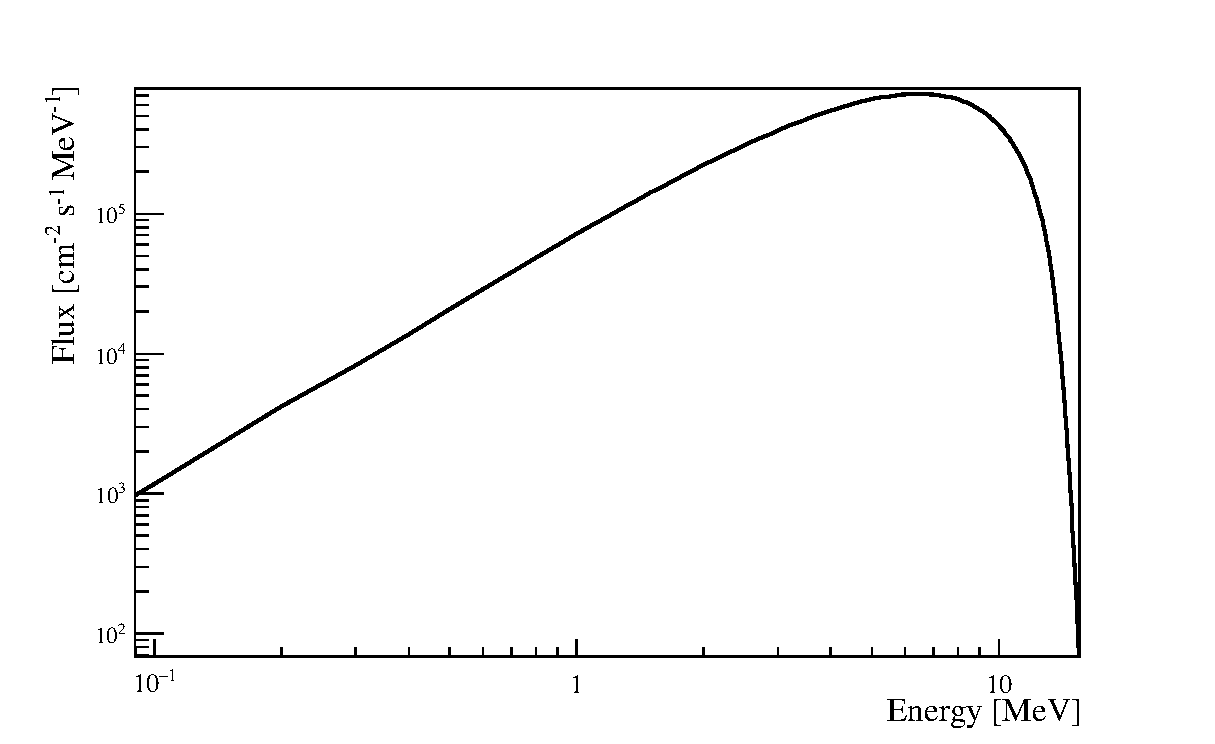
\includegraphics[width=0.75\textwidth]{b8_flux}
\caption[Expected $\ce{^{8}B}$ Flux]{The $\ce{^{8}B}$ neutrino flux
normalized to the solar reaction rate predicted by BS05-0P~\citep{bs_ssm}}
\label{fig:b8_flux}
\end{figure}

RAT, a Monte Carlo simulation of particle interactions in the detector is used
for predicting detector observables for solar neutrino and background events.
RAT is a Geant4-based~\citep{geant4} simulation that
contains a detector and DAQ simulation in addition to simulation of particle
interactions and photon propagation.

The first step in the Monte Carlo event simulation process is to generate
event vertex information, including the interaction location, and the neutrino
and recoil electron energy and direction.
The distribution for the $\ce{^{8}B}$ neutrino energy from Winters~\textit{et.\ al.}~\citep{winterspectrum}
was used, normalized to a nominal flux of
$\Phi_{\nu_{\mathrm{e}}} = 9.67\times10^{9}\mathrm{cm}^{-2}\mathrm{s}^{-1}$
and
$\Phi_{\nu_{\mathrm{\mu}}} = 5.46\times10^{10}\mathrm{cm}^{-2}\mathrm{s}^{-1}$.
These values are the full BS05OP~\cite{bs_ssm} $\ce{^{8}B}$ flux scaled by a factor
of $1700$ for the $\nu_{\mathrm{e}}$ and a factor of $9600$ for the $\nu_{\mathrm{\mu}}$.
The overall flux normalization is arbitrary in this analysis, but the enhanced rate
ensures that the statistical fluctuations observed in the MC datasets are
negligible compared to the detected dataset.

\begin{figure}[htbp]
  \centering
  \begin{subfigure}[b]{0.48\textwidth}
    \centering
  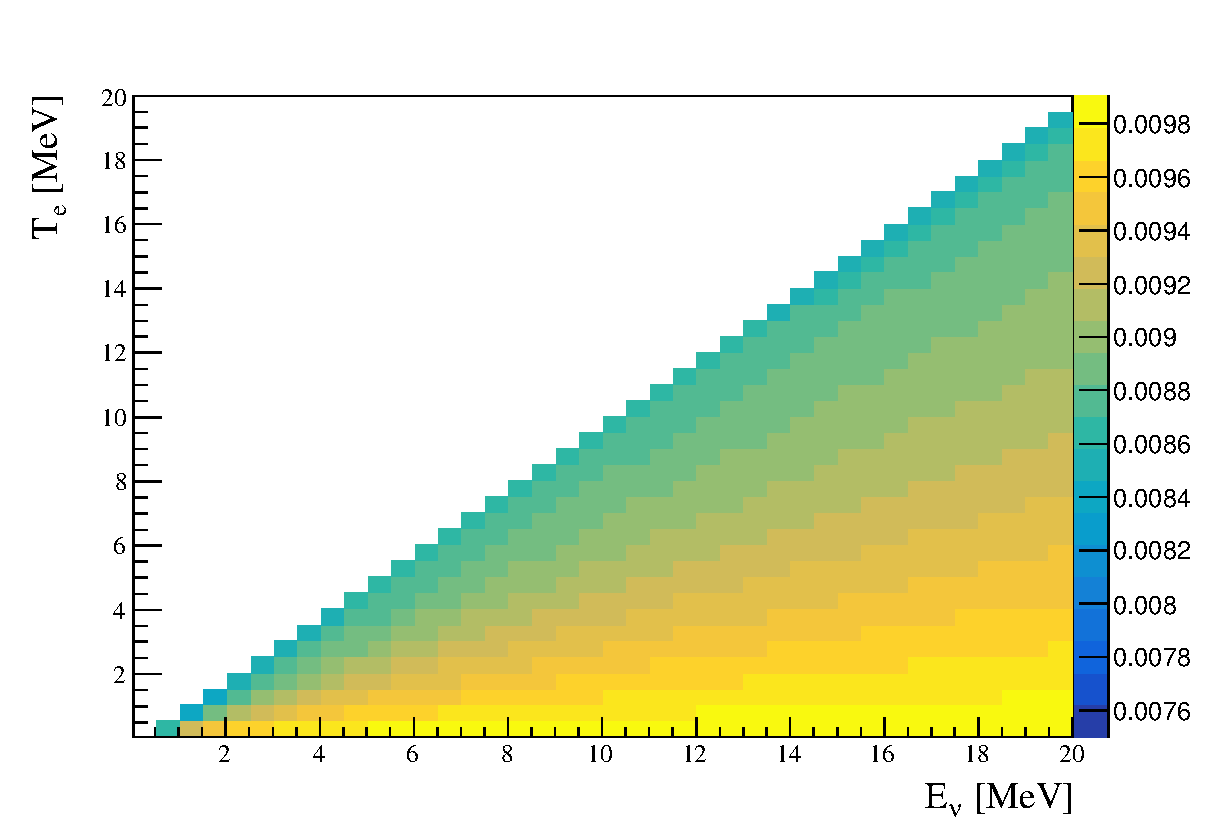
\includegraphics[width=\textwidth]{diff_xsec_nue}
    \caption[$\nu_{e}$ Differential Cross Section]{}
    \label{fig:diff_xsec_nue}
  \end{subfigure}
  \hfill
  \begin{subfigure}[b]{0.48\textwidth}
    \centering
  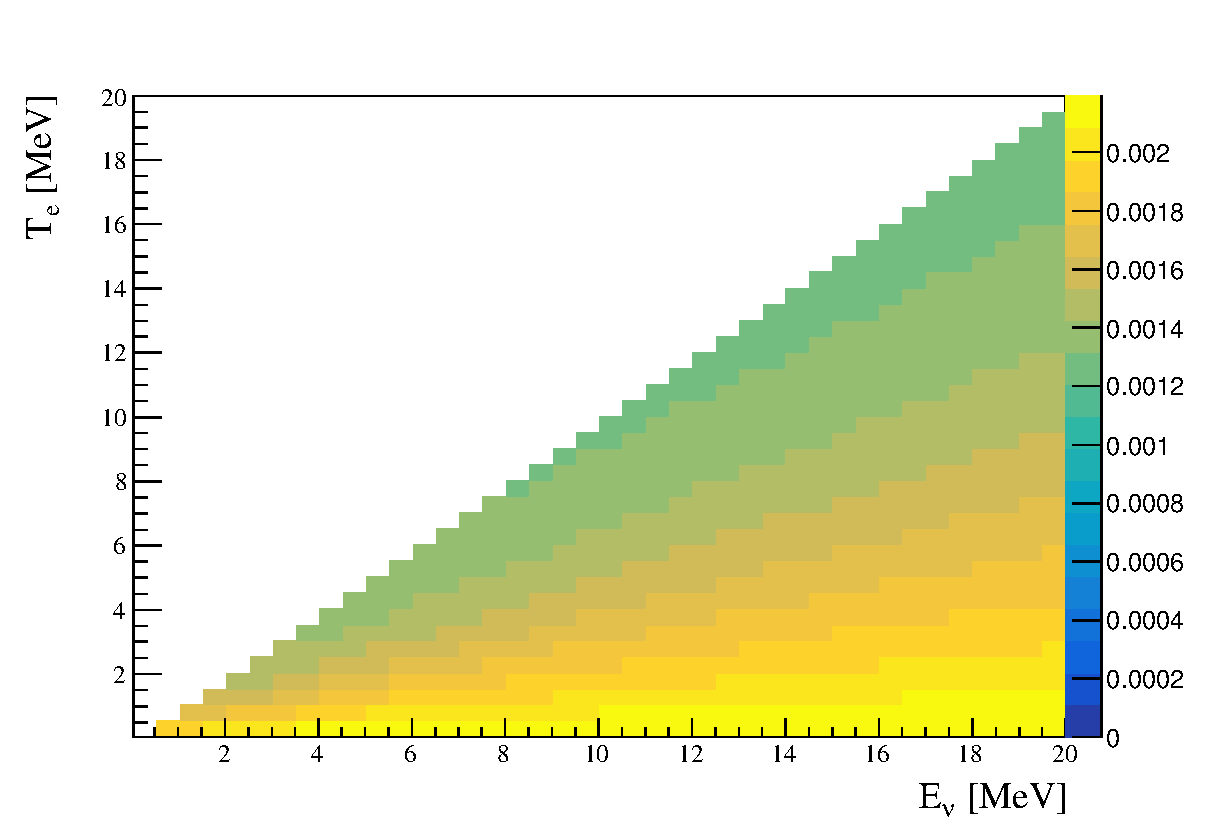
\includegraphics[width=\textwidth]{diff_xsec_numu}
    \caption[$\nu_{\mu}$ Differential Cross Section]{}
    \label{fig:diff_xsec_numu}
  \end{subfigure}
    \caption[ES Differential Cross Section]{The differential cross section for $\nu_{e}$ electron
    elastic scattering (a) and $\nu_{\mu\mathrm{,}\tau}$ (b) as used by
    RAT. Units for Z-axis is $10^{-42} \mathrm{cm}^{-2} \mathrm{MeV}^{-2}$.}
    \label{fig:diff_xsec}
\end{figure}

The rate of solar neutrino interactions for a given flux follows from the cross-section for
interaction. The only interaction relevant for this analysis is the
neutrino-electron elastic scattering interaction, the cross-section of which
is discussed in Sec.~\ref{sec:esxsec}.
The model used for event generation in RAT includes radiative corrections as
described in Bahcall~\textit{et. al}~\citep{escrosssec}.
The differential cross-section as a function of $E_{\nu}$ is shown in Fig.~\ref{fig:diff_xsec}.

\begin{figure}[htbp]
  \centering
  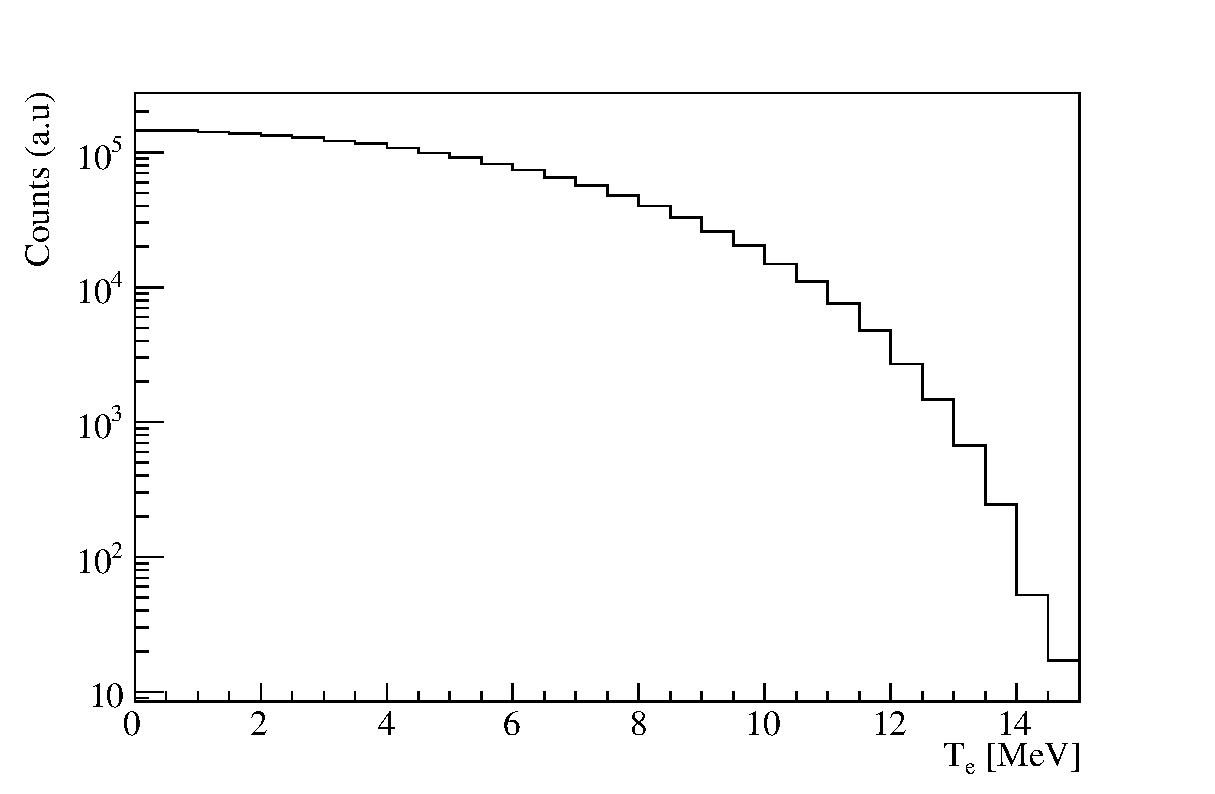
\includegraphics[width=\textwidth]{solar_nu_recoil_spectrum}
  \caption[Solar Recoil Electron Spectrum]{
      The distribution of electron recoil energies from $\ce{^{8}B}$ solar neutrino
      interactions, as simulated by RAT\@.}
    \label{fig:recoil_spectrum}
\end{figure}

Convolving the differential cross section with $\ce{^{8}B}$ neutrino flux
spectrum provides the expected event rate as a function of$T_{\mathrm{e}}$. 
RAT performs this convolution through Monte Carlo sampling of the neutrino
and cross-section PDFs.
The results of the MC sampling are show in Figure~\ref{fig:recoil_spectrum}.

Simulated recoil electrons are distributed uniformly throughout the SNO+ AV volume, with
the $\theta_{sun}$ given by,
\begin{equation}
  \cos\theta_{sun} = \sqrt{\dfrac{T_{\mathrm{e}}(m_{\mathrm{e}}+E_{\nu})^{2}}{2m_{e}E_{\nu}^{2} + E_{\nu}^{2}T_{\mathrm{e}}}}\text{.}
  \label{eqn:costheta_te}
\end{equation}
This equation assumes that the direction of the neutrino is directly from the center of sun.
Averaged over many events that is a safe assumption; the additional angular uncertainty
introduced by considering the radial neutrino production distribution is negligible.

Once the simulated position, direction, and energy of the recoil electron are determined  the
electron interactions and  photon production and propagation in the detector are simulated
by Geant4~\citep{geant4}.
The goal of this simulation is to transform the kinematics of the event to
a collection of PMT hits in the simulated detector.
In the simulation, once a photon interacts with a PMT photo-cathode, a check is performed
to simulate the detection efficiency for that photon, which includes the photo-cathode quantum efficiency and
PMT collection efficiency.
These efficiencies are determined from both \textit{ex-situ} PMT measurements
and~\textit{in-situ} calibration measurement.
The collection efficiencies are
taken to be uniform across the detector. %TODO Citation?
If the photon passes that check a PMT signal is created in the DAQ simulation.
Once all the photons in an event have been simulated and have either exited the detector,
been detected, or been absorbed, the DAQ simulation is run on the detected photon signals.

The goal of the DAQ simulation is to transform simulated PMT hits to detector observables,
\textit{e.g.} QHS, hit times, trigger information etc.
The DAQ simulation accomplishes this by replicating the trigger system of the real SNO+ detector.
It starts by creating waveforms for every simulated PMT signal, the size
of the PMT signal is drawn from the charge spectrum for each PMT as determined
by the PCA calibration.
Electronics noise is added to each simulated waveform, then each waveform is compared to a discriminator
threshold, the value for which is matched to detector settings.
For signals that pass the discriminator threshold a PMT hit is created
and N100, N20, ESUMH and ESUML trigger signals are produced.
The waveforms for the trigger signals are simulated with electronic noise and dropout, both
of which match detector measurements.
The trigger signals are then summed detector wide and compared to ``MTCA+'' thresholds.
If any of the threshold crossing signals are included in the simulated trigger mask
each hit's  QHS, QHL, QLX, and threshold crossing time, are calculated from the original PMT waveform.
The trigger waveforms are also digitized in a simulated 12-bit digitizer with sampling rate matched
to that of the CAEN v1720 digitizer.

\begin{figure}[htbp]
  \centering
  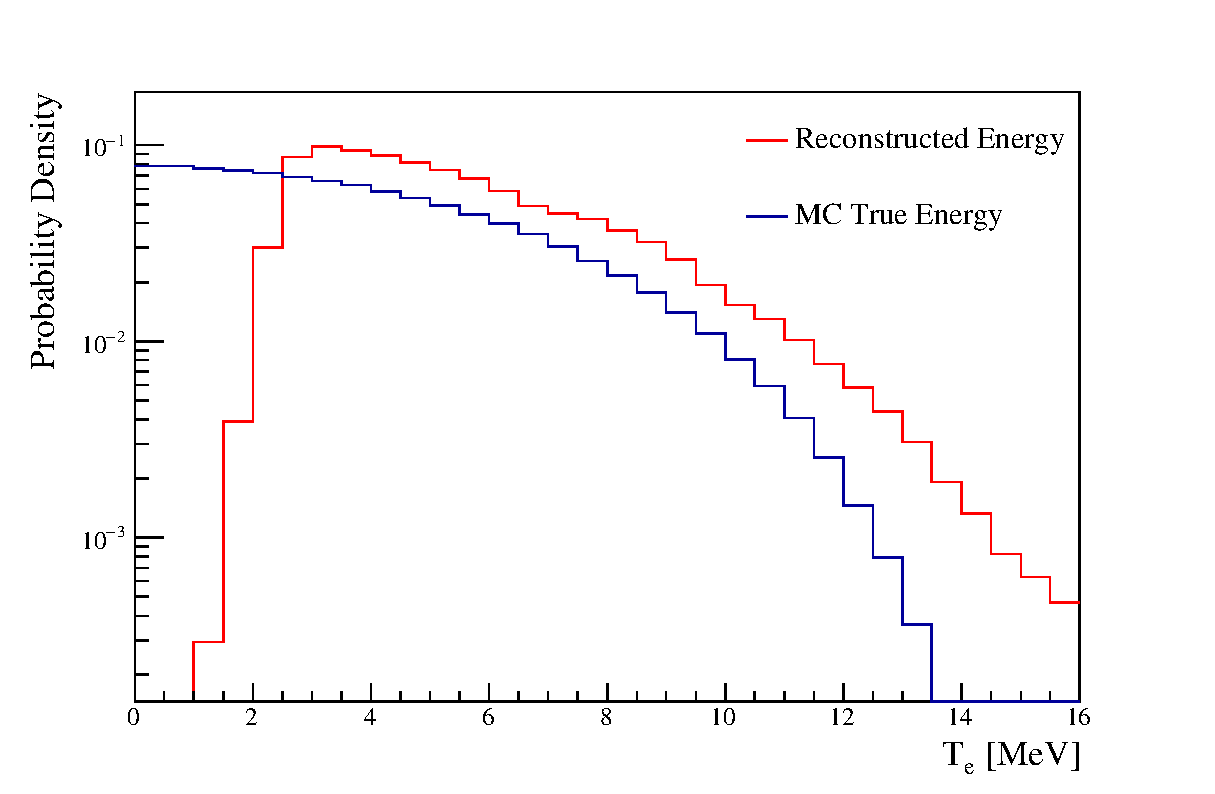
\includegraphics[width=0.7\textwidth]{energy_comparison}
  \caption[Reconstructed Energy Vs True Energy]{ The distributions of recoil
  electron truth energy (black) and reconstructed energy (red) for simulated
  $\ce{^{8}B}$ $\nu_{e}$ elastic-scatter events. Both histograms are normalized to $1.0$.} %TODO normalize them the number simulated instead
  \label{fig:energy_comparison}
\end{figure}

The result of the DAQ simulation is a dataset that can be used in exactly the same way the
detector data can be used.
Reconstruction is performed on the simulated detector observables 
 and the reconstructed quantities can be compared
to the corresponding MC truth values to assess expected detector performance.
The comparison between true energy and reconstructed energy is shown in
Fig.~\ref{fig:energy_comparison} for the simulated $\ce{^{8}B}$ $\nu_{e}$
dataset.
The probability of an event having a reconstructed energy below approximately 3\,MeV
is small because events with low energy will often not trigger the detector, or
fail to reconstruct at all.
Additionally to prevent the reconstruction process from being too computationally expensive
only 10\% of events with fewer than 15 PMT hits are reconstructed because
those events are generally not useful for analysis.

RAT is used to generate two MC datasets, a solar $\nu_{e}$ dataset
and a solar $\nu_{\mu}$ dataset.
No $\nu_{\tau}$ dataset is generated because the SNO+ detector has
no way to discriminate between $\nu_{\mu}$ and $\nu_{\tau}$ elastic scatters.
So the $\nu_{\mu}$ dataset can be considered to represent both the $\nu_{\mu}$
and the $\nu_{\tau}$ components of the solar neutrino flux.
The simulated solar neutrino datasets restrict interactions to the AV volume,
further datasets were generated that simulate interactions exclusively in the
volume between the AV and PSUP\@.
These external datasets contribute negligibly to the final dataset after all
analysis cuts are performed, and so they are in general not considered.

Also generated are a number of datasets for the expected backgrounds from
radioactive isotopes in various detector components.
These datasets are not directly used in this analysis, they were used however
for assessing the effectiveness of the analysis cuts that are used.

This analysis uses what is referred to as ``run-by-run'' simulation.
This means every detector data run used in the analysis has a simulated run that uses
the detector and electronic calibration settings from the run as input to the DAQ simulation, and simulates
a length of time and time of day equal to the detector run.
The purpose of this is to remove the possibility that changes in detector settings
or circumstances will bias any result.
This method is not perfect, there exists features of the real detector
that are not simulated.
For example, it's known that human activity around the DAQ electronics can generate
noise on the front end, this sort of noise source can be difficult to directly observe
in the detector data and cannot be simulated.
For this reason detector runs that have difficult to simulate conditions
are typically not included in the analysis, this is discussed further
in Sec.~\ref{sec:data_selection}.

\section{Survival Probability Simulation}
\label{sec:survival_prob}
\begin{figure}[htbp]
\centering
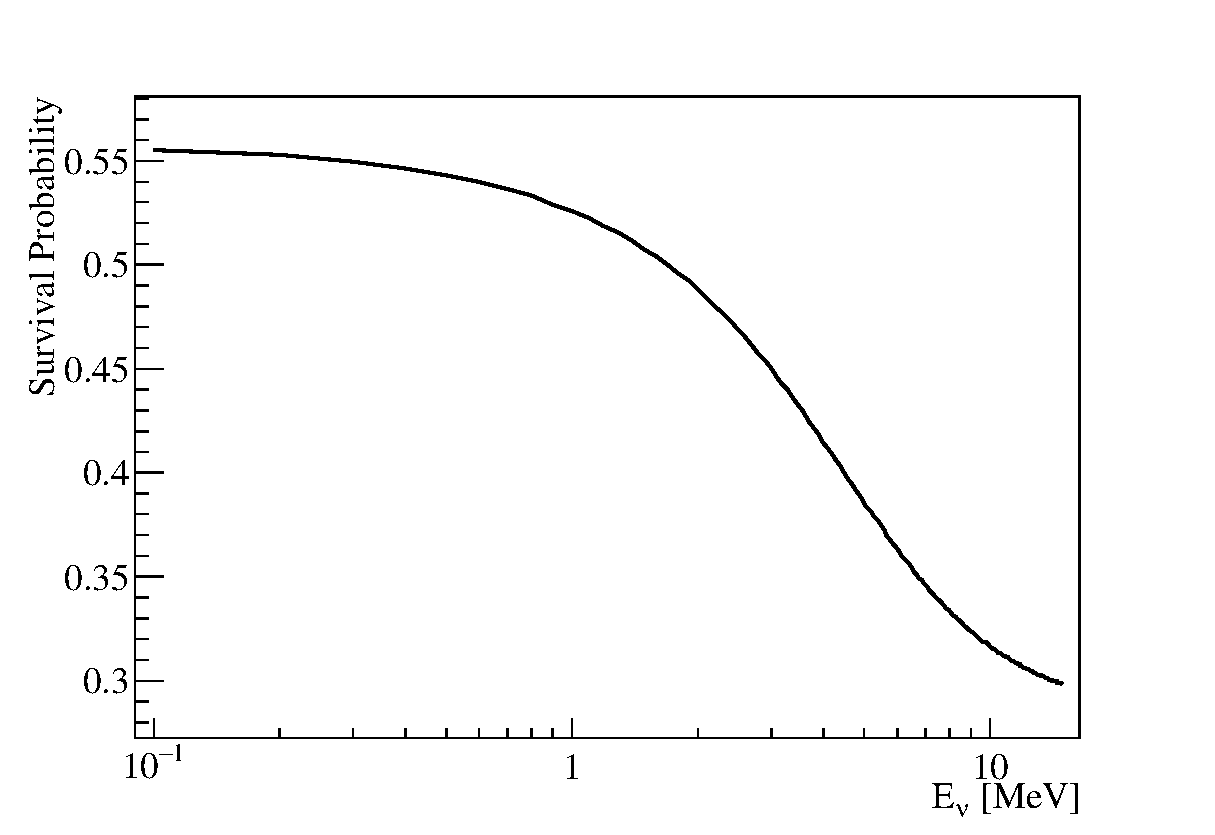
\includegraphics[width=0.75\textwidth]{pee_example}
\caption[$\ce{^{8}B}$ Solar Neutrino Survival Probability]{
Survival probability for $\ce{^{8}B}$ solar neutrinos for mixing parameters
given in table 1 of Capozzi~\textit{et.\ al.}~\citep{pdg_globalfit}.
}
\label{fig:example_survival_prob}
\end{figure}

The neutrino survival probability is simulated outside of RAT\@.
The MC $\nu_{\mathrm{e}}$ and $\nu_{\mathrm{\mu}}$ datasets are combined
as one of the last stages of this analysis to ensure that MC data
does not need to be regenerated for any change in the simulated survival probability.

The survival probability is calculated using a three-flavor adiabatic approximation.
The implementation used is the Physics interpretation Sun-Earth Large Mixing Angle Adiabatic Approximation
(PSelmaa) used in SNO~\citep{nuno_thesis, sno_combined}.
The survival probability calculation use the GS98~\citep{gs98} solar abundances
and the BS05OP radial production distributions and solar density profile~\citep{bs_ssm}.
Figure~\ref{fig:example_survival_prob} shows an example survival probability, using the best fit mixing parameters
from a global fit to neutrino oscillation data~\citep{pdg_globalfit}.
The uncertainties on those values are also considered as will be discussed in
Sec~\ref{sec:systematics}.

\chapter{Reconstruction}
\label{sec:reconstruction}
A series of reconstruction algorithms are run over all events that pass data cleaning.
These algorithms estimate the position, time, direction, and energy of the event.
All events are reconstructed under the hypothesis that the PMT hits are from Cherenkov radiation
produced by a single electron.
Additionally, the reconstruction algorithms use only the hits in a prompt time window to ensure only light
that travelled directly from the event origin is used,
though each algorithm defines differently window is used.
Only hits that are from well calibrated, online PMTs and detector channels are used.
%The reconstruction algorithms used in this analysis are all algorithms that were developed for SNO\@.
%Since having a light-water vs heavy-water target has small and easily accounted for effects on the emission of Cherenkov radiation inside the AV, these algorithms perform effectively for the SNO+ water phase as they did for SNO\@.
The same reconstruction algorithms are used on both simulated and detected events.

The direction ($\vec{d}$), time ($t_{0}$), and position ($\vec{p}$) are determined by performing a likelihood
fit to the time and position of PMT hits.
Only hits within a $100$\,ns window centered around the mode of the raw hit time
distribution are used.
The algorithm evaluates the likelihood of a hypothesized event position and time by
calculating the time residual for each hit PMT,
\begin{equation}
\label{eqn:tres}
t_{res} = t_{PMT} - t_{transit} - t_{0}\text{.}
\end{equation}
The transit time is calculated by considering the distance the photon would
traverse in inner volume water, the external water, and inside the AV acrylic, as
it travels from the hypothesized position to the PMT, accounting for refractions
at boundaries.
From those distances the transit time is simply calculated as
\begin{equation}
t_{transit} = \frac{d_{\mathrm{AV}}}{v_{\mathrm{AV}}} + \frac{(d_{\mathrm{inner}} + d_{\mathrm{external}})}{v_{\mathrm{water}}}\text{,}
\end{equation}
the group-velocity for 400\,nm light is used as the velocity.

\begin{figure}[htbp]
\centering
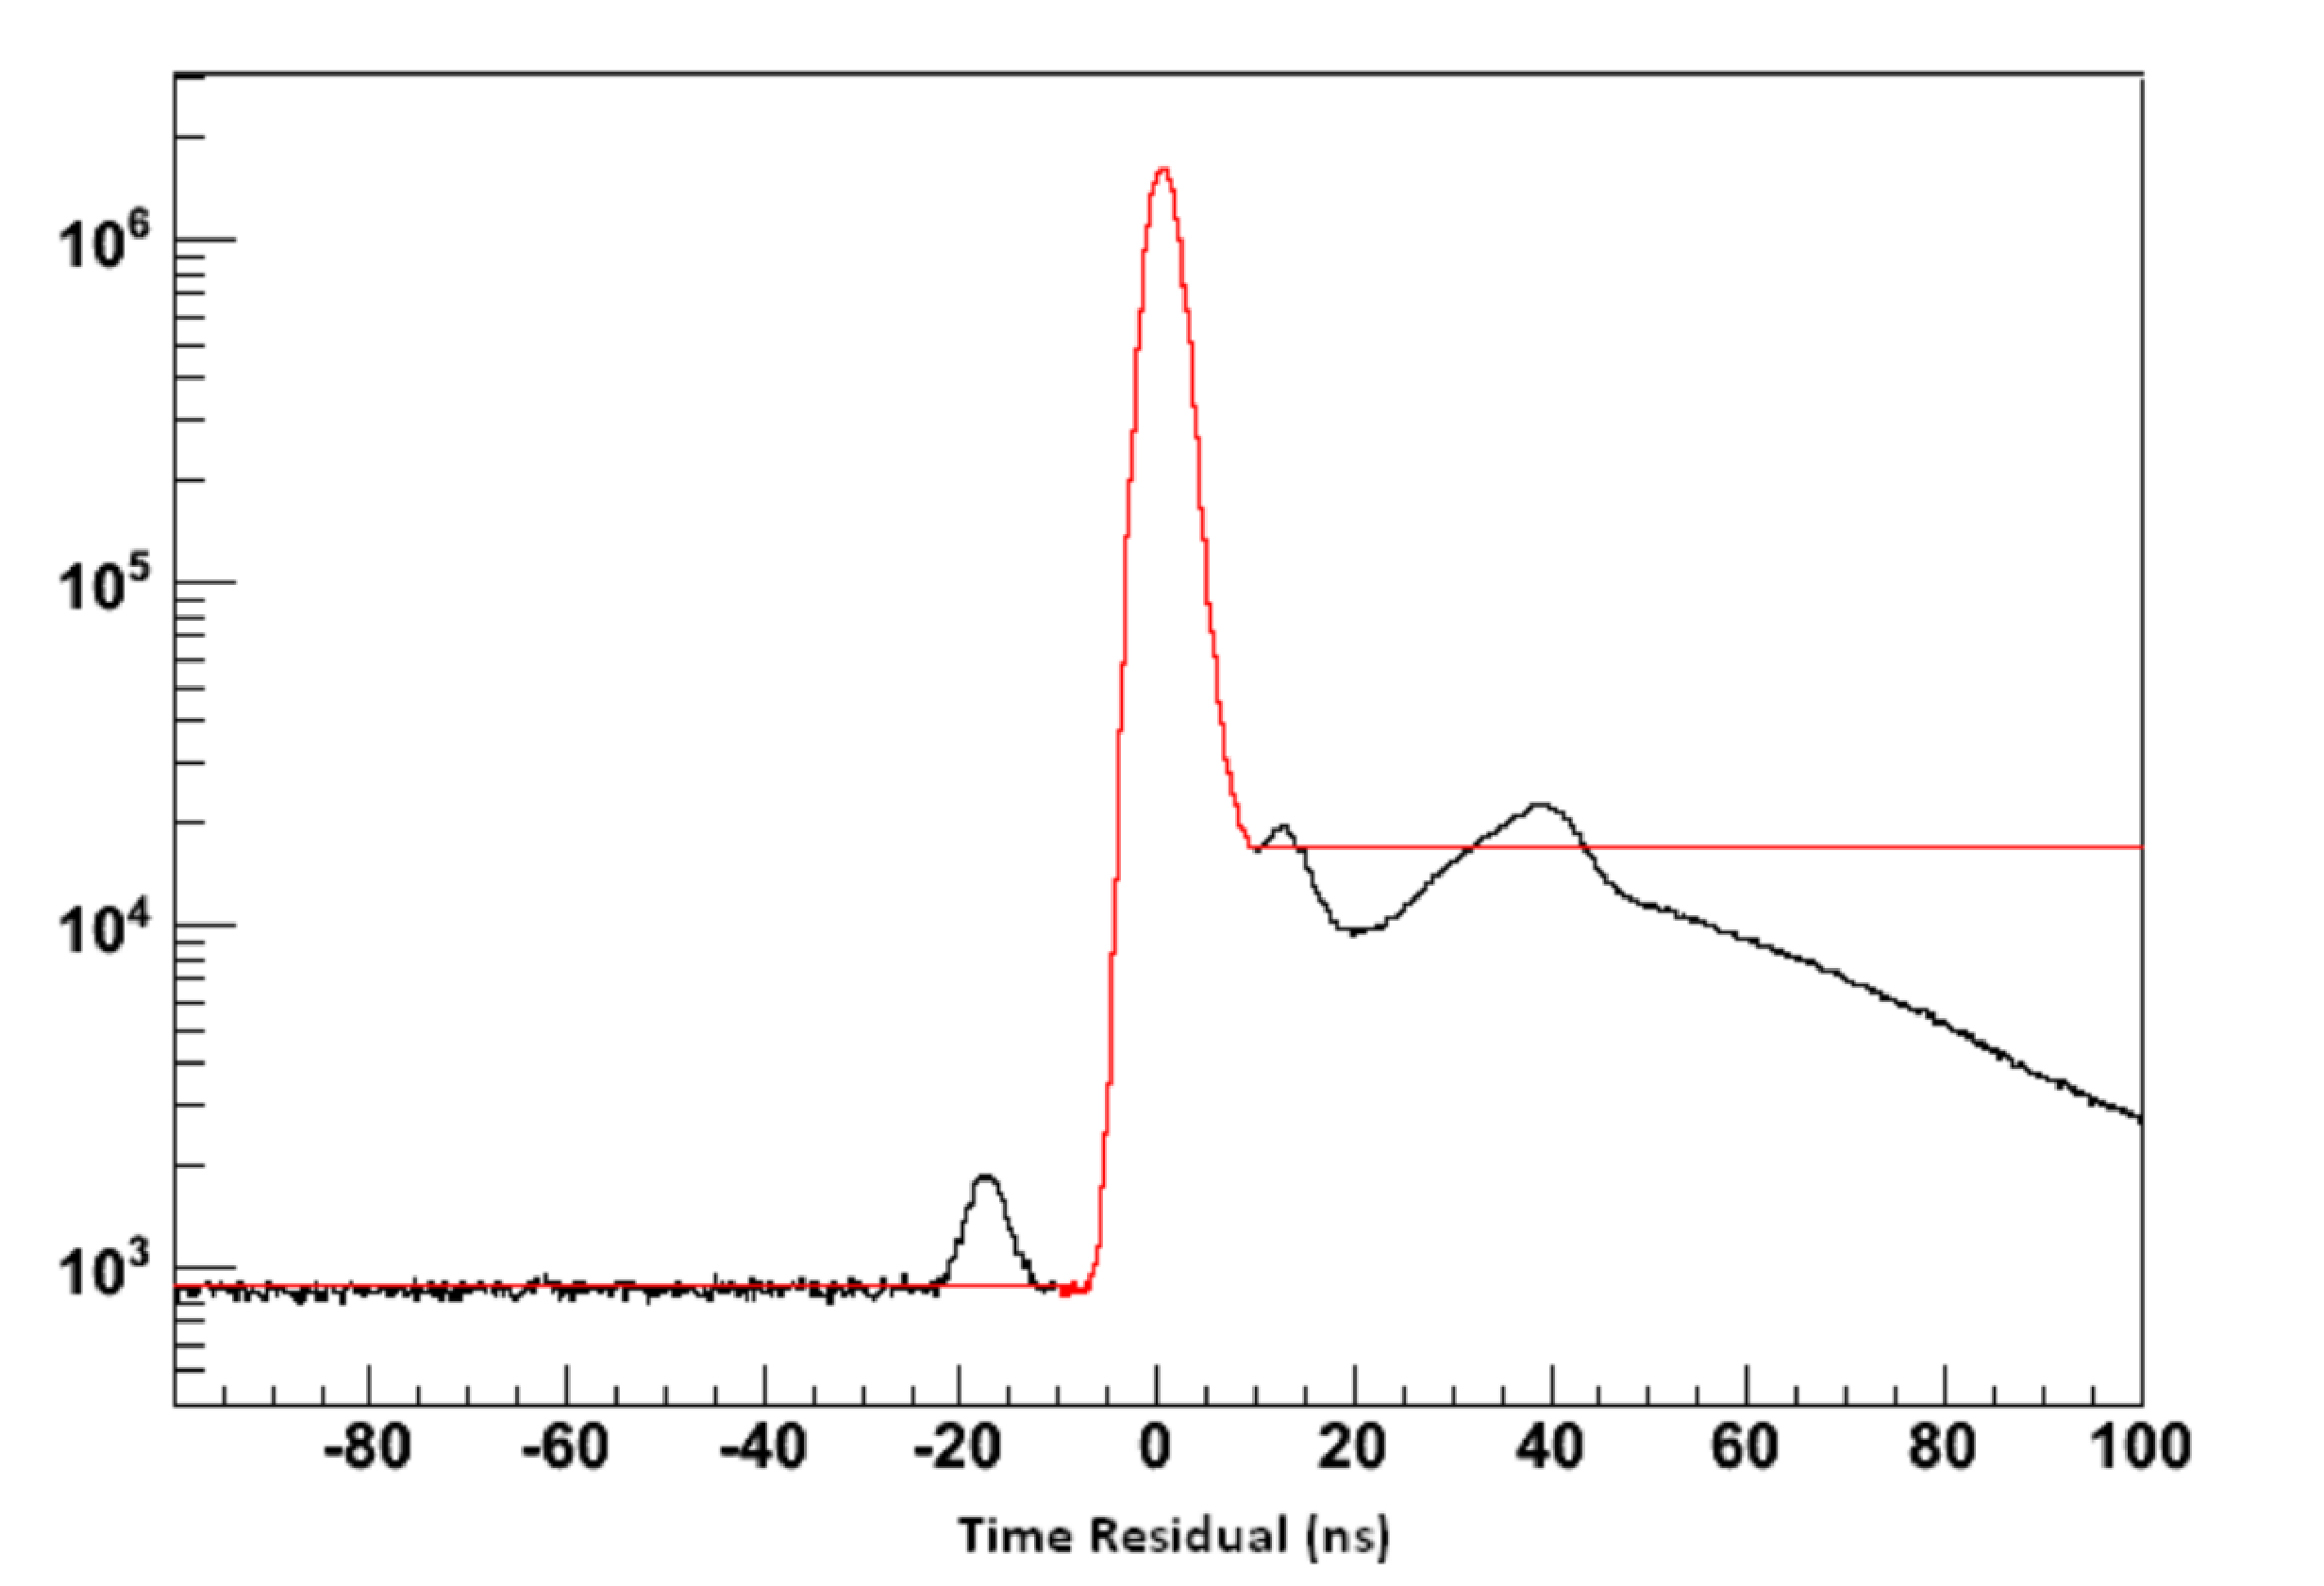
\includegraphics[width=0.78\textwidth]{tres_dist}
\caption[Simulated Distribution of $t_{\mathrm{res}}$]{
(black) Distribution of time residuals for simulated 6\,MeV electrons. (red) Simplified
timing distribution used for reconstruction. Figure from~\citep{richie_thesis}.}
\label{fig:tres_dist}
\end{figure}

The PDF for $t_{\mathrm{res}}$, $P(t_{\mathrm{res}})$, is determined from prior simulation,
Fig.~\ref{fig:tres_dist} shows this PDF compared to a full timing simulation.
The position and time that minimize the quantity
\begin{equation}
\sum_{i=0}^{N_{PMT}} P(t_{res}) % TODO need to refactor this to include the index i
\end{equation}
is used as the event position and time.

The direction is determined by evaluating $\theta_{\mathrm{PMT}}$ for each hit where
$\theta_{\mathrm{PMT}}$ is defined by,
\begin{equation}
    \cos\theta_{\mathrm{PMT}} = \vec{d}\cdot\left(\vec{p}_{PMT} - \vec{p}\right)\text{.}
\end{equation}
The likelihood, $P(\theta_{\mathrm{PMT}})$, is determined from a prior simulation of
6\,MeV electrons at the center of the detector, Fig~\ref{fig:rat_angle_pdf} shows
this PDF\@. %That PDF is modified by a correction to account for the fact that PMTs nearer to the event vertex are more likely to be hit.
The direction that minimizes
\begin{equation}
\sum_{i=0}^{N_{PMT}} P(\theta_{\mathrm{PMT}})
\end{equation}
is used as the reconstructed event direction.

\begin{figure}[htbp]
\centering
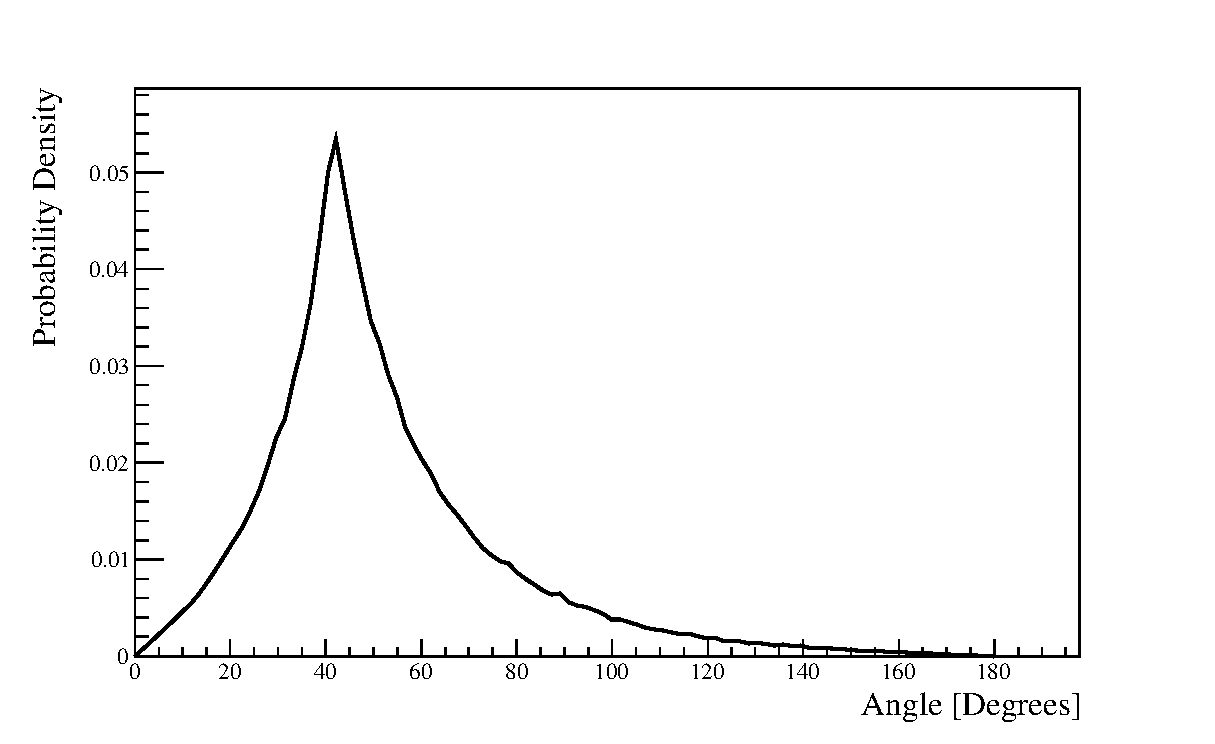
\includegraphics[width=0.78\textwidth]{rat_angle_pdf}
\caption[RAT PDF for Direction Fit]{The PDF used by RAT when evaluating the
likelihood of a hypothesized direction.  The peak at approximately $40^{\circ}$
corresponds to the Cherenkov cone opening angle.}
\label{fig:rat_angle_pdf}
\end{figure}

The kinetic energy of the event is determined after
the event position, time and direction are determined.
The position and time are used to determine the number of PMT
hits that occurred in a prompt 18\,ns window.
Then the number of photons that would most likely produce
that number of PMT hits is estimated using a combination of
analytic calculation and PDFs from prior simulation.
A look up table is used to estimate the most likely electron
kinetic energy that would produce the determined number of photons.
This method of energy reconstruction is called ``EnergyRSP'', which stands
simply for Energy Response.

\begin{figure}[htbp]
\centering
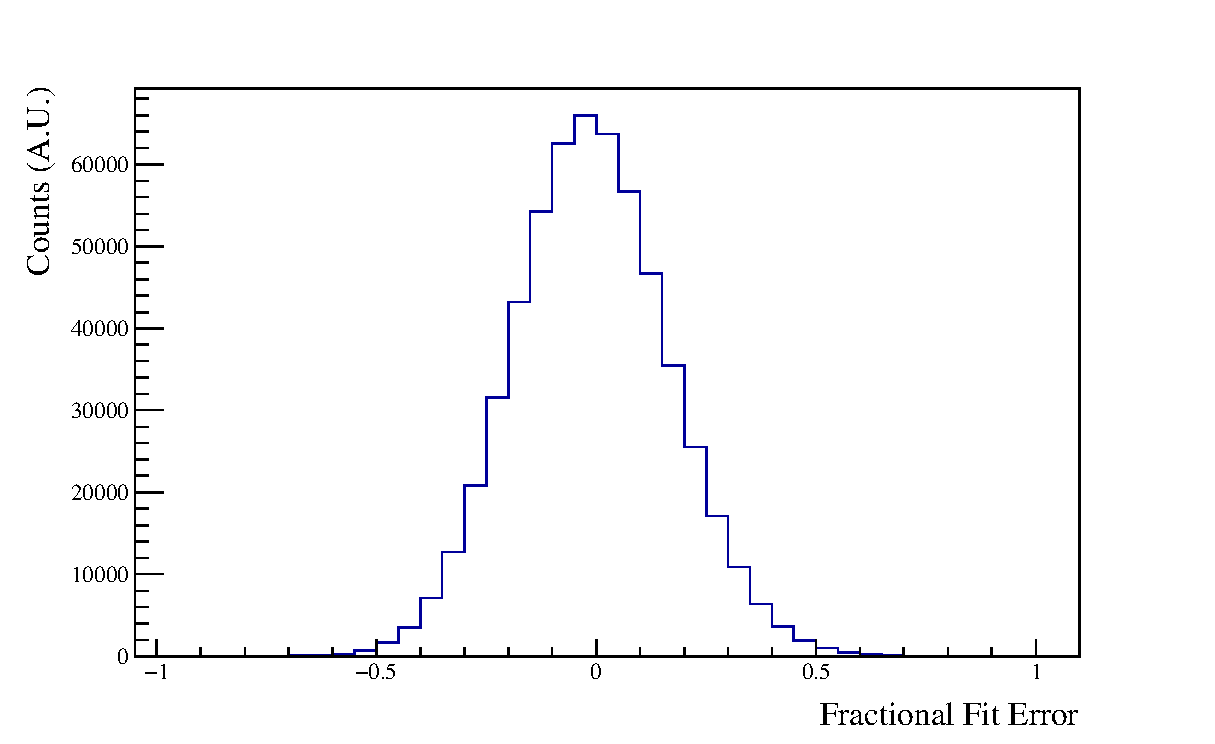
\includegraphics[width=0.78\textwidth]{fit_residual_nofit}
\caption[EnergyRSP Fit Residuals]{Fractional error of fitted energy   for solar $\nu_{\mathrm{e}}$ events
with simulated energy above 5\,MeV.
}
\label{fig:mc_fit_residuals}
\end{figure}
The uncertainty in the energy fit is dominated by the uncertainty
introduced by the photon-statistics associated with Cherenkov radiation.
For electrons the number of detected photons per MeV kinetic energy is approximately 7.
Meaning a 5\,MeV electron event will on average produce 35 PMT hits with
one-sigma statistical fluctuations of roughly $\sqrt{35} \approx 5.9$, or about 17\%.
Figure~\ref{fig:mc_fit_residuals} shows the residuals for fit results on MC simulated solar $\nu_{e}$ events.

%An error was found in the calculation of the number of Cherenkov photons expected for an electron of a given energy.

\section{Calibration}
\label{sec:calib}
The accuracy of simulated events is evaluated with data taken while a
radioactive source was deployed within the detector volume.
For this analysis an $\ce{^{16}N}$ source was used.
The SNO+ $\ce{^{16}N}$ source was developed for SNO, as
their primary energy calibration source~\citep{sno_n16}.
The methods and results of SNO+'s $\ce{^{16}N}$ calibration are summarized here but
are described in greater detail by~\citep{snop_water_unidoc}.

\begin{figure}[htbp]
\centering
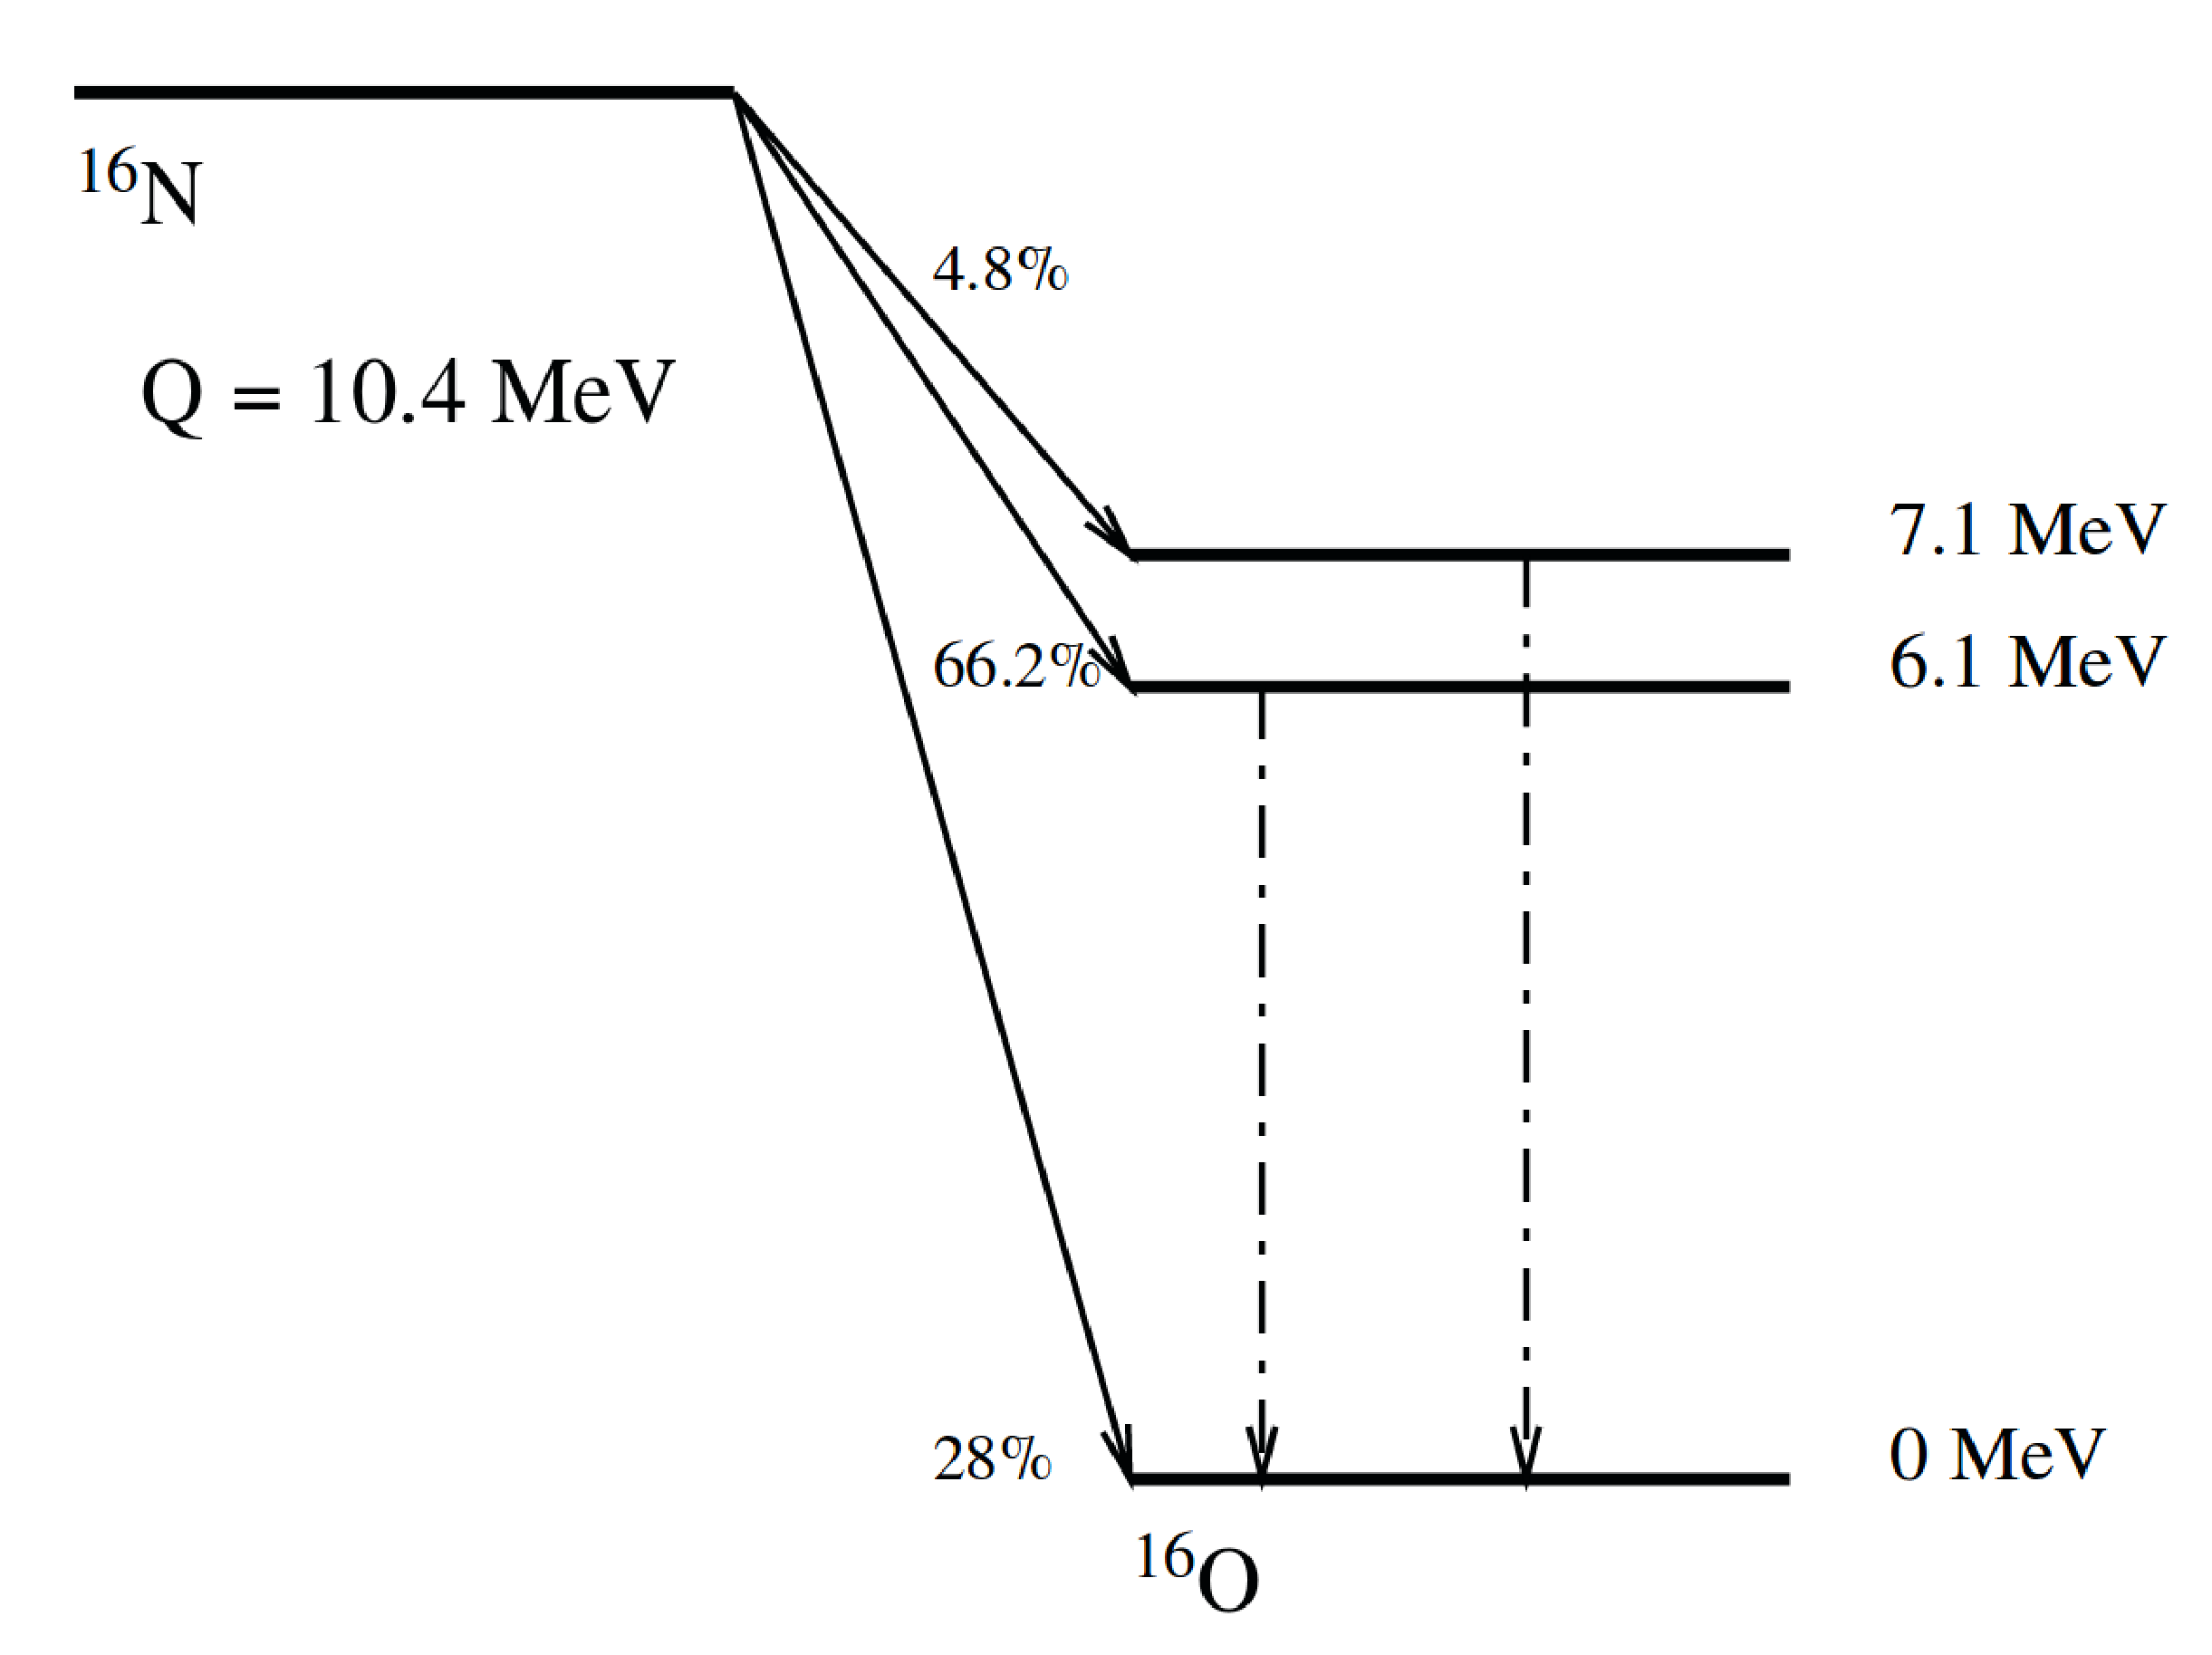
\includegraphics[width=0.58\textwidth]{n16_branching_ratios}
\caption[Major $\ce{^{16}N}$ Branching Ratios]{The most significant branching ratios for $\ce{^{16}N}$ decaying
to an excited state of $\ce{^{16}O}$. Figure from~\cite{sno_n16}.}
\label{fig:n16_br}
\end{figure}
The $\ce{^{16}N}$ source was developed by SNO, it uses a commercial
deuterium and tritium generator (DT-generator) to produce gaseous $\ce{^{16}N}$.
The gas is pumped into the deployed source where it can undergo $\beta$-decay
to an excited state of $\ce{^{16}O}$, the $\ce{^{16}O}$ will then de-excite
and typically emit a $6.1$\,MeV gamma particle. Higher or lower energy gammas are emitted
at a lower rate, the branching ratios for the de-excitation gammas are shown in
Fig~\ref{fig:n16_br}.

A small block of plastic scintillator, observed by a PMT, is embedded within the
source cannister. The PMT detects the $\beta$ from the initial
$\ce{^{16}N} \rightarrow \ce{^{16}O^{*}}$ decay. That PMT signal is used as a
tag in the detector DAQ to identify events from the deployed source.

The source position within the AV was varied in a 3-dimensional
scan.
A 1-dimensional scan was done along the z-axis between the AV and PSUP\@.
Scanning many positions allowed for a position dependent evaluation of
systematics and a position dependent correction to the reconstructed energy.

\subsection{Energy Calibration}
The detector resolution $\sigma_{E}$ and relative energy scale $\delta_{E}$ are determined
from the $\ce{^{16}N}$ energy spectrum.
The energy spectrum is modeled by $P(T_\mathrm{e})$, the energy spectrum in
electron equivalent kinetic energy, and is given by $P_{\mathrm{source}}(T_{\mathrm{e}})$
convolved with a normalized Gaussian distribution,
\begin{equation}
    P(T_\mathrm{e}) = N \int P_\mathrm{source}(T^{\prime}_{e})\frac{1}{\sqrt{2\pi}\sigma_{E}}e^-{\frac{\left((1+\delta_E)T_\mathrm{e}-T^{\prime}_{e}\right)^{2}}{2\sigma^{2}_{E}}}dT^{\prime}_{e}\text{.}%-\Delta E
\label{eq:convolution}
\end{equation}
$P_\mathrm{source}(T_{\mathrm{e}})$ represents the distribution of deposited energy in
the detector from the $\ce{^{16}N}$ source, in electron equivalent energy.
Since the $\ce{^{16}N}$ emits gammas into the detector the mapping between
gamma energy and electron equivalent energy is done by finding the electron
energy that can produce the same number of Cherenkov photons
as each gamma; this is not a one-to-one mapping because the same electron or gamma
energy will not always produce the same number of photons.
The mapping is determined from simulation and is shown in
Fig.~\ref{fig:cherenkov_energy_map}.
The gamma to electron energy mapping is then applied to the simulated $\ce{^{16}N}$
gamma energy spectrum to determine $P_\mathrm{source}(T_{\mathrm{e}})$.

\begin{figure}[htbp]
\centering
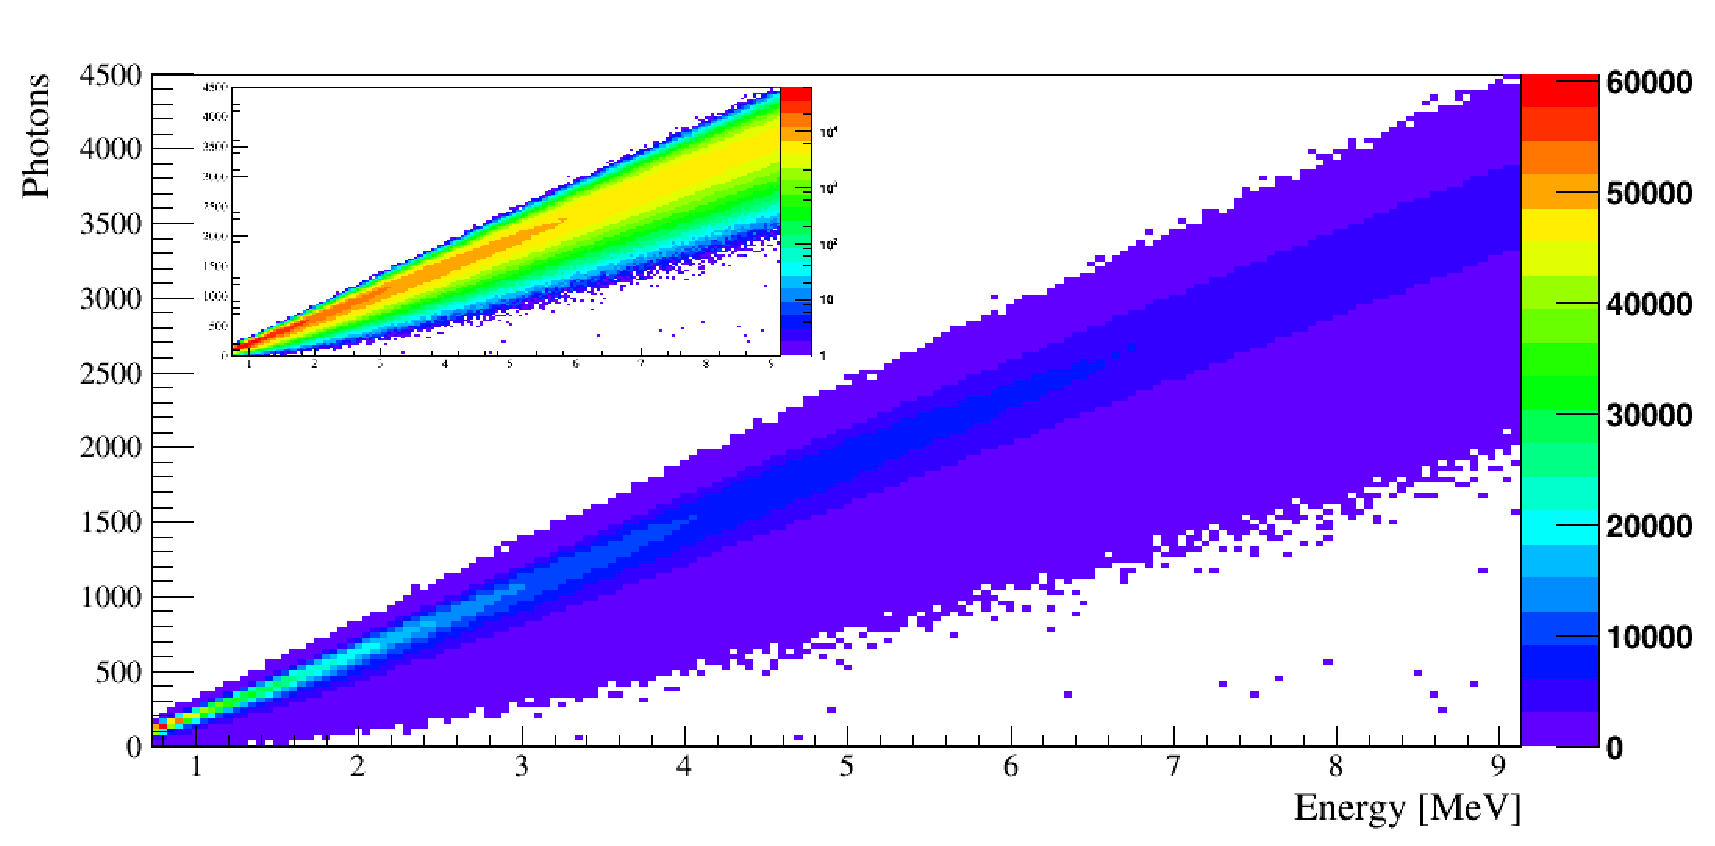
\includegraphics[width=0.78\textwidth]{cherenkov_nhit_energy_map.eps}
\caption[Electron Cherenkov Photon Product PDF]{ The map between electron
energy and expected Cherenkov photons production.  Used for the energy
calibration to map between gamma energy and equivalent electron energy.  This is
the same PDF used by EnergyRSP to estimate energy from the observed PMT hits.}
\label{fig:cherenkov_energy_map}
\end{figure}

\begin{figure}[htbp]
\centering
\begin{subfigure}{0.48\textwidth}
\centering
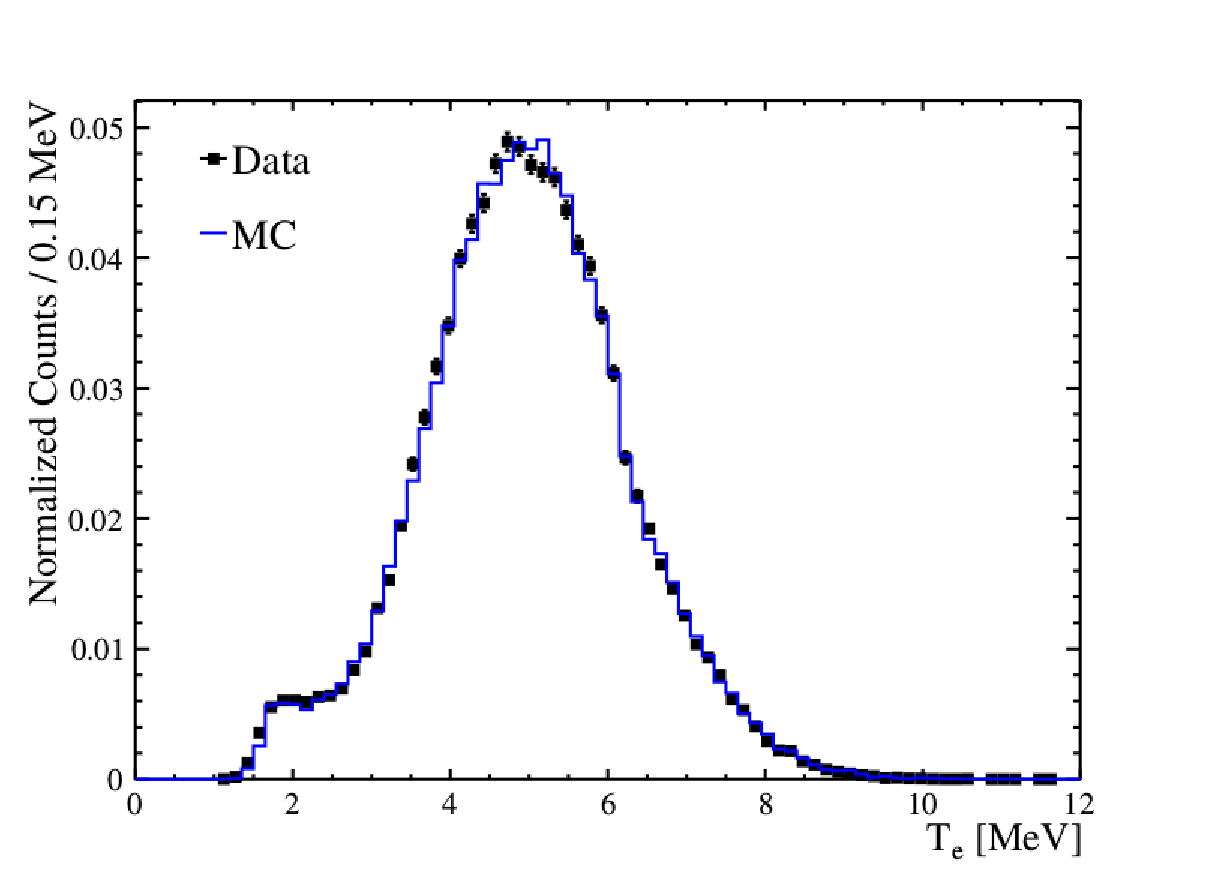
\includegraphics[width=\textwidth]{energy_data_vs_mc}
\caption[]{}
\end{subfigure}
\hfill
\begin{subfigure}{0.48\textwidth}
\centering
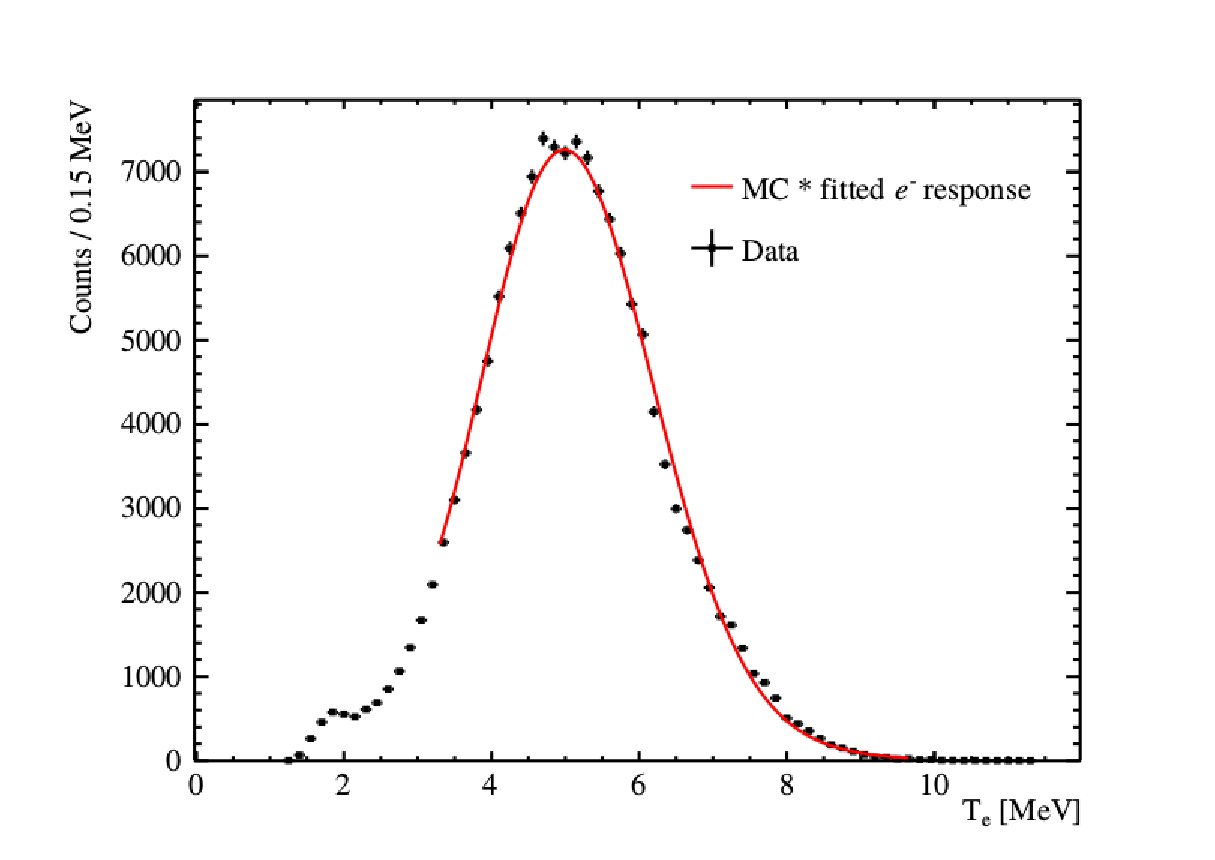
\includegraphics[width=\textwidth]{N16energyFit}
\caption[]{}
\end{subfigure}
\caption[$\ce{^{16}N}$ Energy Comparisons]{ (a) The comparison between
reconstructed energy for $\ce{^{16}N}$ data and monte-carlo.  (b) Fit of
Eqn.~\eqref{eq:convolution} to distribution of reconstructed energies for
detected central $\ce{^{16}N}$ events.}
\label{fig:n16_energy}
\end{figure}
The values for $\sigma_{E}$ and $\delta_{E}$ are extracted from~\eqref{eq:convolution}
by performing a fit to the reconstructed $\ce{^{16}N}$ energy spectrum.
The fit is done to both simulated $\ce{^{16}N}$ data and to detector data,
each determining their own values for $\sigma_{E}$ and $\delta_{E}$.
As is show in Fig~\ref{fig:n16_energy}, this fit is only performed
over the energy range $3.25$ to $9.6$\,MeV, at energies outside this range
difficult to model source-container effects dominate the energy spectrum.
It's worth noting that $\sigma_{E}$ represents only the resolution provided by detector
effects, resolution from effects such as photon statistics are accounted
for in $P_\mathrm{source}(T_{\mathrm{e}})$.

Values for $\sigma_{E}$ and $\delta_{E}$ are extracted for data taken, or simulated, with
the $\ce{^{16}N}$ source at many position, allowing for a position dependent
determination of the energy scale and resolution.
Fitting to both simulated and to detected data allows for a correction to
be created that can make the two datasets match better, however the data
used to create the correction cannot then be used to determine systematics.
So the $\ce{^{16}N}$ data was split into two datasets, one for determining
what correction should be applied to simulation, the other for extracting systematics
after the correction is applied.

The data for the correction is further divided into position bins in $z$ and
$\rho$, where $\rho = \sqrt{x^{2} + y^{2}}$. The choice of binning is motivated
by the symmetry of the detector, the detector is very symmetric for an interchange
of $x$ and $y$ or $x,y \rightarrow -x,-y$.
There exists, however, significant asymmetries along the $z$ axis
from the detector neck and from the rope-net along the top of the AV\@.
The data is divided into 4-bins along the $\rho$ direction each $200$\,cm long
and bins of $57$\,cm height along the $z$ axis. The number of bins along the
z-axis varies for each slice in $\rho$ because data was primarily taken within
the AV.\@
Figure~\ref{fig:n16_uniformity} shows position dependence of the fits for
$\delta_{E}$ and $\sigma_{E}$ in each bin for both simulated and detected
events.

\begin{figure}[htbp]
\centering
\begin{subfigure}{0.49\textwidth}
\centering
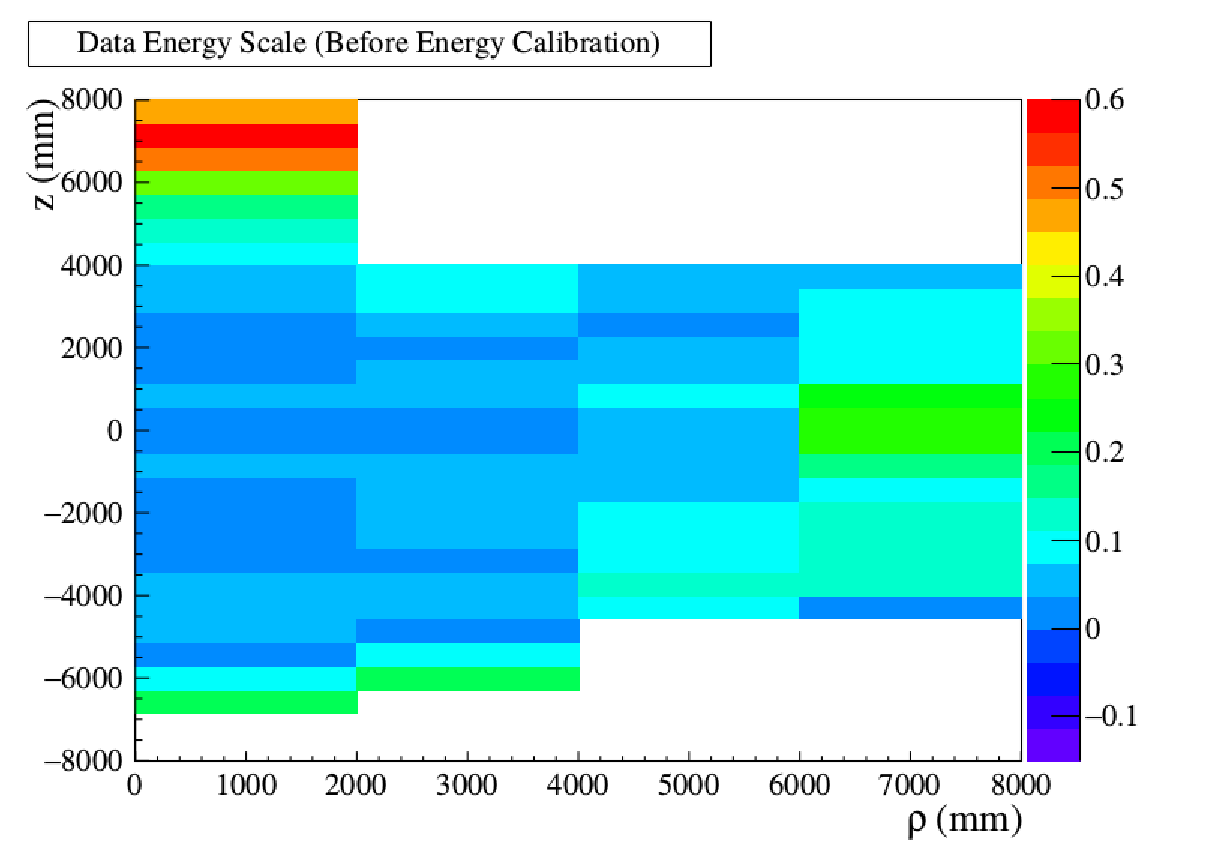
\includegraphics[width=\textwidth]{data_scale_uniformity}
\caption[]{}
\end{subfigure}
\hfill
\begin{subfigure}{0.49\textwidth}
\centering
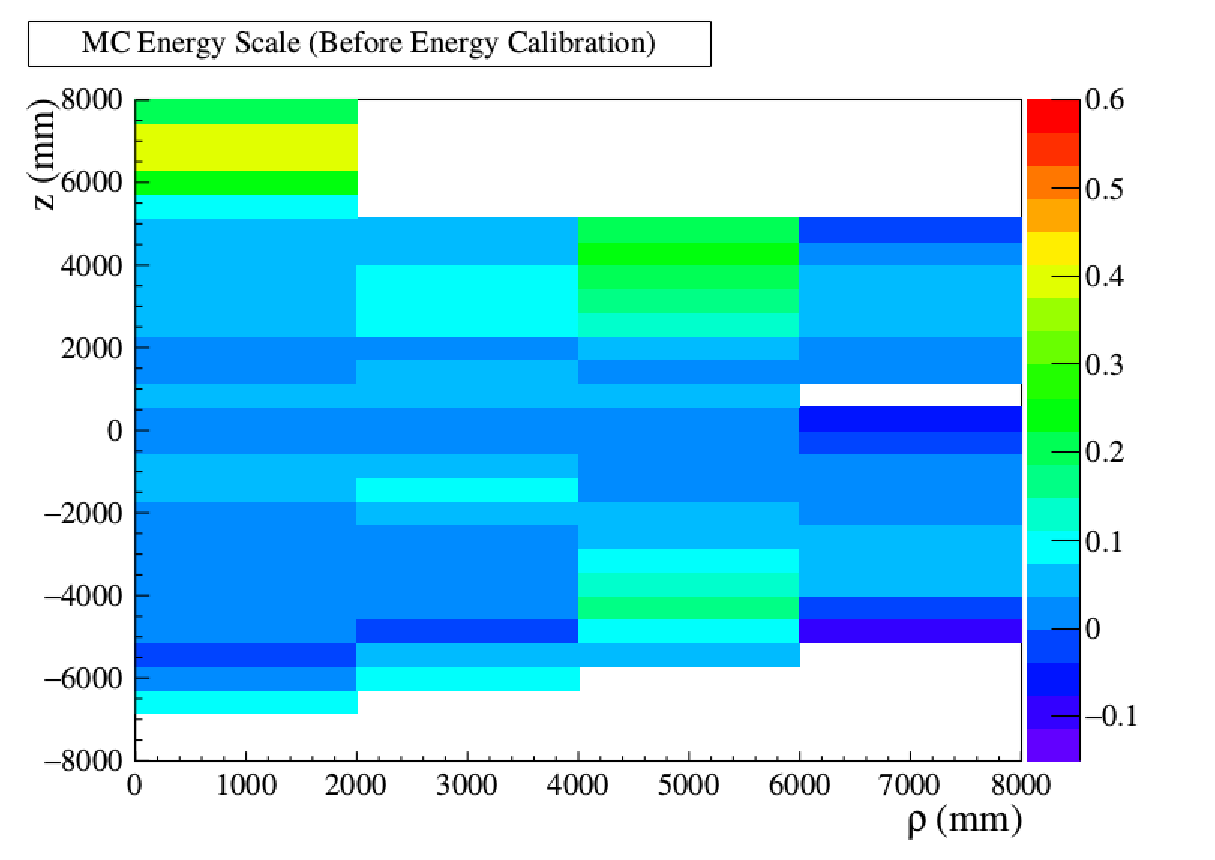
\includegraphics[width=\textwidth]{mc_scale_uniformity}
\caption[]{}
\end{subfigure}

\begin{subfigure}{0.49\textwidth}
\centering
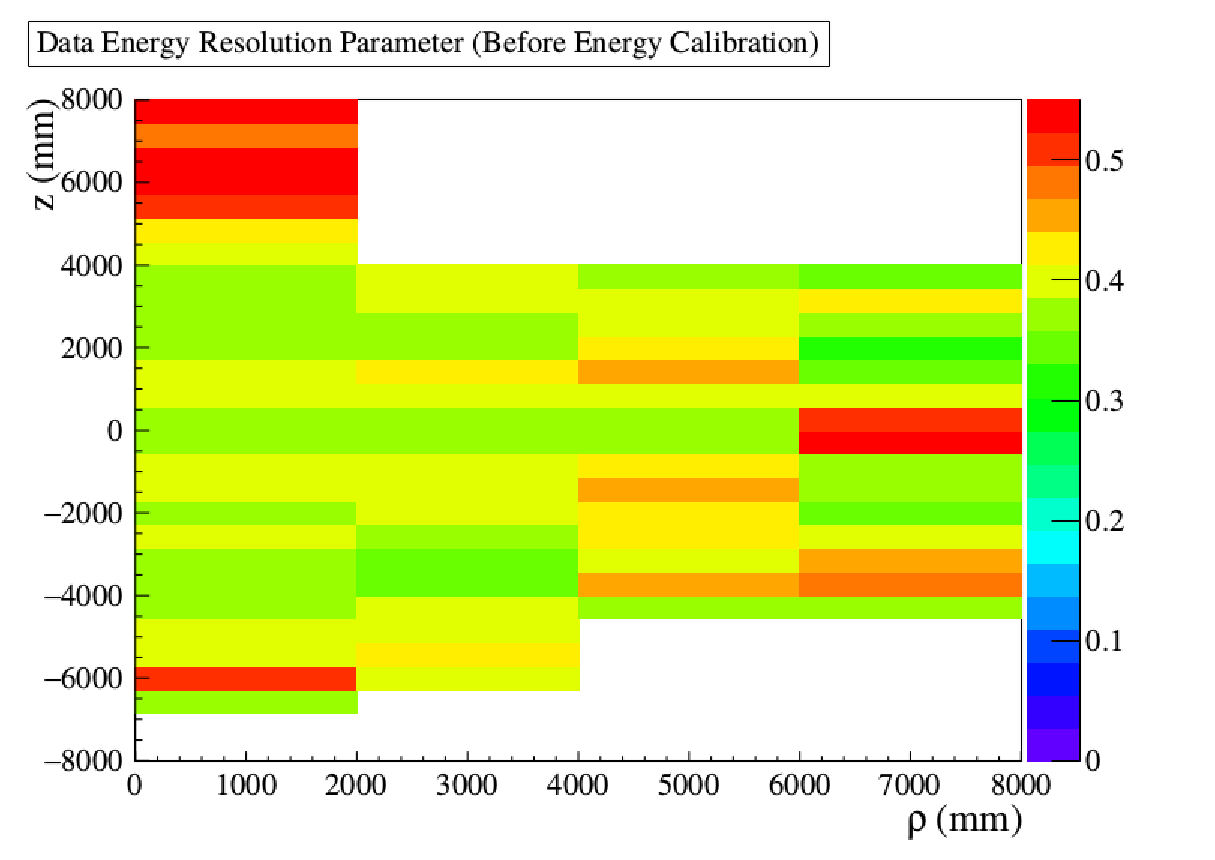
\includegraphics[width=\textwidth]{data_sig_uniformity}
\caption[]{}
\end{subfigure}
\hfill
\begin{subfigure}{0.49\textwidth}
\centering
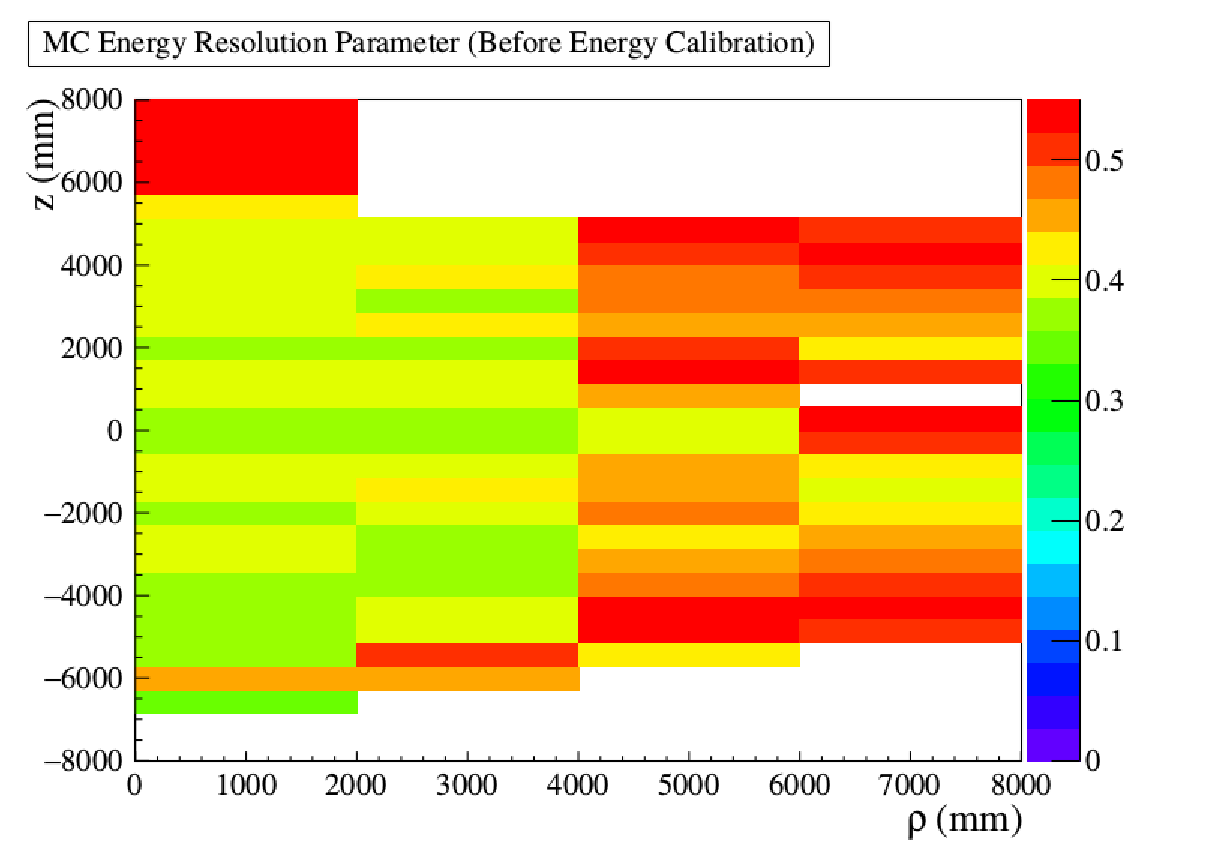
\includegraphics[width=\textwidth]{mc_sig_uniformity}
\caption[]{}
\end{subfigure}
\caption[Position Depedence of Energy Scale and Resolution from $\ce{^{16}N}$]
{The best fit energy scale before for detected (a) and monte-carlo simulated (b)  $\ce{^{16}N}$
events as a function of position.
And the best fit energy resolution parameter for detected (c) and 
simulated (d) $\ce{^{16}N}$ events}
\label{fig:n16_uniformity}
\end{figure}

\begin{figure}[htbp]
\begin{subfigure}{0.49\textwidth}
\centering
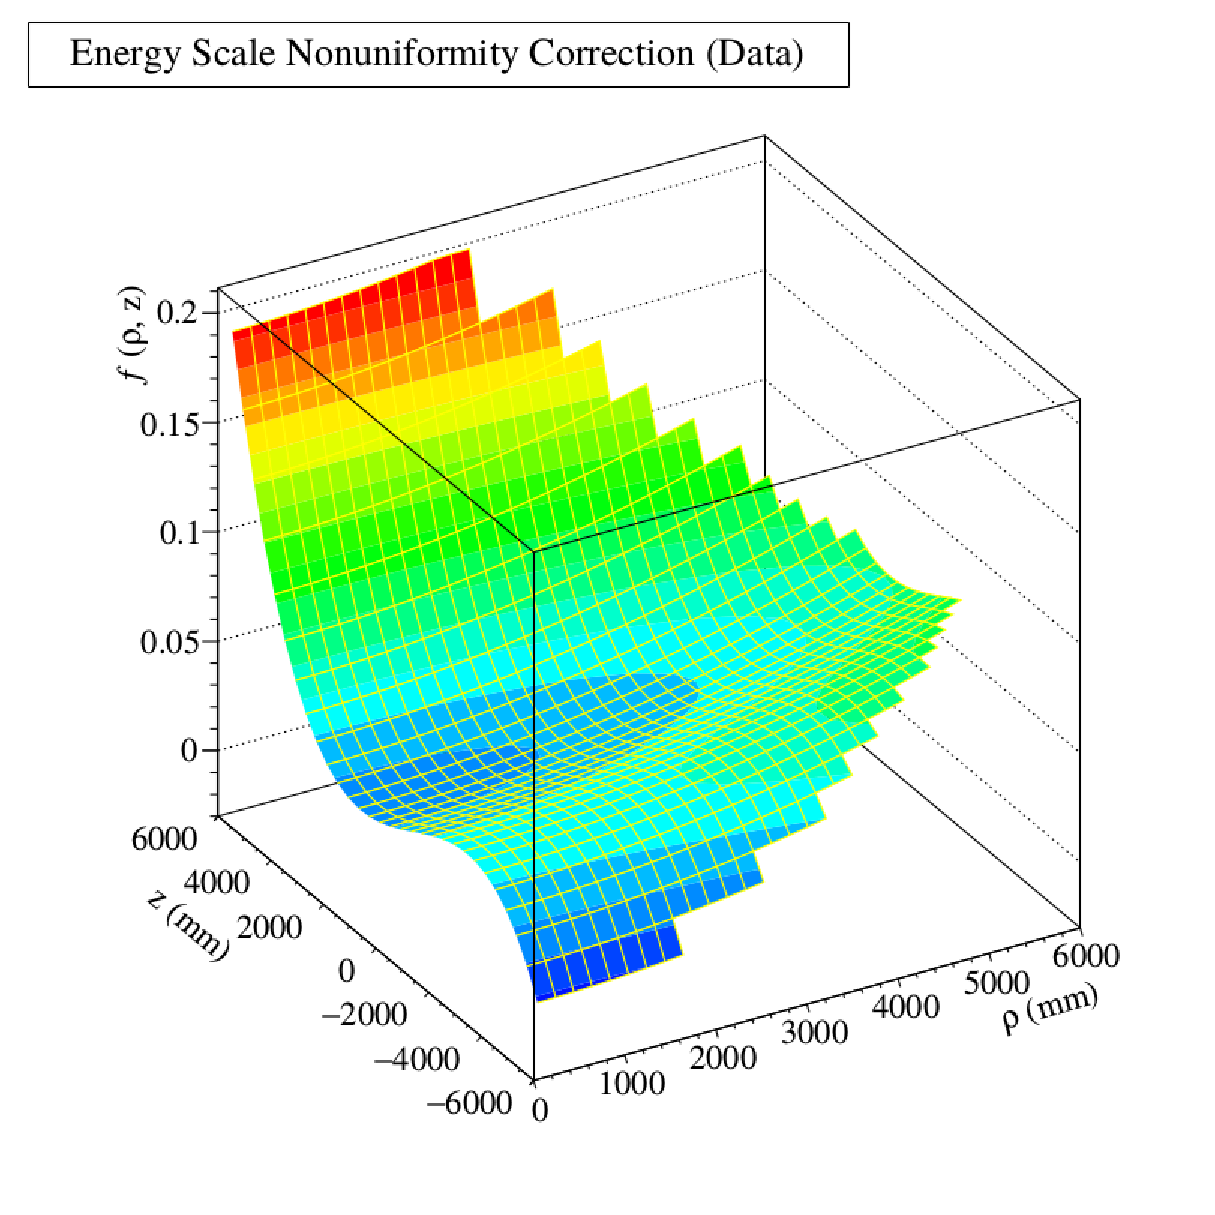
\includegraphics[width=\textwidth]{energy_uniformity_correction}
\caption[]{}
\end{subfigure}
\hfill
\begin{subfigure}{0.49\textwidth}
\centering
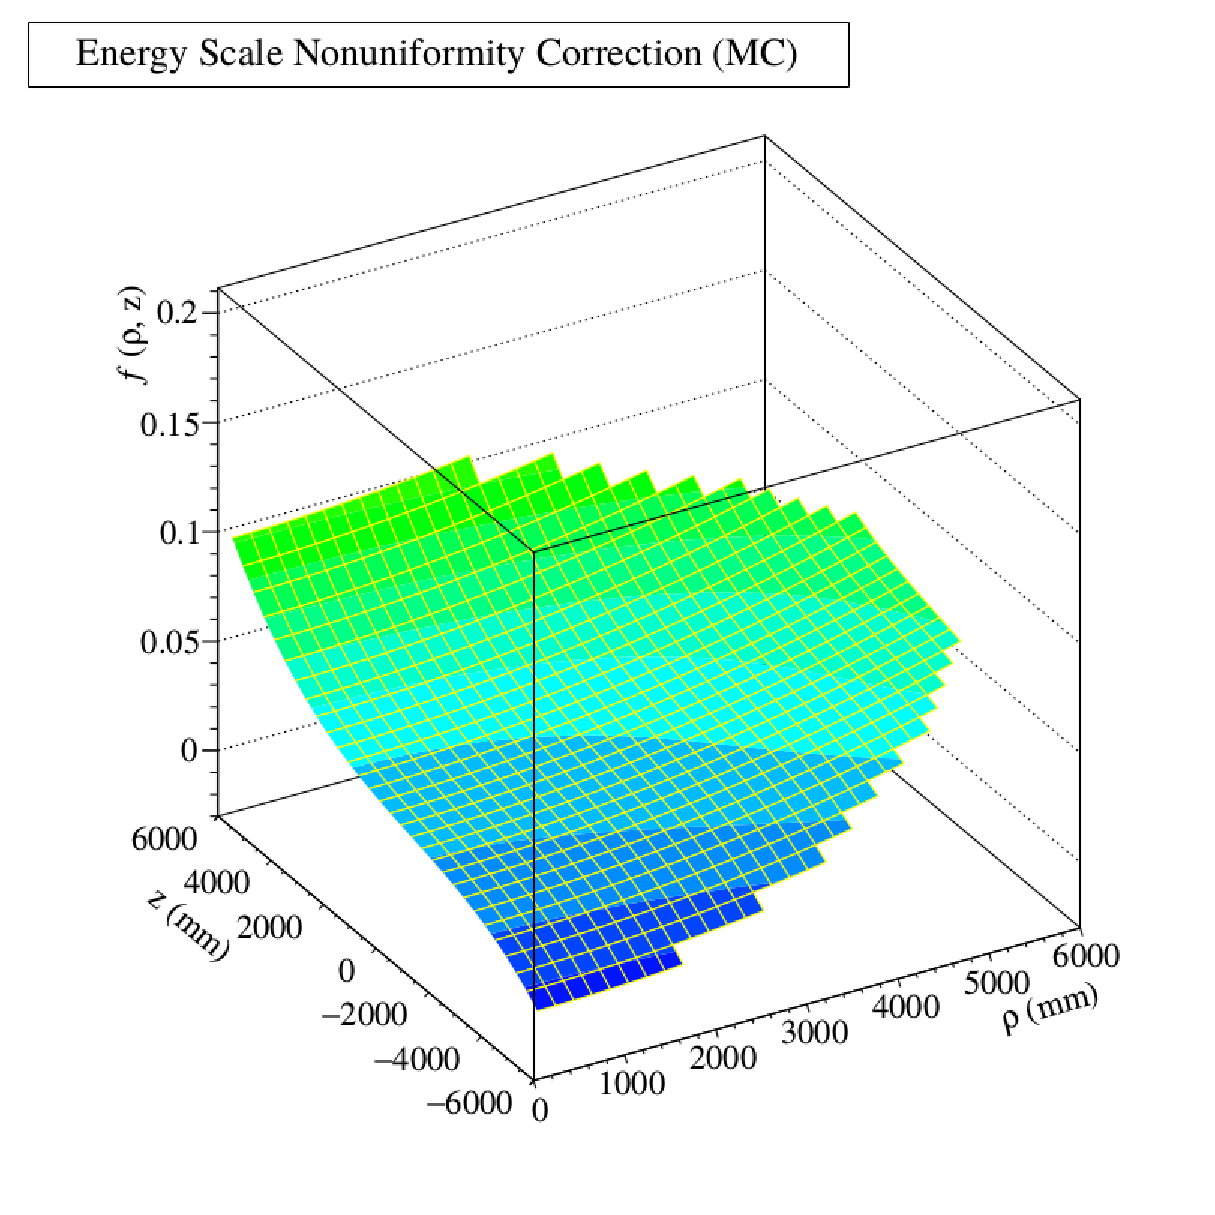
\includegraphics[width=\textwidth]{energy_mc_uniformity_correction}
\caption[]{}
\end{subfigure}

\begin{subfigure}{0.49\textwidth}
\centering
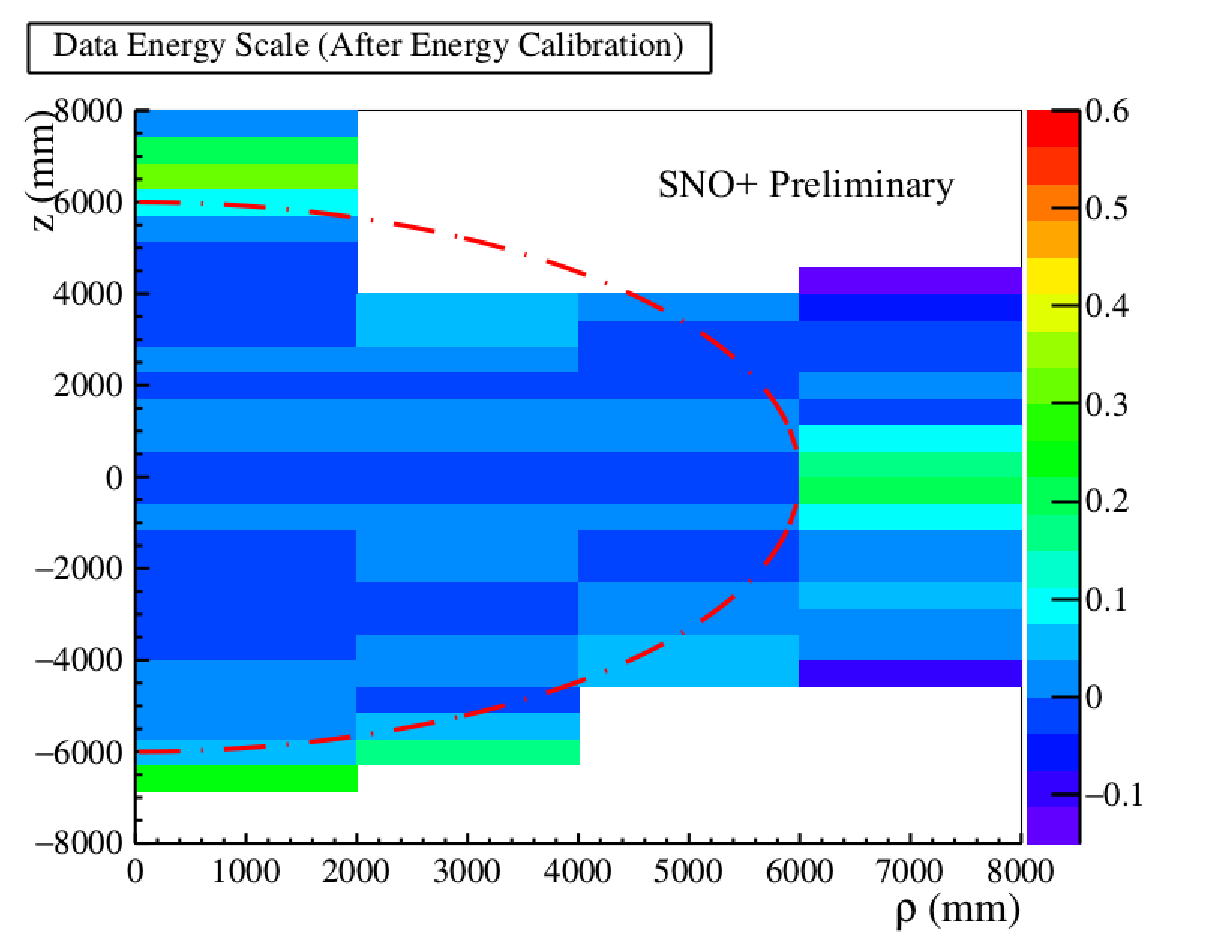
\includegraphics[width=\textwidth]{Res_data}
\caption[]{}
\end{subfigure}
\hfill
\begin{subfigure}{0.49\textwidth}
\centering
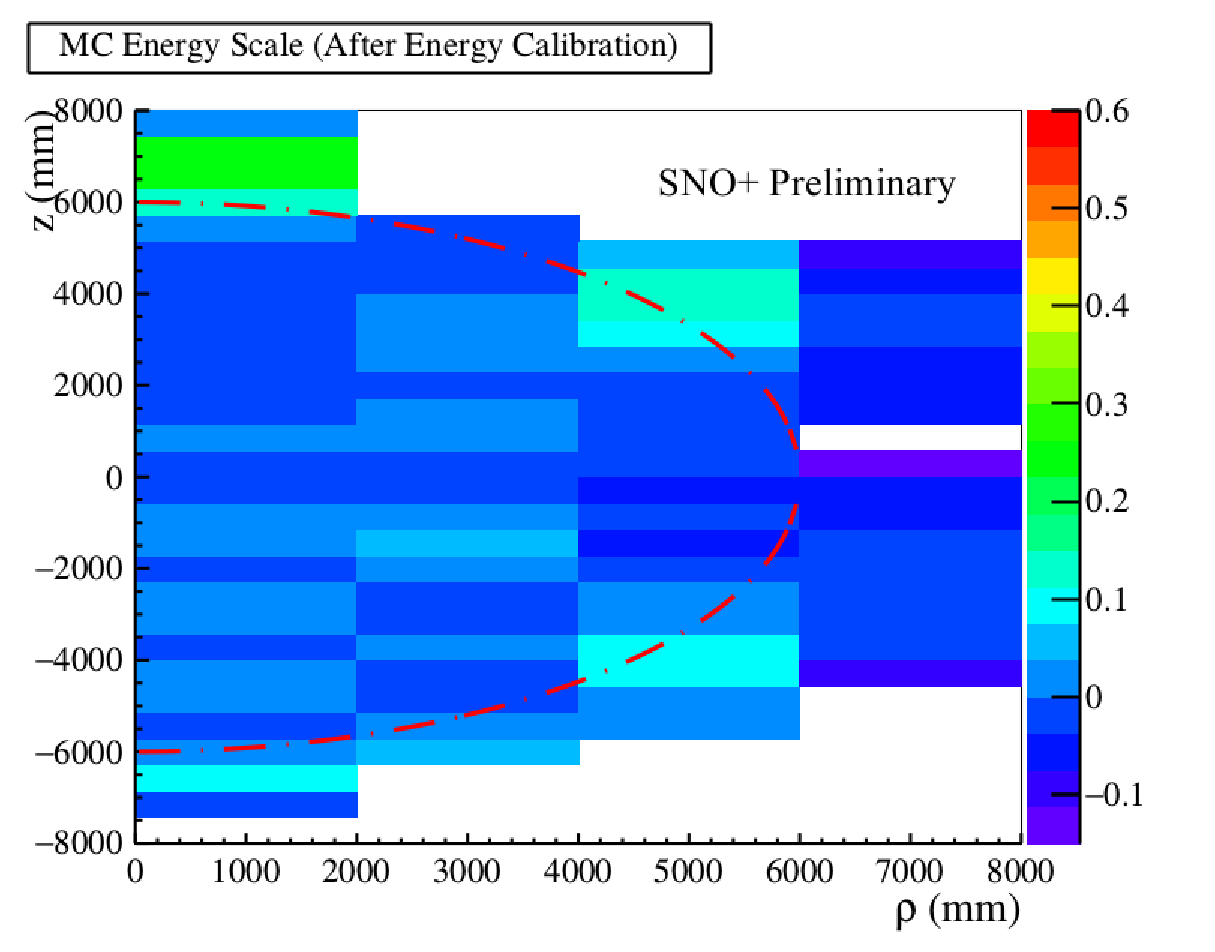
\includegraphics[width=\textwidth]{Res_MC}
\caption[]{}
\end{subfigure}
\caption[Energy Scale Uniformity Correction and Results]{The energy scale
non-uniformity correction for data (a) and MC simulation (b).
The measured energy scale as a function of position after the application
of the non-uniformity correction for data (c) and MC simulation (d).}
\label{fig:uniformity_corrections}
\end{figure}

Variations in $\delta_{E}$ along $z$ and $\rho$ were modeled by a polynomial given by,
\begin{equation}
    \delta_{E}(\rho^{2}, z) = A + \left[(1+B\rho^{2})(1+Cz+Dz^{2}+Ez^{3}) - 1\right]\text{.}
    \label{eqn:escale_position_dependence}
\end{equation}
Values for $A$, $B$, $C$, $D$, and $E$ are extracted from a fit to the observed
spatial variation of $\delta_{E}$ for simulation and data and are given in
table~\ref{tbl:n16_position_escale}.
The reconstructed energies of simulated and detected 
events are then corrected according to~\eqref{eqn:escale_position_dependence} by
their respective best fit values.
Figure~\ref{fig:uniformity_corrections} shows the correction as a function of
position in the detector and the energy scale measured across the detector
after the application of the correction.
The energy resolution is evaluated as a function of position but no correction
is determined from it.
\begin{table}
    \centering
\begin{tabular}{|c | c | c | c |c|c|}
\hline
& A&B&C&D&E\\
\hline
Data& 2.53e-2& 1.48-e9 & -5.44e-6 & 2.14e-9 & 6.49e-13\\
Simulation& 3.33e-2& 9.48e-10& 3.77e-6& 4.46e-10& 1.43e-13\\
\hline
\end{tabular}
\caption{Best fit values for~\eqref{eqn:escale_position_dependence} for
simulated and detected data, determined using units of mm for $z$ and $\rho$.}
\label{tbl:n16_position_escale}
\end{table}

After the correction is applied to remaining half of the calibration dataset
$\sigma_{E}$ and $\delta_{E}$ are determined once more as a function of position.
The bin-by-bin differences in $\sigma_{E}$ and $\delta_{E}$ between
simulated and detected data are taken as the systematic uncertainty for those
parameters, with additional fit uncertainties added in quadrature.
Averaging the bin-by-bin systematic uncertainty over the detector volume relevant
for the solar analysis yields a $2.5\%$ uncertainty on $\delta_{E}$ and an
$11\%$ uncertainty on $\sigma_{E}$.

\subsection{Position Calibration}
Similar to the energy calibration, the position reconstruction is evaluated
using $\ce{^{16}N}$ data and simulation.
The difference between the source position and the reconstructed
position of each event is determined and histogrammed.
A fit to that distribution is performed using a model of a Gaussian distribution
with exponential tails convolved with a distribution for the first gamma interaction
distance. The equation for this is given by,
\begin{equation}
    P(x)  = A \cdot \bigg[ \bigg(\frac{1 - \alpha}{\sqrt{2\pi}\sigma}e^{- \frac{(x-\mu)^2}{2\sigma^2}} + \frac{\alpha }{2 \tau}e^{-\frac{|x-\mu|}{\tau}}\bigg) \circledast P_{\gamma}(x) \bigg]\text{.}
    \label{eqn:n16_position_model}
\end{equation}
Where $\mu$ and $\sigma$ are respectively the center and width of the Gaussian,
$\tau$ represents the decay rate for the exponential tails, and $\alpha$ represents
the relative strength of the exponential~vs.~the Gaussian;
$P_{\gamma}(x)$ is distribution of distance travelled by an $\ce{^{16}N}$
gamma before it's first interaction, it is determined from a separate MC
simulation.
Finally $A$ is an overall normalization to account for the number of events
included in the distribution.
The Gaussian and exponential portion of
\eqref{eqn:n16_position_model} represents the spread introduced by the detector
and position reconstruction, the $P_\gamma$ term represents the intrinsic spread
in interaction positions from the source itself.
The distribution used for $P_\gamma$ in show in Fig~\ref{fig:gamma_first}
Figure~\ref{fig:n16_position_comparison} shows a comparison between data
and monte-carlo simulation for reconstructed position and an example fit to the data
for a central $\ce{^{16}N}$ dataset.
\begin{figure}[htbp]
    \centering
    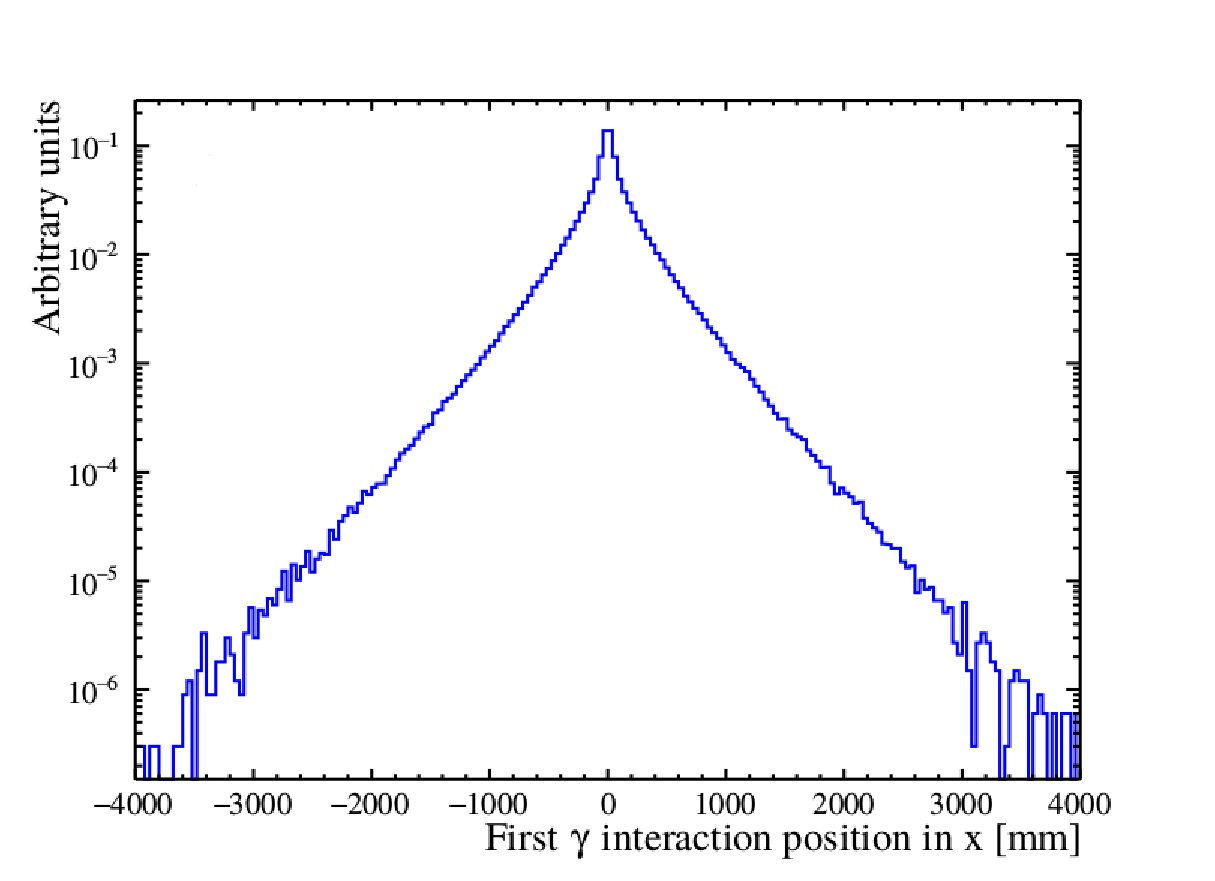
\includegraphics[width=0.79\textwidth]{gamma_first_scattering}
    \caption[Distribution of Gamma First Interaction Distance]{
    The distribution of first interaction distances for gamma ray produced
    in the $\ce{^{16}N}$ source. Produced from MC simulation and used in
    Eqn.~\eqref{eqn:n16_position_model}.}
    \label{fig:gamma_first}
\end{figure}

\begin{figure}[htbp]
\centering
    \begin{subfigure}{0.49\textwidth}
        \centering
        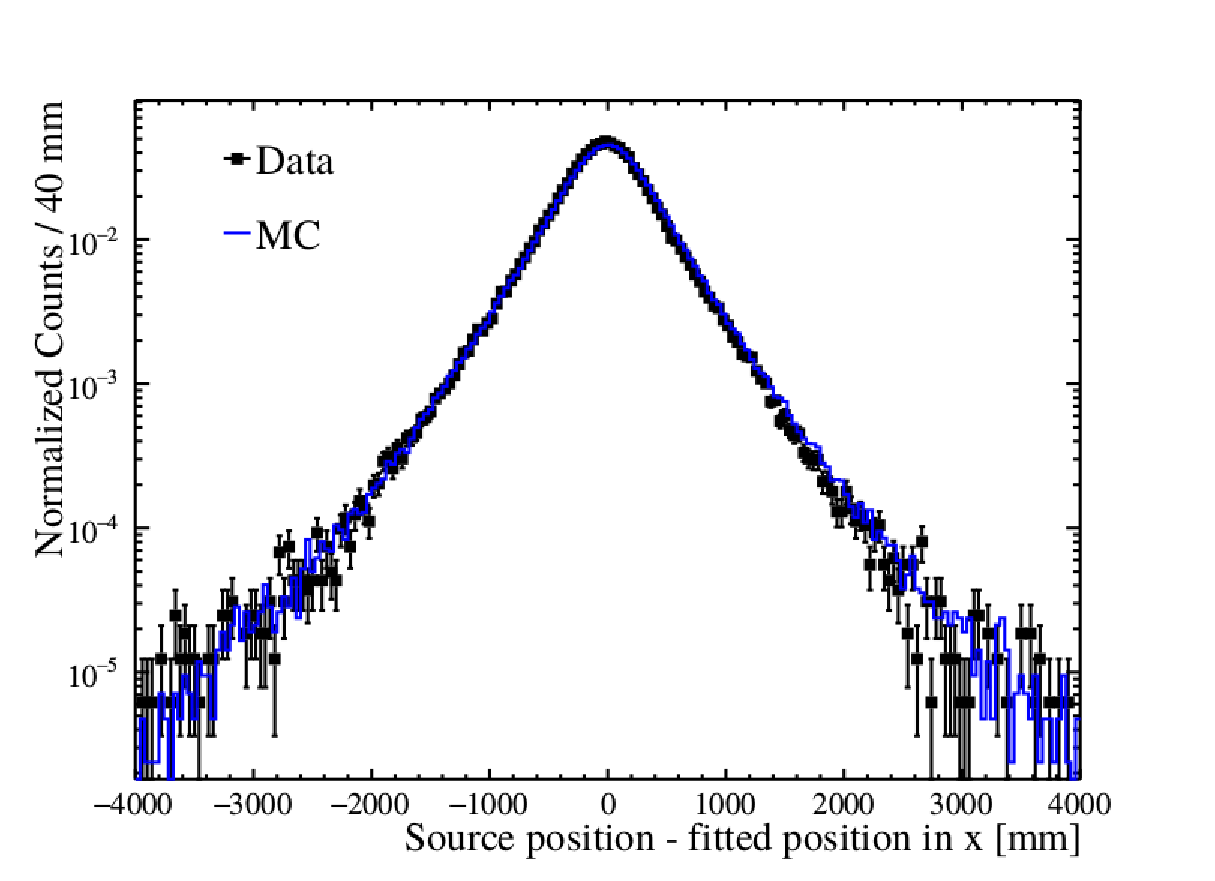
\includegraphics[width=\textwidth]{Position_data_vs_mc}
        \caption{}
    \end{subfigure}
    \begin{subfigure}{0.49\textwidth}
        \centering
        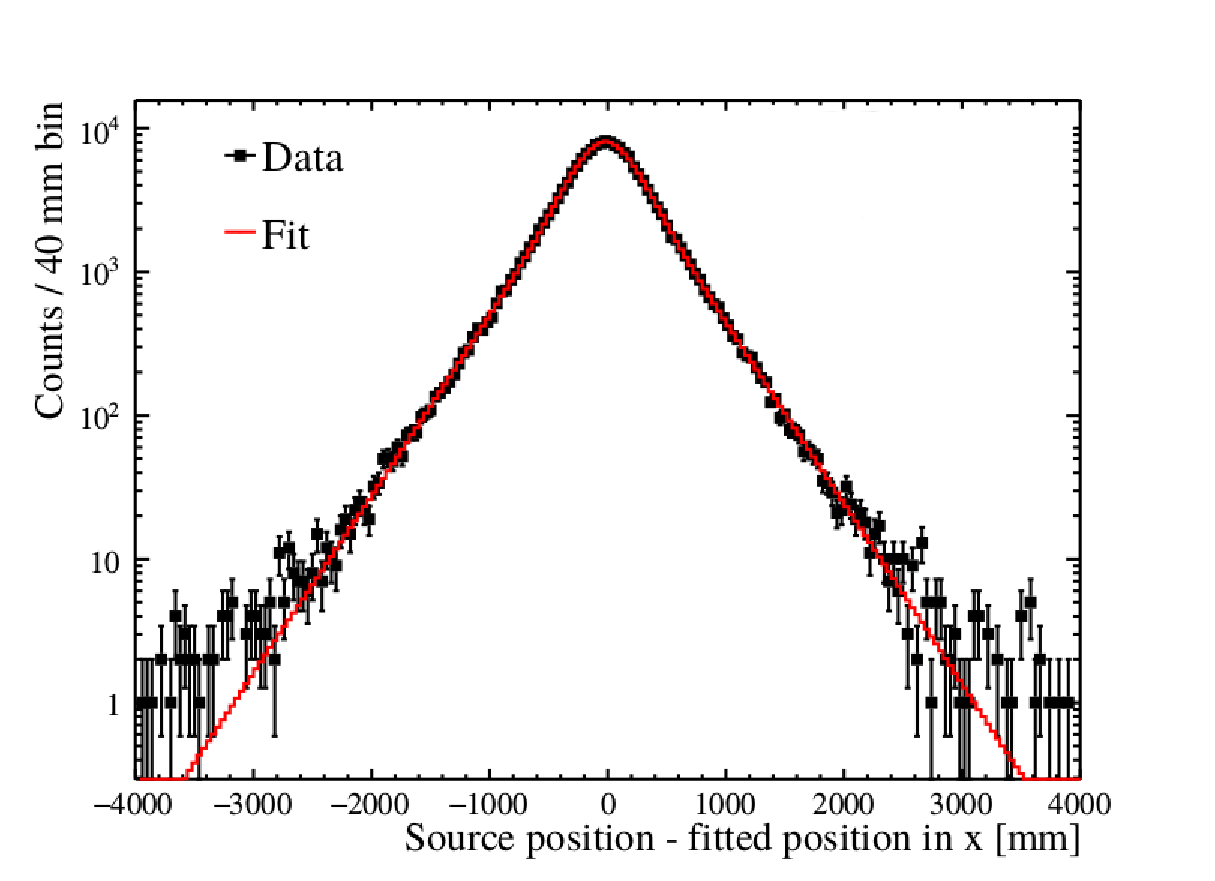
\includegraphics[width=\textwidth]{n16_position_fit_example}
        \caption{}
    \end{subfigure}
\caption[Reconstructed Postion for $\ce{^{16}N}$ events, Data and MC]{
    (a) Reconstructed position of $\ce{^{16}N}$ detected events and MC simulated
    events for a central $\ce{^{16}N}$ run. (b) An example fit to detected events,
    also for a central $\ce{^{16}N}$ run.}
\label{fig:n16_position_comparison}
\end{figure}

With this model three types of position uncertainties are considered, a shift
uncertainty, a resolution uncertainty, and a scale uncertainty.
Here a position shift is the value for $\mu$ in equation~\eqref{eqn:n16_position_model}
averaged over the entire detector volume, $\langle \mu \rangle$;
the position shift systematic then is the difference in $\langle \mu \rangle$
from MC simulation and as determined by detector data.
Rather than averaging over all source positions $\langle \mu \rangle$
is determined averaging over scans along the $x$, $y$ and $z$ axis and
so a position shift for each axial direction is determined.
Only source positions along each axis are used to avoid possible correlations
in each direction's position shift. The resulting systematic uncertainties along
each axial direction are given in table~\ref{tbl:position_shift_systs}.
\begin{table}
    \centering
    \begin{tabular}{|c|c|}
            \hline
            &$\langle \mu \rangle$ Systematic Uncertainty (mm)\\
            \hline
            x&+16.4, -18.2\\
            y&+22.3, -19.2\\
            z&+38.4, -16.7\\
            \hline
    \end{tabular}
    \caption{Position shift systematic uncertainties}
    \label{tbl:position_shift_systs}
\end{table}

The position resolution systematics is evaluated in a similar way as the position
shift systmatic, comparing values for
$\sigma^{2}$ in equation~\eqref{eqn:n16_position_model} instead of $\mu$,
but otherwise following the same procedure.
Table~\ref{tbl:position_resolution_systs} gives the extracted position resolution systematics uncertainties
in $\text{mm}$. The uncertainties are given as one-sided because a resolution uncertainty,
unlike the shift uncertainty,
can only be applied to MC simulation by applying addition smearing.
\begin{table}
    \centering
    \begin{tabular}{|c|c|}
            \hline
            &$\langle \sigma \rangle$ Systematic Uncertainty (mm)\\
            \hline
            x&104.0\\
            y&98.2\\
            z&106.2\\
            \hline
    \end{tabular}
    \caption{Position resolution systematic uncertainties}
    \label{tbl:position_resolution_systs}
\end{table}


The final position systematic considered is the position scale uncertainty,
which represents any position depended shift in $\mu$ between simulation
and data. Unlike the previous two uncertainties this systematic can effect the
number of events that would be predicted to fall within a volume if the
events are distributed uniformly throughout space. For this reason the position
scale systematic is sometimes called the fiducial volume systematic.

The position scale for simulation and data is determined by fitting the values
of $\mu$ as a function of position, along each axis, with a linear function.
The best fit slope for that line gives the position depedence of the position
shift. The value for that shift is defined to be zero at the center
of the detector. The position scale systematic can be though of as the
positional divergence introduced by the MC simulation compared to the detector
data. Table~\ref{tbl:position_scale_systs} gives the position scale systematic
uncertainty along each axis.

\begin{table}
    \centering
    \begin{tabular}{|c|c|}
            \hline
            &Position Scale Systematic Uncertainty (\%)\\
            \hline
            x&+0.91, -1.01\\
            y&+0.92, -1.02\\
            z&+0.91, -0.99\\
            \hline
    \end{tabular}
    \caption{Position scale systematic uncertainties}
    \label{tbl:position_scale_systs}
\end{table}

\subsection{Direction Calibration}
Like position and energy, the direction reconstruction is calibrated using data
from the $\ce{^{16}N}$ source. For each $\ce{^{16}N}$ event the direction
of the gamma is estimated as co-linear with the vector from the source
position to the reconstructed event position. The dot product of that vector
with the reconstructed event direction is taken, this gives the value $\cos\theta$
for that event,
\begin{equation}
    \cos\theta = \frac{\vec{p}_{\mathrm{fit}} - \vec{p}_{\mathrm{source}}}
                {\abs{\vec{p}_{\mathrm{fit}} - \vec{p}_{\mathrm{source}}}} \cdot \vec{d}_{\mathrm{fit}}\text{.}
\end{equation}
A fit is then performed to the distribution of events in $\cos\theta$ using
the model of a double exponential,
\begin{equation}
    P(\cos\theta) = \alpha\beta_{s}\frac{e^{\beta_{s}(\cos\theta -1)}}{1-e^{-\beta_{s}}} +
                    (1-\alpha)\beta_{l}\frac{e^{\beta_{l}(\cos\theta - 1)}}{1-e^{-\beta_{l}}}\text{.}
    \label{eq:direction_model}
\end{equation}
Where $\beta_{s}$ and $\beta_{l}$ represent the ``short'' and ``long'' decay constants
for the two exponentials, and $\alpha$ represents the relative
strength of the short exponential vs the long one.
This model was developed by the SNO experiment and is used here simply as an empirical
method to parameterize the distribution of events in $\cos\theta$.
It is shown in~\citep{pierre_luc_thesis} that the systematic uncertainties on the
parameters derived from~\eqref{eq:direction_model} can be transformed to a shift
in $\cos\theta$ given by,
\begin{equation}
    \cos\theta^{\prime} = 1+(\cos\theta-1)(1+\delta_{\theta})\text{,}
\end{equation}
where $\delta_{\theta}$ is the relative systematic uncertainty of $\beta_{s}$ and $\beta_{l}$.
Transformed this way the systematic uncertainty for the direction reconstruction
is given by
\begin{equation*}
    \delta_{\theta} = +0.08\text{,} -0.13\text{.}
\end{equation*}

\subsection{Trigger Efficiecy}
The trigger efficiency for this analysis is defined to be the probability that
the detector will trigger on an event as a function of the number of ``in-time''
hits produced by that event.
Here, in-time hits is the effective maximum number of hits as seen by the analog
trigger system for an event.
For each event the in-time nhit, $\tilde{n}_{100}$, is well
estimated by the maximum number of hits in a 100\,ns window within the event.
Effects from the rise-time of trigger pulses and the limited band-width of the
trigger system are applied as corrections to that simple estimate.

The trigger efficiecy is estimated in two different ways, using laserball
data, and using nhit-monitor data.
These methods disagree by a small, but non-negligible amount, the
reason for the disagreement is not well known, but the differences are taken
as a systematic uncertainty. Figure XXX shows the trigger efficiecy curves
for nhit-monitor and laserball data.

The nhit-monitor is detector calibration  process that's run periodically during
standard data taking. It simply consists of sending a variable number
of pedestal hits to the front-end, and then observing if the detector triggers
off of those hits or not. For the entierty of the dataset only channels in
crate 4 of the detector were pedestalled for the nhit-monitor.
This is one reason to prefer the trigger efficiency curve provided by laserball
data, the hits from the laserball are isotropic and present a much lower risk of
over-sampling a small number of channeles in the detector. Although all channels
in the detector are designed function identically, this is not something that
is closely monitored or tested, so it could be the case that the channels on
crate 4 are not represetative of the detector as a whole.

For runs taken after the detector threshold change discussed in Sec~\ref{XXX}
all methods agree that the trigger is 100\% efficient for $\tilde{n}_{100} > 10$;
only events with energy significantly below the analysis threshold (discussed
in Section~\ref{XXX}) will have a $\tilde{n}_{100} \le 10$, and so the discrepannt
estimates of the trigger
efficiecy do not have any effect on the solar analysis for the second trigger period.
For the first trigger period the trigger was not 100\% efficient till
$\tilde{n}_{100} \approx 23$, which is much closer to the analysis energy
threshold, and therefore uncertainties cannot be neglected.

%\section{Blindenss}
%The majority of this analyses was designed with the data blinded in the
%relevant energy region.
%The data blinding was done primarily for a nucleon decay analysis~\citep{snop_nd}
%that was performed using the same dataset as this analyses, but was done
%for this analysis as well because both results were produced contemporaneously.
%
%%TODO check these numbers
%The scheme for blinding the data was to remove all events from the dataset that
%had an nhit between $30$ and $100$, this correspond to an approximate electron energy
%range of \numrange{4.0}{15.0}\,MeV.
%The analyses was designed primarily using simulation and a two-week open
%data period, on which no blindness restrictions were imposed.
%
%Part way through the analysis testing and design the data was partially un-blinded
%to allow for an initial look at the results.
%Blinded events that reconstructed energy between $4.5$\,MeV and $15.0$\,MeV
%were added into the dataset with all energy related information removed;
%each event was assigned the artificial energy of $10.0$\,MeV.
%With those data, plots of the distribution of event direction with respect to
%the sun were created and provided a check that the results were as expected.
%The energy cut used to select events for that plot was performed using
%un-calibrated energy, so it has little bearing on the results of the full
%analysis.

\section{Data Selection}
\label{sec:data_selection}
Events are included or removed from the dataset across three stages of selection.
First entire runs are either included or removed based upon whether they meet
certain criteria for data quality.
The events within selected runs are then rejected or approved by a set
of low-level cuts that attempt to remove events caused by instrumental
backgrounds and other sources of unwanted events.
Within events that pass the low-level cuts, hits can be rejected from consideration
if they're deemed unlikely to have originated from light within the detector.
Following that, analysis level cuts are applied to the reconstructed quantities
for each event.
The analysis cuts are designed to maximize the signal efficiency for dataset and minimize the
contamination from background sources.
Each of these steps are detailed below.

\subsection{Dataset}
\label{sec:dataset}
Data for this analysis was taken in SNO+'s initial water-phase data-taking
run.
Data taking started May 05 2017 (exactly 4 years after I
started my PhD) and ended December 25 the same year.
The data taking started with run $100000$ and concluded with run
$108416$, with each run being typically 1 hour long, though not
all runs are suitable for analysis.
In those runs approximately 185 days worth of useable data was taken,
with significant pauses for commissioning of ancillary detector components,
such as the water circulation systems, and for detector maintenance.
Data taking was restarted several months after the end of this dataset,
after the AV circulation pipes had been replaced to help reduce backgrounds
in the detector.

In the dataset there are a three different periods of data taking that are
given special treatment in this analysis
to be considered.
The first is that an external water circulation pipe was observed to have
introduced backgrounds into the upper-portion of the detector, between the
PSUP and AV\@.
For data taken during this period of time analysis cuts were adjusted, as
will be discussed in Sec~\ref{sec:analysis_cuts}.
The elevated background levels lasted from run $100400$ to $102048$.
These runs are referred to as the ``hot-spot'' runs.

The other period of time that requires special treatment within the analysis
is due to significant adjustments to the detector trigger settings done approximately
half-way through the dataset.
So the dataset is split into a high and low trigger period, the high trigger
period being first.
The high trigger period started at run 100000 the low trigger period started
at run 104613.
The adjustment made was to raise the threshold on all channel threshold
by a single DAC count.
The result was a significant reduction in the observed dropout and noise rate
in the detector, which allowed for the trigger threshold to be pushed further
down, and an overall increase the detector's efficiency.

\begin{figure}[htbp]
    \centering
    \begin{subfigure}[b]{0.48\textwidth}
        \centering
        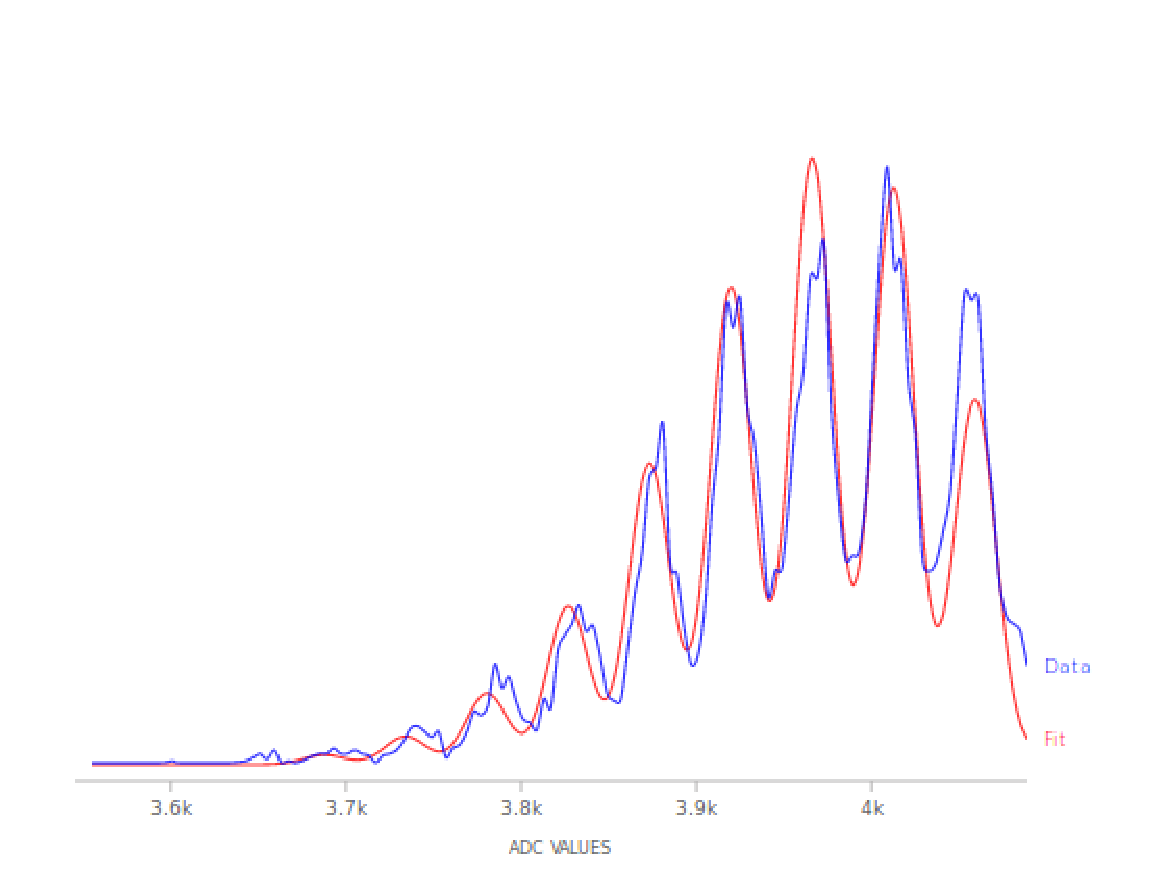
\includegraphics[width=\textwidth]{pre_trigger_dropout}
        \caption[]{}
    \end{subfigure}
    \hfill
    \begin{subfigure}[b]{0.48\textwidth}
        \centering
        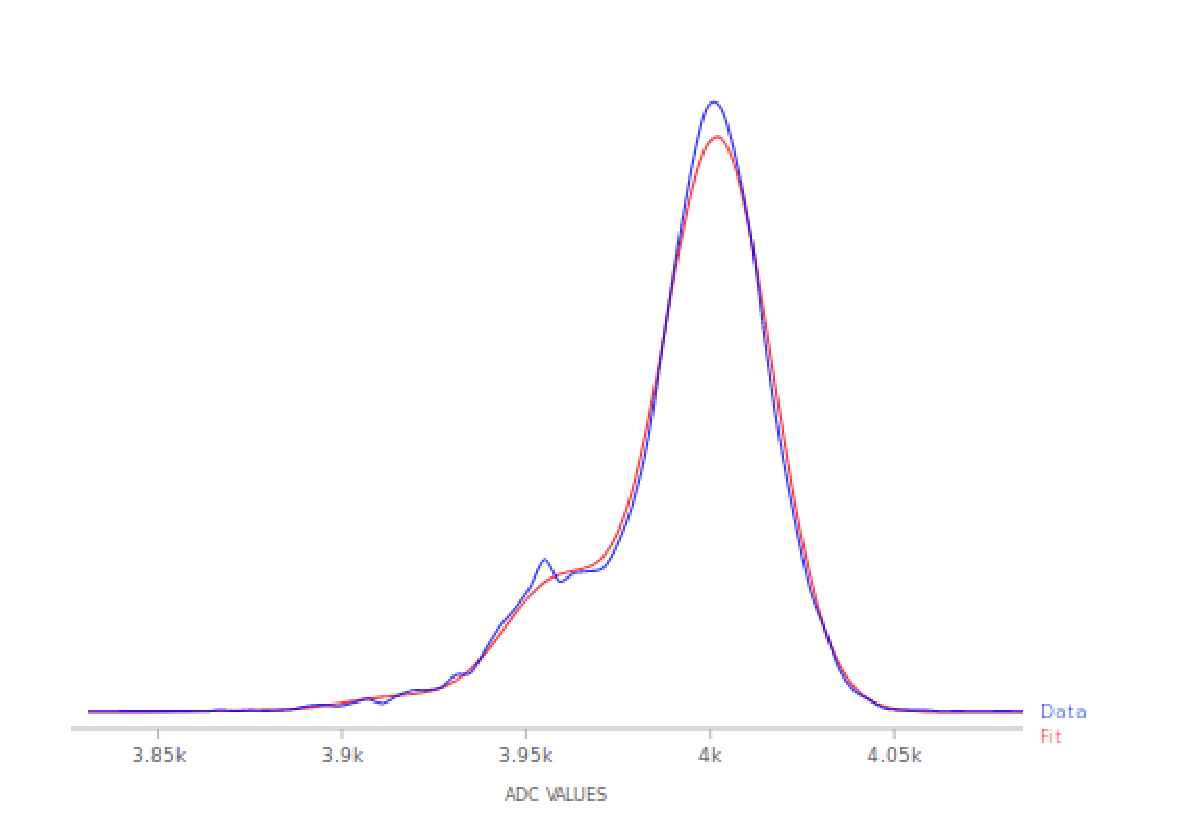
\includegraphics[width=\textwidth]{post_trigger_dropout}
        \caption[]{}
    \end{subfigure}

    \begin{subfigure}[b]{0.78\textwidth}
        \centering
        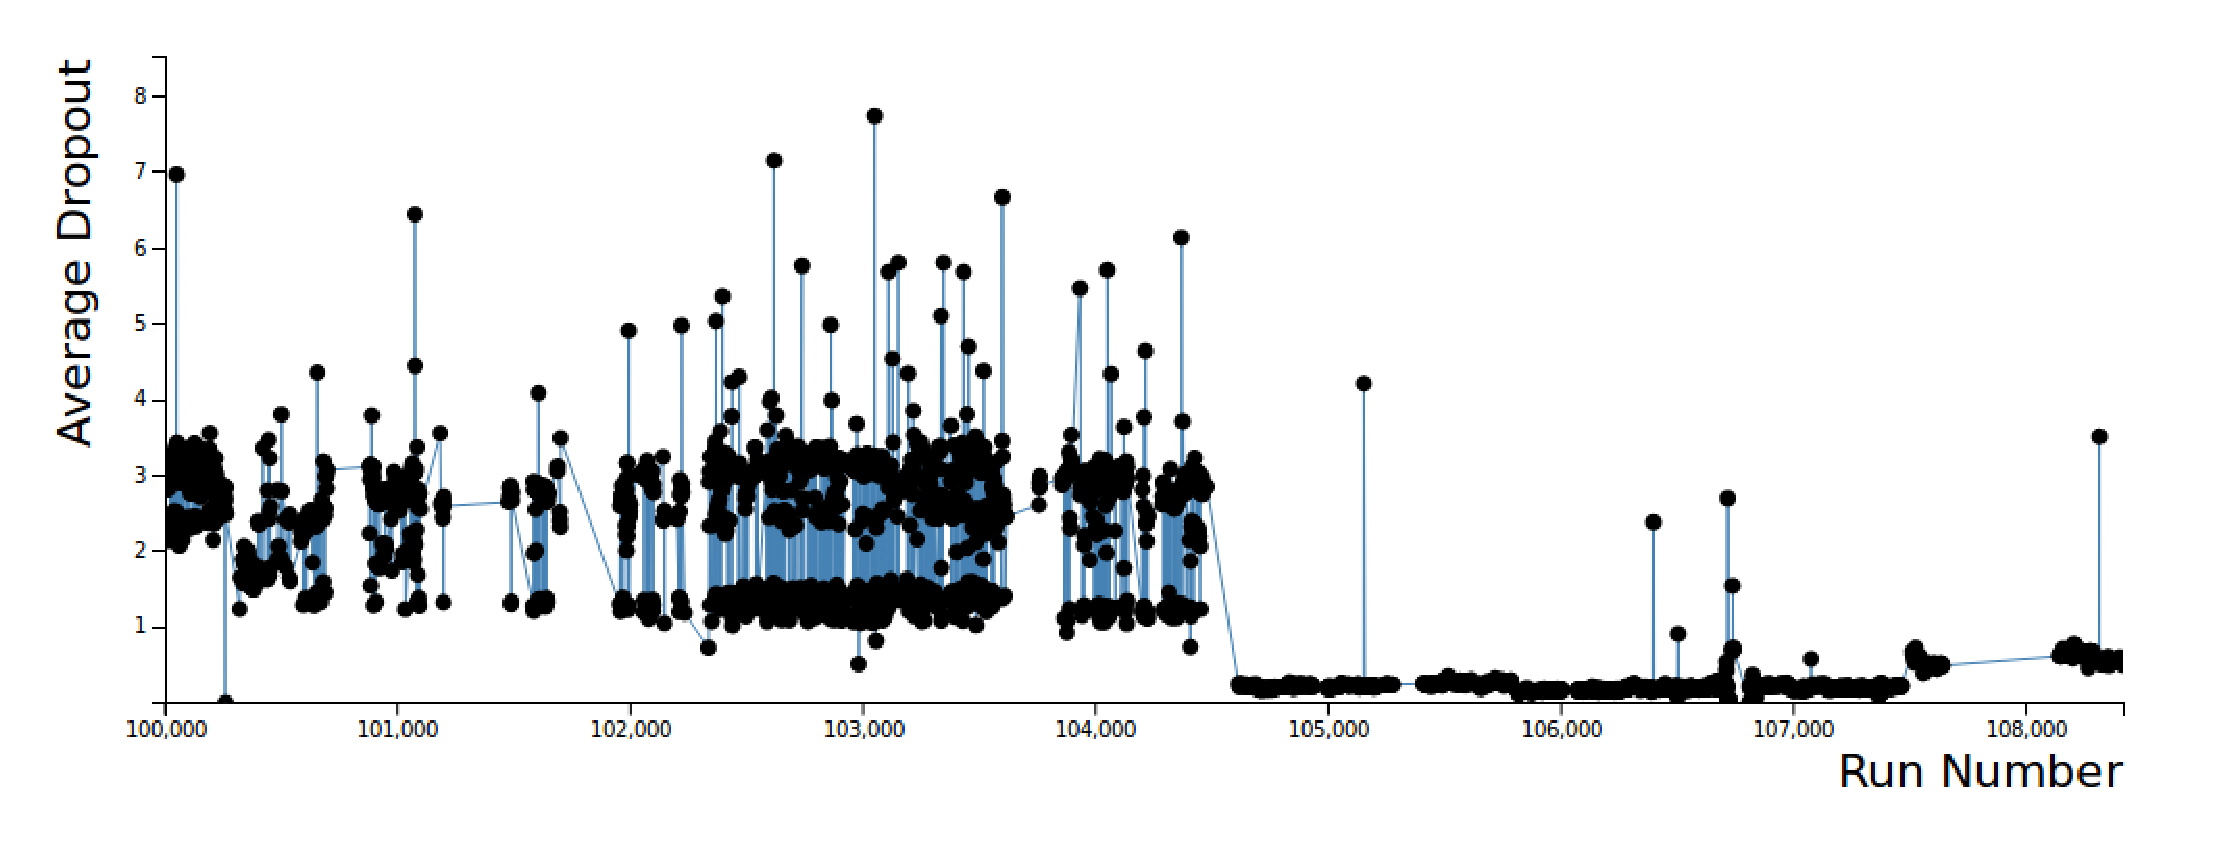
\includegraphics[width=\textwidth]{dropout_nd}
        \caption[]{}
    \end{subfigure}
    \caption[Dropout In Low and High Trigger Period]{
        N20 dropout in the high (a) and low (b) trigger period,
        and the average dropout measured across all runs in the
        dataset (c); the various ``jumps'' in the dropout are generally
        due to bad fits.}
    \label{fig:dataset_dropout}
\end{figure}

It's not known why the adjustment to channel thresholds resulted in such a significant
reduction in the noise.
It may be the case that adjusting the threshold reduced the rate of dropout.
Figure~\ref{fig:dataset_dropout} shows a dropout measurement before and after the trigger
adjustment, which shows how significant the dropout rate reduction in the trigger
system was.
It's not known if the in dropout is a side-effect of the noise reduction in
the system, or the cause of it.

\subsection{Run Selection}
\label{sec:run_selection}
Runs are rejected from the dataset if they fail to meet certain criteria
for data quality and detector stability.
It's first required that all meta-info about a run be created and stored
within the RAT Database successfully.
Those tables have information about the state of the hardware and DAQ, as
well as information about the run including the run type and length.
This information is necessary for assessing if the run is capable of being
used for a physics analysis.
It's further necessary that all meta-info be available so that the run
can be simulated.
It's very rare for the meta-info for a run not to be generated and stored
properly, so this check has a almost no effect on the dataset.

It's required that the run type of the run be ``PHYSICS'', this indicates
that the DAQ settings were not changed at any point in the run and no external
sources of events were present, and that the thresholds for triggering were set
at a level deemed sufficient for most physics analyses.
Following this checks are done
that require all electronics crates have high voltage on their PMTs throughout
the run.
It's also required that all channels that are at high voltage are capable of
reading out data, and that all crates are participating in the trigger sums.
A number of separate checks are performed to ensure that all necessary DAQ
processes were running well throughout the run, to ensure that the data taken
during the run was not interrupted by a lapse in the DAQ.\@

Beyond checks on the detector state and stability, a number of checks
are placed on the data taken within the run.
Most of these checks are placed on the rate of certain events within the detector.
It's required that the ESUMH and N100L trigger rate be greater than 5Hz and
that the total trigger rate be less than 7kHz.
These checks ensure that the data taken during the run triggered the detector
at a rate consistent with standard running, during which the typical trigger
rate is near 1kHz.
Similarly it's required that fewer than 15\% of all events be retrigger events
(events that fall within 420\,ns of the previous event).
At a nominal rate of 1kHz it's very unlikely for two event to be within $420$\,ns
by chance, so a high rate of retrigger events might indicate a high level
of noise in the trigger hardware. There are however events that can occur
in the detector, such as followers after a cosmic muon, that can produce
re-trigger events.
The cut threshold is designed to allow for retriggers from natural source but
still flag detector abnormalities.
These checks all ensure that the data in a run is likely to be useful for
a physics analysis, but are loose enough not to bias the dataset in a way that
might influence results.

\subsection{Livetime}
While most event selection removes individual events based upon whether they
pass or fail certain criteria, some cuts remove all events that occur for a
period of time before or after some criteria is met.
These cuts are said to introduce a deadtime into the dataset.
The most significant example of this is the muon follower data cleaning cut, which
cuts all events for 30\,seconds after every muon interaction in the detector.
The livetime for each run is then defined as
\begin{equation}
    t_{\mathrm{live}} = t_{run} - t_{\mathrm{dead}}\text{,}
\end{equation}
where $t_{run}$ is the time between the first and last valid event within a run
and $t_{\mathrm{dead}}$ is the sum of all deadtimes introduced into that run by cuts.
The livetime is used to calculate the total exposure represented by the dataset.
For simulated events many of the effects that necessitate deadtime are not simulated,
so no deadtimes are added into the simulated runs.
%Table XXX shows the sum of deadtimes across all runs within the dataset.
The livetime represented by the dataset is 120.2 days, after subtracting the
calculated deadtimes the effective livetime  114.7 days.

\subsection{Data Cleaning}
There are a number of instrumental effects that can cause an event
to be recorded by the detector, these events typically have some
sort of distinguishing feature or features that set them apart
from events that originate from particle interactions within the
detector.
A number of algorithms and cuts have been designed to identify and remove
these events from the dataset.
These algorithms are said to ``clean'' the data by removing events
of instrumental origin. These definition is extended to include removing
hits within an event that are likely of instrumental origin as well.

The primary type of instrumental event that must be removed is ``flashers'' and
``shark-fin'' events.
Both of these result from charge build-up on the PMT-base causing a
spark.
For a flasher event the light from the spark escapes through the PMT face
and illuminates the PMTs on the other side of the detector.
Flashers occur at a rate of a few per minute.
A shark-fin is similar but the spark is either small enough or located
in a position such that the light does not escape the PMT.\@
In both types of events the PMT in which the spark occurs with readout
a very high-charge hit, and the channels next to it on the FEC will
have low-charge hits from electronic pickup.
For shark-fin event no other channels will be hit, except possibly by an
accidental coincidence; for a flasher hit a number of hits will
occur from the light that escaped the PMT.\@
Since the number of PMT hits that occur in a flasher event can vary significantly,
anywhere between tens of hits and hundreds, they can reconstruct
to a wide range of energies and possibly contaminate a signal region.
Many data cleaning cuts are designed to ensure that all
flasher events are identified and removed from the dataset.

Within an event hits that are deemed unlikely to have come from a photon interacting with a PMT
are removed from the analysis through hit cleaning.
For this analysis the only sort of hits that were removed were those identified
as coming from cross-talk between adjacent channels in the detector.
Hits from cross-talk arise from stray capacitative coupling between adjacent, or nearby, channels
on a single daughter board.
Typically the noise from cross-talk will only be large enough to cause a hit
on adjacent channels if the original signal is relatively large.
The cross-talk hits will usually be especially low in charge because they're
the result of bi-polar noise, rather than a PMT signal, and the cross-talk
hit will always show up after the original hit.
These criteria are codified as a cut on any hits that show up within
 six channels from a hit that has a pedestal subtracted QHS greater
than 50\,ADC counts. Of those hits if it has a pedestal subtracted QHS between
$10$ and $-30$ and are between 9 and 25\,ns after the high charge hit,
then the hit is flagged a cross-talk hit and removed from the analysis.

Events of instrumental origin are not well modeled within our simulation,
so simulation is not used for evaluating the efficiencies and sacrifices of
data cleaning cuts.
Instead a data-driven approach is used that relies primarily on calibration
data from the $\ce{^{16}N}$ source, that analysis is detailed in~\citep{dc_document}.%Teals data cleaning stuff
The basic approach is to use tagged $\ce{^{16}N}$ events as a source of known
non-instrumental events, and evaluate what fraction of the time those events
are identified as instrumentals, this provides an estimate of the data-cleaning
sacrifice. The results of this analysis estimated a $1.2$\% percent signal
sacrifice from data cleaning.

An estimate of the signal contamination was performed using a method developed
by SNO~\citep{neil_thesis} and applied to the dataset~\citep{dc_document};
the number of instrumental events leaked into the signal region was estimated
to be roughly $0.5$ events over the entire dataset.
However, a contamination estimate is not an input to the solar analysis,
so that value is not used beyond a check that the instrumental background
is reduced to a acceptable level.

Each data cleaning cut is associated with a bit in a 64-bit binary value called
the data cleaning word or data cleaning mask.
The cuts that each event passes or fails is tracked by its data cleaning mask.
For the solar analyses all events are required to pass all cuts
given by the data cleaning mask \texttt{0xFB0000017FFE}.
This corresponds to the following data cleaning cuts:
    \textbf{Zero Zero Cut},
    \textbf{Crate Isotropy Cut},
    \textbf{FTS Cut},
    \textbf{Flahser Geo Cut},
    \textbf{ITC Time Spread Cut},
    \textbf{Junk Cut},
    \textbf{Muon Tag},
    \textbf{Neck Cut},
    \textbf{Owl Cut},
    \textbf{QCluster Cut},
    \textbf{QvNhit Cut},
    \textbf{QvT Cut},
    \textbf{Ring Of Fire Cut},
    \textbf{Two-Pass Muon Follower, Short},
    \textbf{Polling Cut},
    \textbf{Retrigger Cut},
    \textbf{Two-Pass Burst Cut},
    \textbf{Missed Muon Follower Cut},
    \textbf{Missing CAEN Data Cut},
    \textbf{Ped Cut},
    \textbf{Atmospheric Cut}.
Of those cuts I'll detail here the motivation behind and evaluation of the
cuts that I developed, the cuts that I did not directly develop are described in~\citep{dc_document}.

\subsubsection{Ped Cut}
During normal detector operations there are a few trigger calibration
tests that are periodically ran.
These tests use the PEDESTAL signal to inject a certain amount of fake hits
into the detector, and events with those hits are inspected to evaluate the efficiency and
quality of the trigger response.
It's very important that these events are clearly identified and removed from the
dataset so that the fake PEDESTAL hits are not confused for a real signal.
Additionally, the trigger calibration processes usually include changing settings
related to the PEDESTAL signal on the FEC, there's reason to believe these sort
of changes can introduce noise to the front-end.
So an aggressive approach of cutting all events that are within one second of
a pedestal event is used.
This not only cuts events but introduces a dead time into the dataset,
this deadtime is subtracted from the overall livetime.

\subsubsection{Missed Muon Follower Cut}
The missed muon follower cut was a data cleaning cut used in SNO, but I adapted
it for SNO+.
In SNO it was very important to identify and cut neutrons that follow
after a cosmic muon event, those neutrons could fake
a neutral current solar neutrino event.
In SNO+ this is not as much a problem because neutron captures in water will
primarily produce a $2.2$\,MeV gamma, which is below the analysis threshold for
solar neutrinos.
However, there does exist events in the dataset which are observed to follow
after high-nhit, events. The origin of these events is not well understood, they
could likely be instrumental, or from  spallation products within the detector.
Since solar neutrino events are not expected to have any time correlations
with other events in the detector, a cut can be placed on the time between
events with relatively little sacrifice.\\

The cut considers three values, an initial and a follower event nhit, $N_{1}$
and $N_{2}$, and a time difference between the two events $\Delta t$;
a threshold is placed on each of these three values, and any pairs of events that cross
each threshold are cut and so is all other events that fall within the threshold
time window.
To evaluate the cut optimal cut criteria for $N_{1}$, $N_{2}$ and $\Delta_{t}$
two different values are considered.
The first is the probability that an event of nhit greater than $N_{2}$ will occur within a time
window $\Delta t$ after an event of nhit greater than $N_{1}$.
This values is called the follower probability, $P_{F}(N_{1}, N_{2}, \Delta t)$.
The second values is the probability that an event of nhit $N$ will occur
within a time window $\Delta t$ that is chosen randomly, this value
is called accidental probability or random coincidence probability, $P_{R}(N, \Delta t)$.
Under the assumption that there is no time correlation with non-background
events the probability of this cut sacrificing a signal event is
\begin{equation}
    \mathrm{Sacrifice} = P_{R}(N_{1},\Delta t)P_{S}(N_{2}) + P_{R}(N_{2}, \Delta t)P_{S}(N_{1})\text{,}
\end{equation}
where $P_{S}(N)$ is the probability for a signal event to have an nhit above
$N$.

\begin{figure}[htbp]
    \centering
    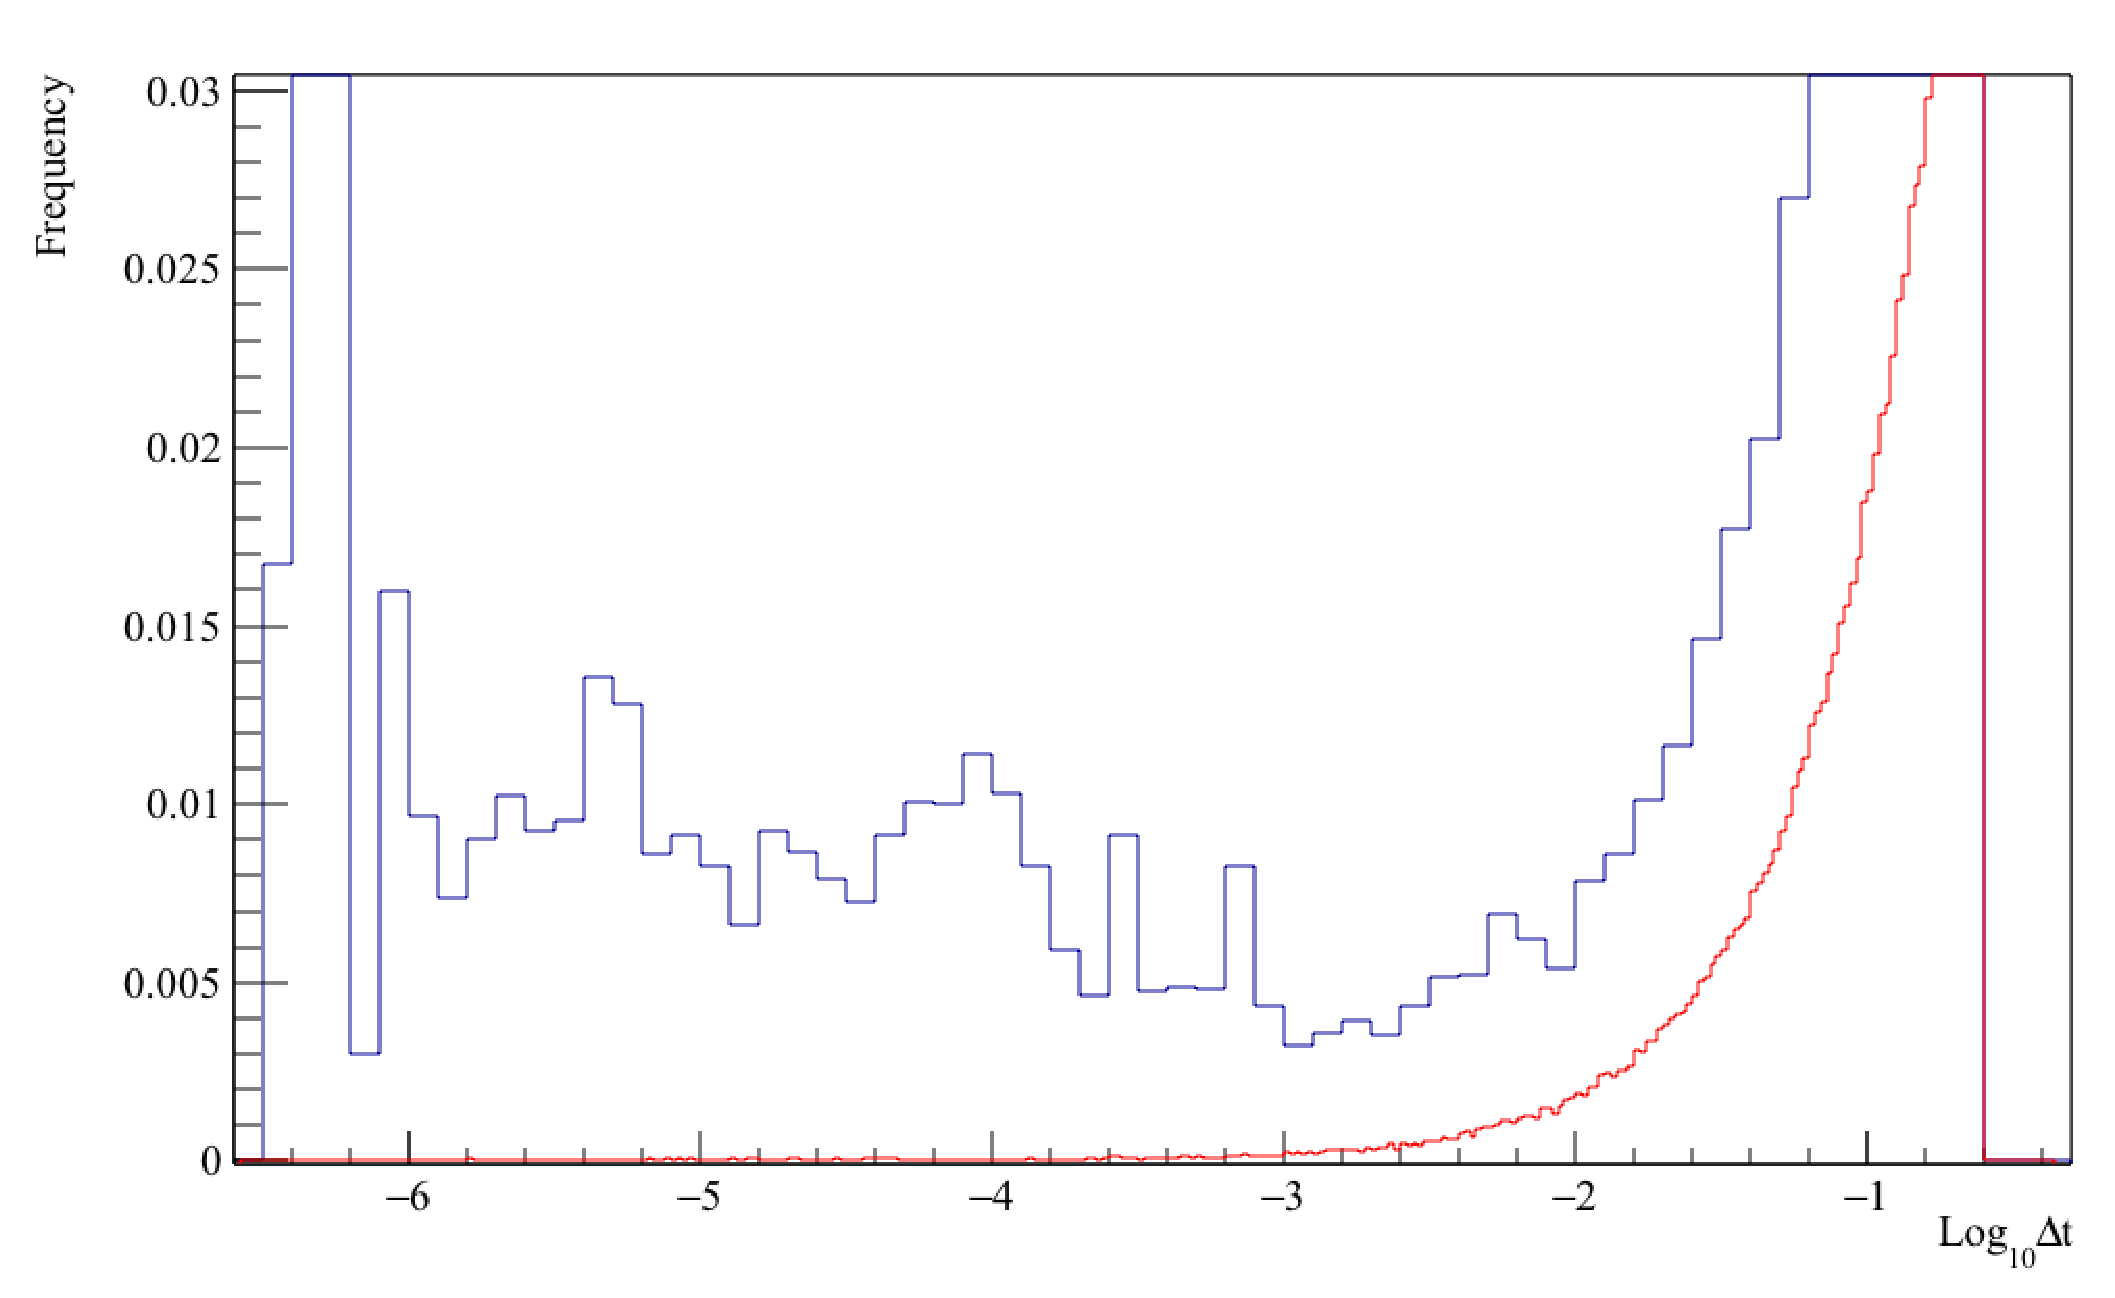
\includegraphics[width=0.74\textwidth]{mmf_pr_v_pf}
    \caption[Missed Muon Follower Example PDFs]{
        $P_R(N_2=20, \Delta t)$ (red) vs $P_F(N_1=60, N_2=20, \Delta t)$ (blue).}
\label{fig:mmf_sac}
\end{figure}
\begin{figure}[htbp]
    \centering
    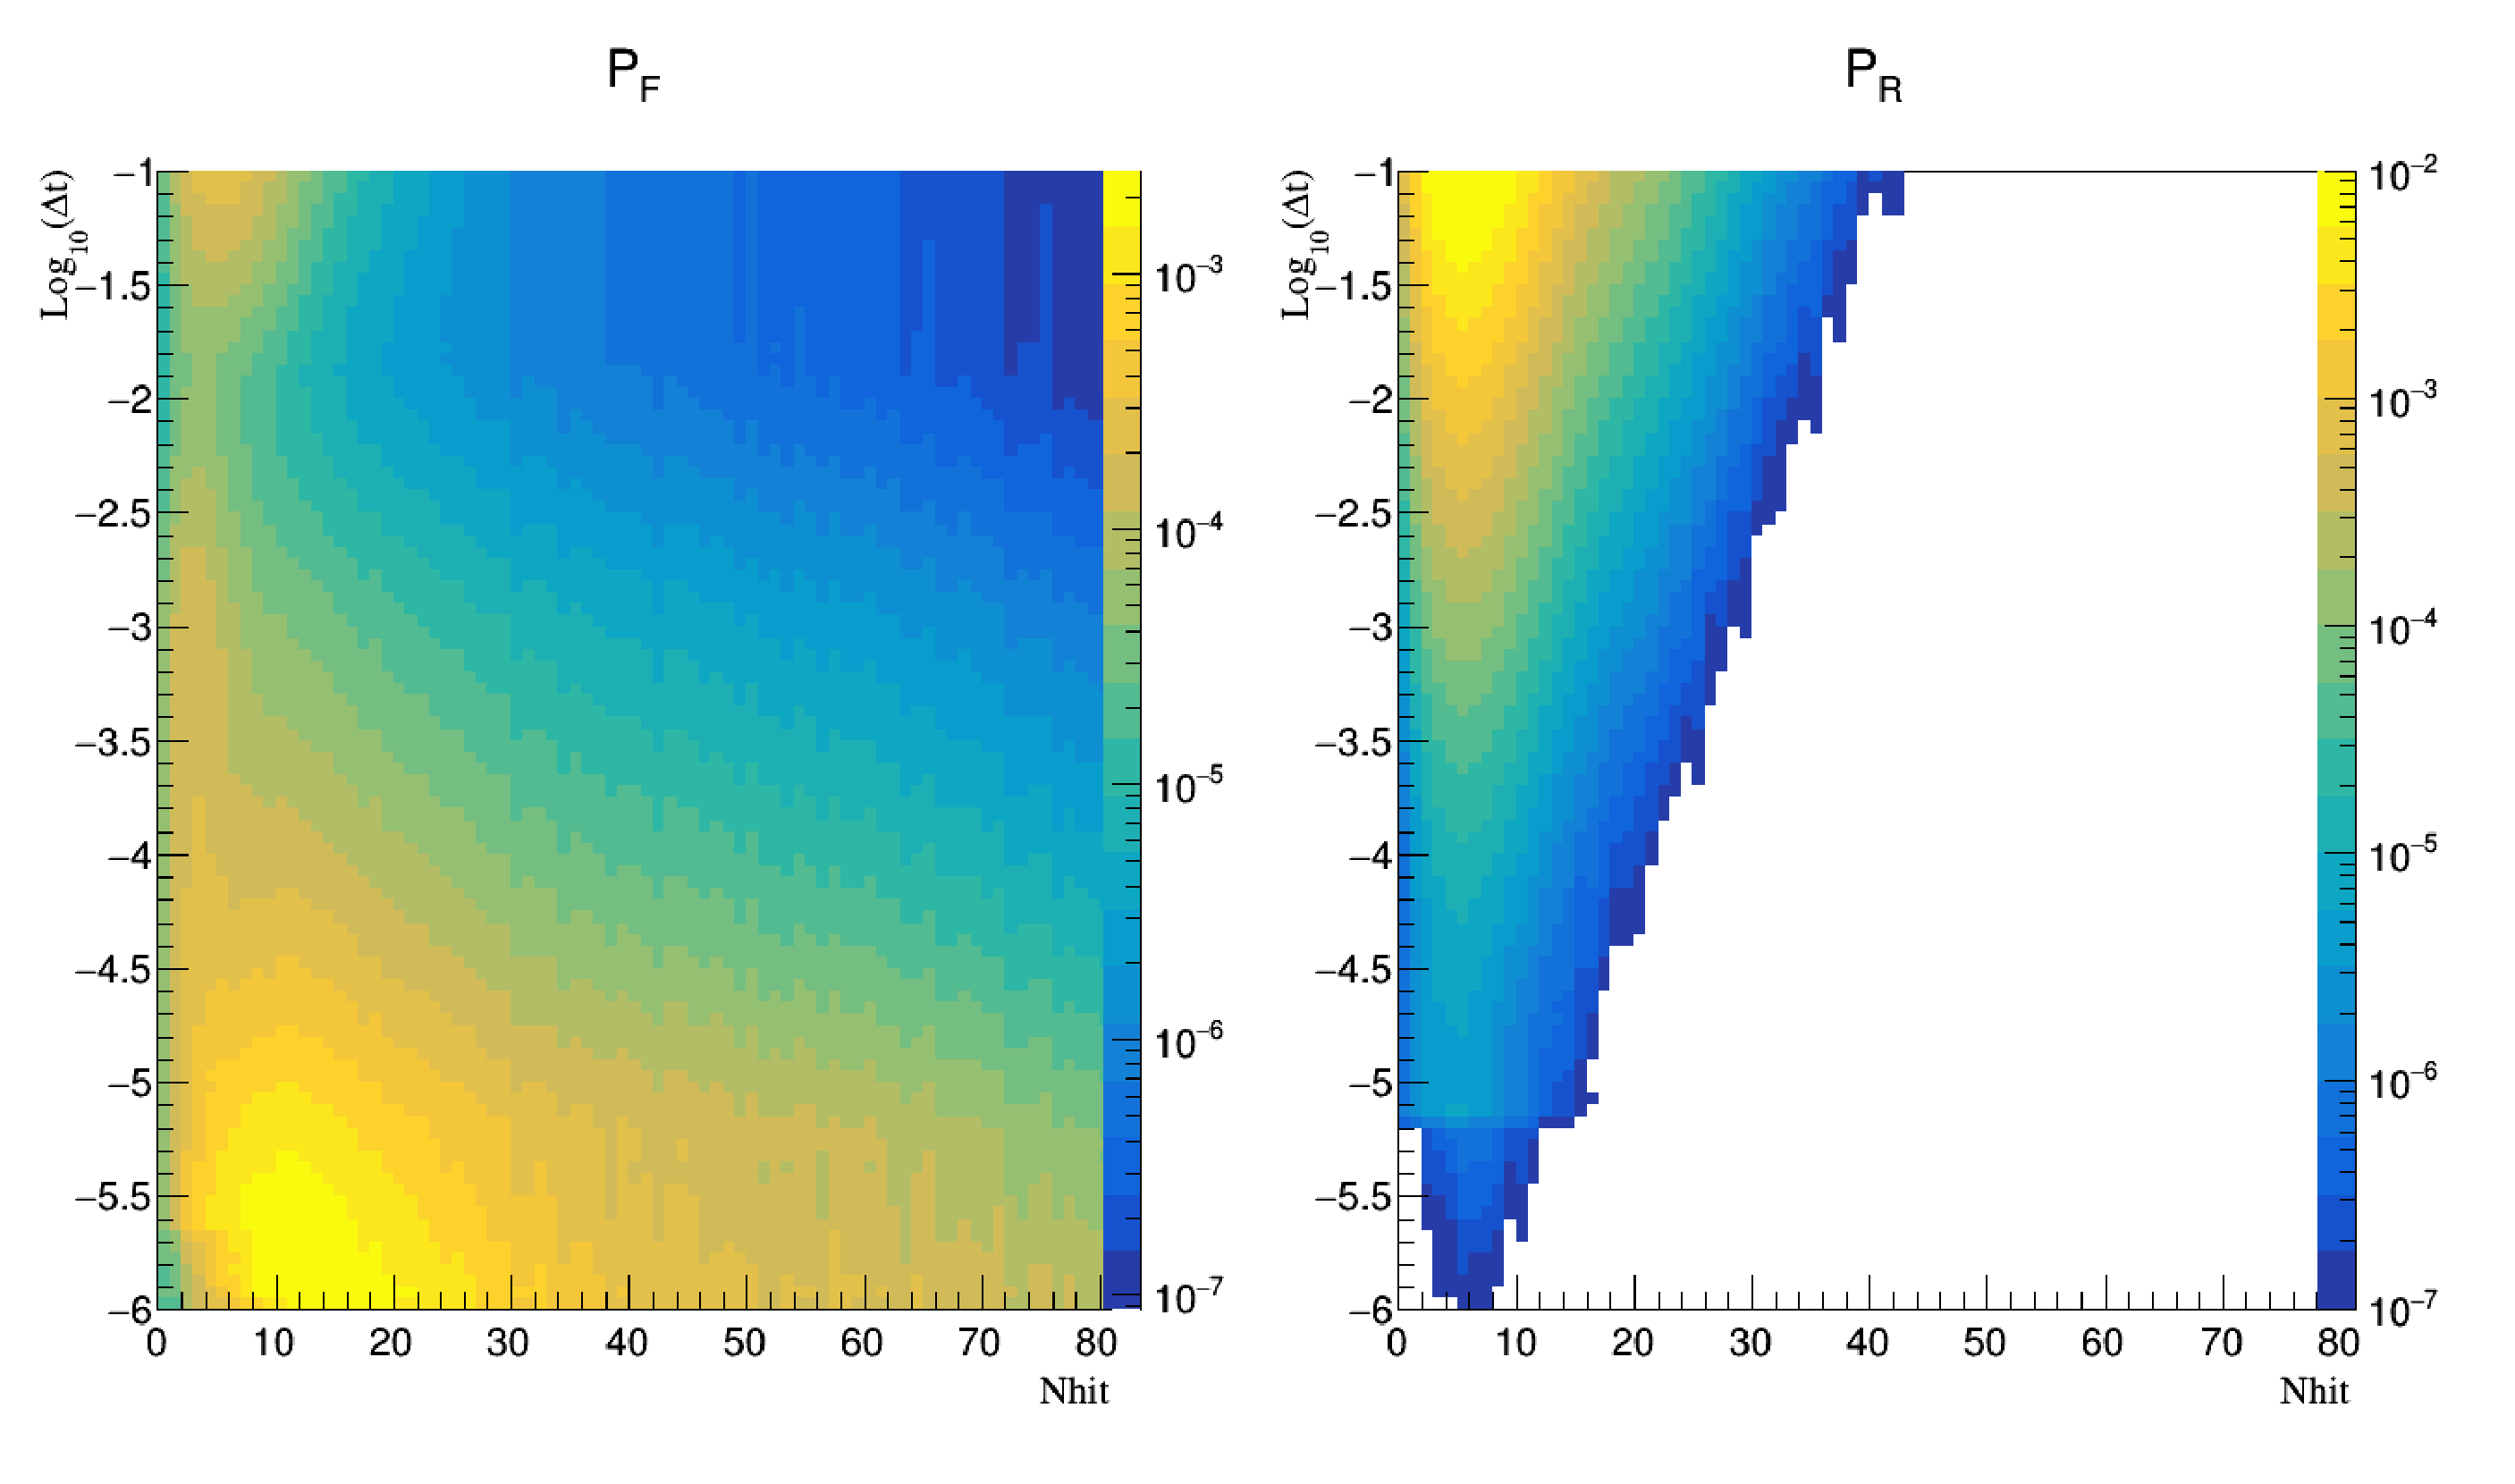
\includegraphics[width=0.74\textwidth]{mmf_bin_volume_normalized}
    \caption[Two-Dimensional Comparison for Missed Muon Follower]{
}
\label{fig:mmf_sac2}
\end{figure}
Figure~\ref{fig:mmf_sac} shows the measured distributions for $P_{F}$ and $P_{R}$
evaluated during the unblinded portion of the dataset;
a number of features exist in the observed distribution for $P_{F}$,
the peak at very short $\Delta t$ comes from re-triggers within the
detector following a high-nhit event.
Figure~\ref{fig:mmf_sac2} shows this comparison in two dimensions, each
bin along the Y-axis is normalized to account for the logarithmic change
in effective bin size.

Since there exists a number of selections from the threshold values of $N_{1}$,
$N_{2}$ and $\delta T$, the threshold value for $N_{1}$ was fixed at the SNO value
of $60$~\citep{neil_thesis}.
This value is motivated by the fact that time correlated events are more
likely to follow highly energetic events or events that can produce cosmogenic
isotopes, and the nhit threshold for these processes is not effected significantly
by the changes from SNO to SNO+.
The threshold value for $N_{2}$ was selected based upon what nhit of event
could possibly serve as a background to the solar or nucleon decay analysis,
a conservative value of $20$ was selected, which corresponds to an electron kinetic energy
of approximately $3$\,MeV.
With the two nhit constraints selected the $\delta t$ window was selected to
be as large as possible without incurring significant signal sacrifice,
the threshold value of $1$\,ms was selected.
From this a sacrifice of $0.01\%$ percent was determined~\citep{dc_document}.

\subsubsection{CAEN Cut}
I developed a new data cleaning cut, called the ``CAEN Cut'', that follows from
the AMB Cut from SNO\@.
The AMB Cut attempted to remove events from flashers the dataset by requiring
that the integral and peak height of the ESUMH trigger sum (as measured by the
AMB) fall below some threshold value.
The CAEN Cut performs a similar function, it calculates the baseline subtracted
integral and peak height of the digitized ESUMH trigger signal and places a cut on those values.

The baseline value of each trace is calculated as the average value of the first
$20$ samples and the $65^{\text{th}}$ to $85^{\text{th}}$ samples.
I chose to use two windows, one before the trigger pulse, one after the trigger pulse, to
correct for any overall slope across the digitized window.
The CAEN window is $104$ samples long, the final 19 samples are not used because they often
include a large noise pulse.
The noise pulse comes from the GT pulse arriving at the front-end and generating electrical noise,
it's typically called ``GT pickup''.
The noise makes the last $\approx20$ samples of the CAEN trace nearly
useless.

The determined baseline is subtracted from the CAEN trace and the integral and maximum
peak height are calculated from the samples between the two baseline windows.
To pass the CAEN Cut the peak and integral must fall between an upper and lower, nhit dependent,
cut cut value.
The cut values are given by
\begin{equation}
    f(n) = C\left(1-\sigma(n)\right) + \sigma(n)\left(mn+b\right)\text{.}
    \label{eqn:cc_threshold}
\end{equation}
Here $\sigma(x)$ indicates a sigmoid function,
\begin{equation}
    \sigma(x) = \frac{1}{1+e^{\frac{-(x-x_{0})}{w}}}
\end{equation}
The cut values are meant to be constant value at lower nhit, and then
linear with nhit above $\approx15$ nhit, the sigmoid allows for a smooth
transition between those two functions; for both the upper and lower threshold
the sigmoid position ($x_{0}$) and width ($w$) are $15$\,nhit and $5$\,nhit respectively.
The constant value at lower nhit is $C$ the slope of the line at higher nhit
is given by $m$ and the value $b$ is required to be
\begin{equation}
    b = \frac{C}{mx_{0}}
\end{equation}
so that there is not discontinuity between the two cut regions.
\begin{table}
    \centering
  \begin{tabular}{c | c c}
      & Constant & Slope  \\
      \hline
      Upper Bound & 658.8 & -6.61\\
      Lower Bound & -707.0 & -15.9\\
    \end{tabular}
    \caption[CAEN Cut Values]{The upper and lower bounds for the CAEN Cut as
    described in Eqn.~\eqref{eqn:cc_threshold}.
    Constant values are in ADC Counts, slope values are ADC Counts per nhit.}
\label{tbl:caen_cut}
\end{table}
The values for these parameters are given in Table~\ref{tbl:caen_cut}.

The reason for the two cut regions is because at lower nhit the signal
peak is smaller than the noise one the ESUMH signal, so the only requirement
is that the peak and integral be consistent with a noise only trigger sum.
At higher nhit the ESUMH signal scales linearly with nhit, each new hit
adds approximately the same amount of height to the trigger pulse.

The cut parameters were determined from two calibration datasets, the first was
tagged $\ce{^{16}N}$
events. The second was a sample of $PULSE\_GT$ triggers taken during normal
running.
The two datasets are used to determine the cut parameters for the two
different cut regions.
The $\ce{^{16}N}$ data was used to determine cut values for the higher nhit
region, the $PULSE\_GT$ data was used for the lower nhit cut values.

\begin{figure}[htbp]
    \centering
    \begin{subfigure}[b]{0.48\textwidth}
        \centering
        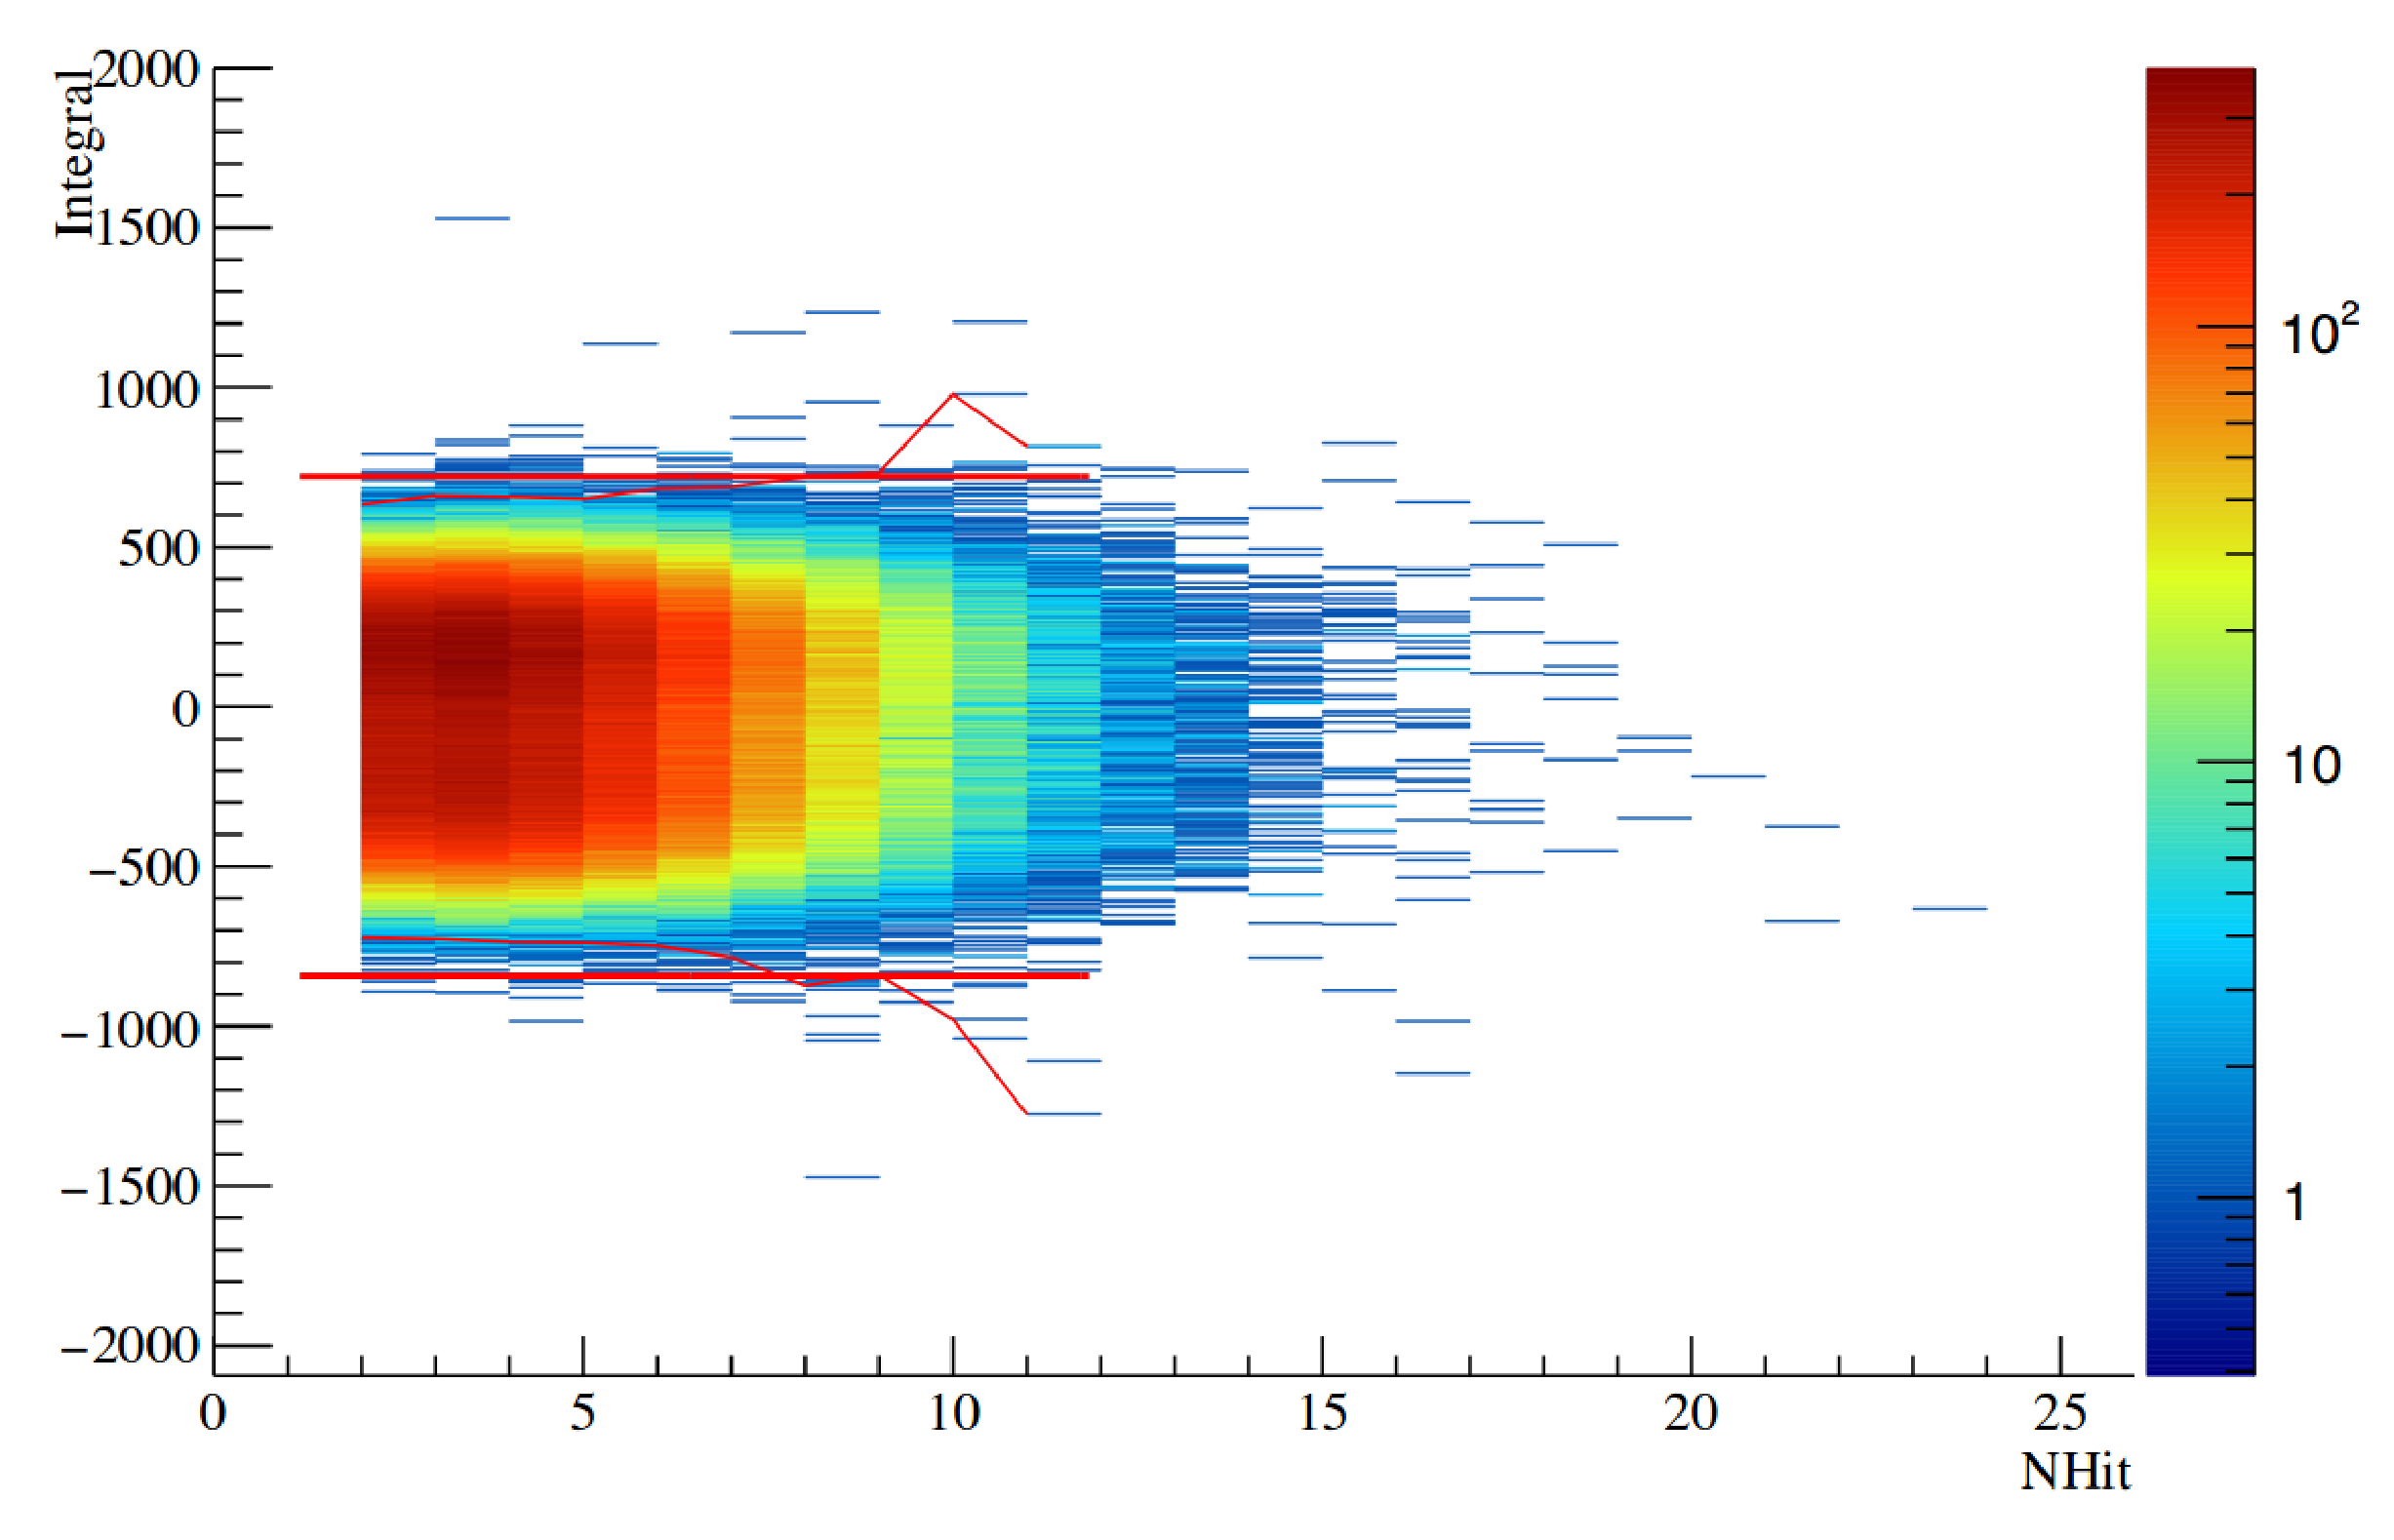
\includegraphics[width=\textwidth]{caen_pgt}
        \caption[]{}
    \end{subfigure}
    \hfill
    \begin{subfigure}[b]{0.48\textwidth}
        \centering
        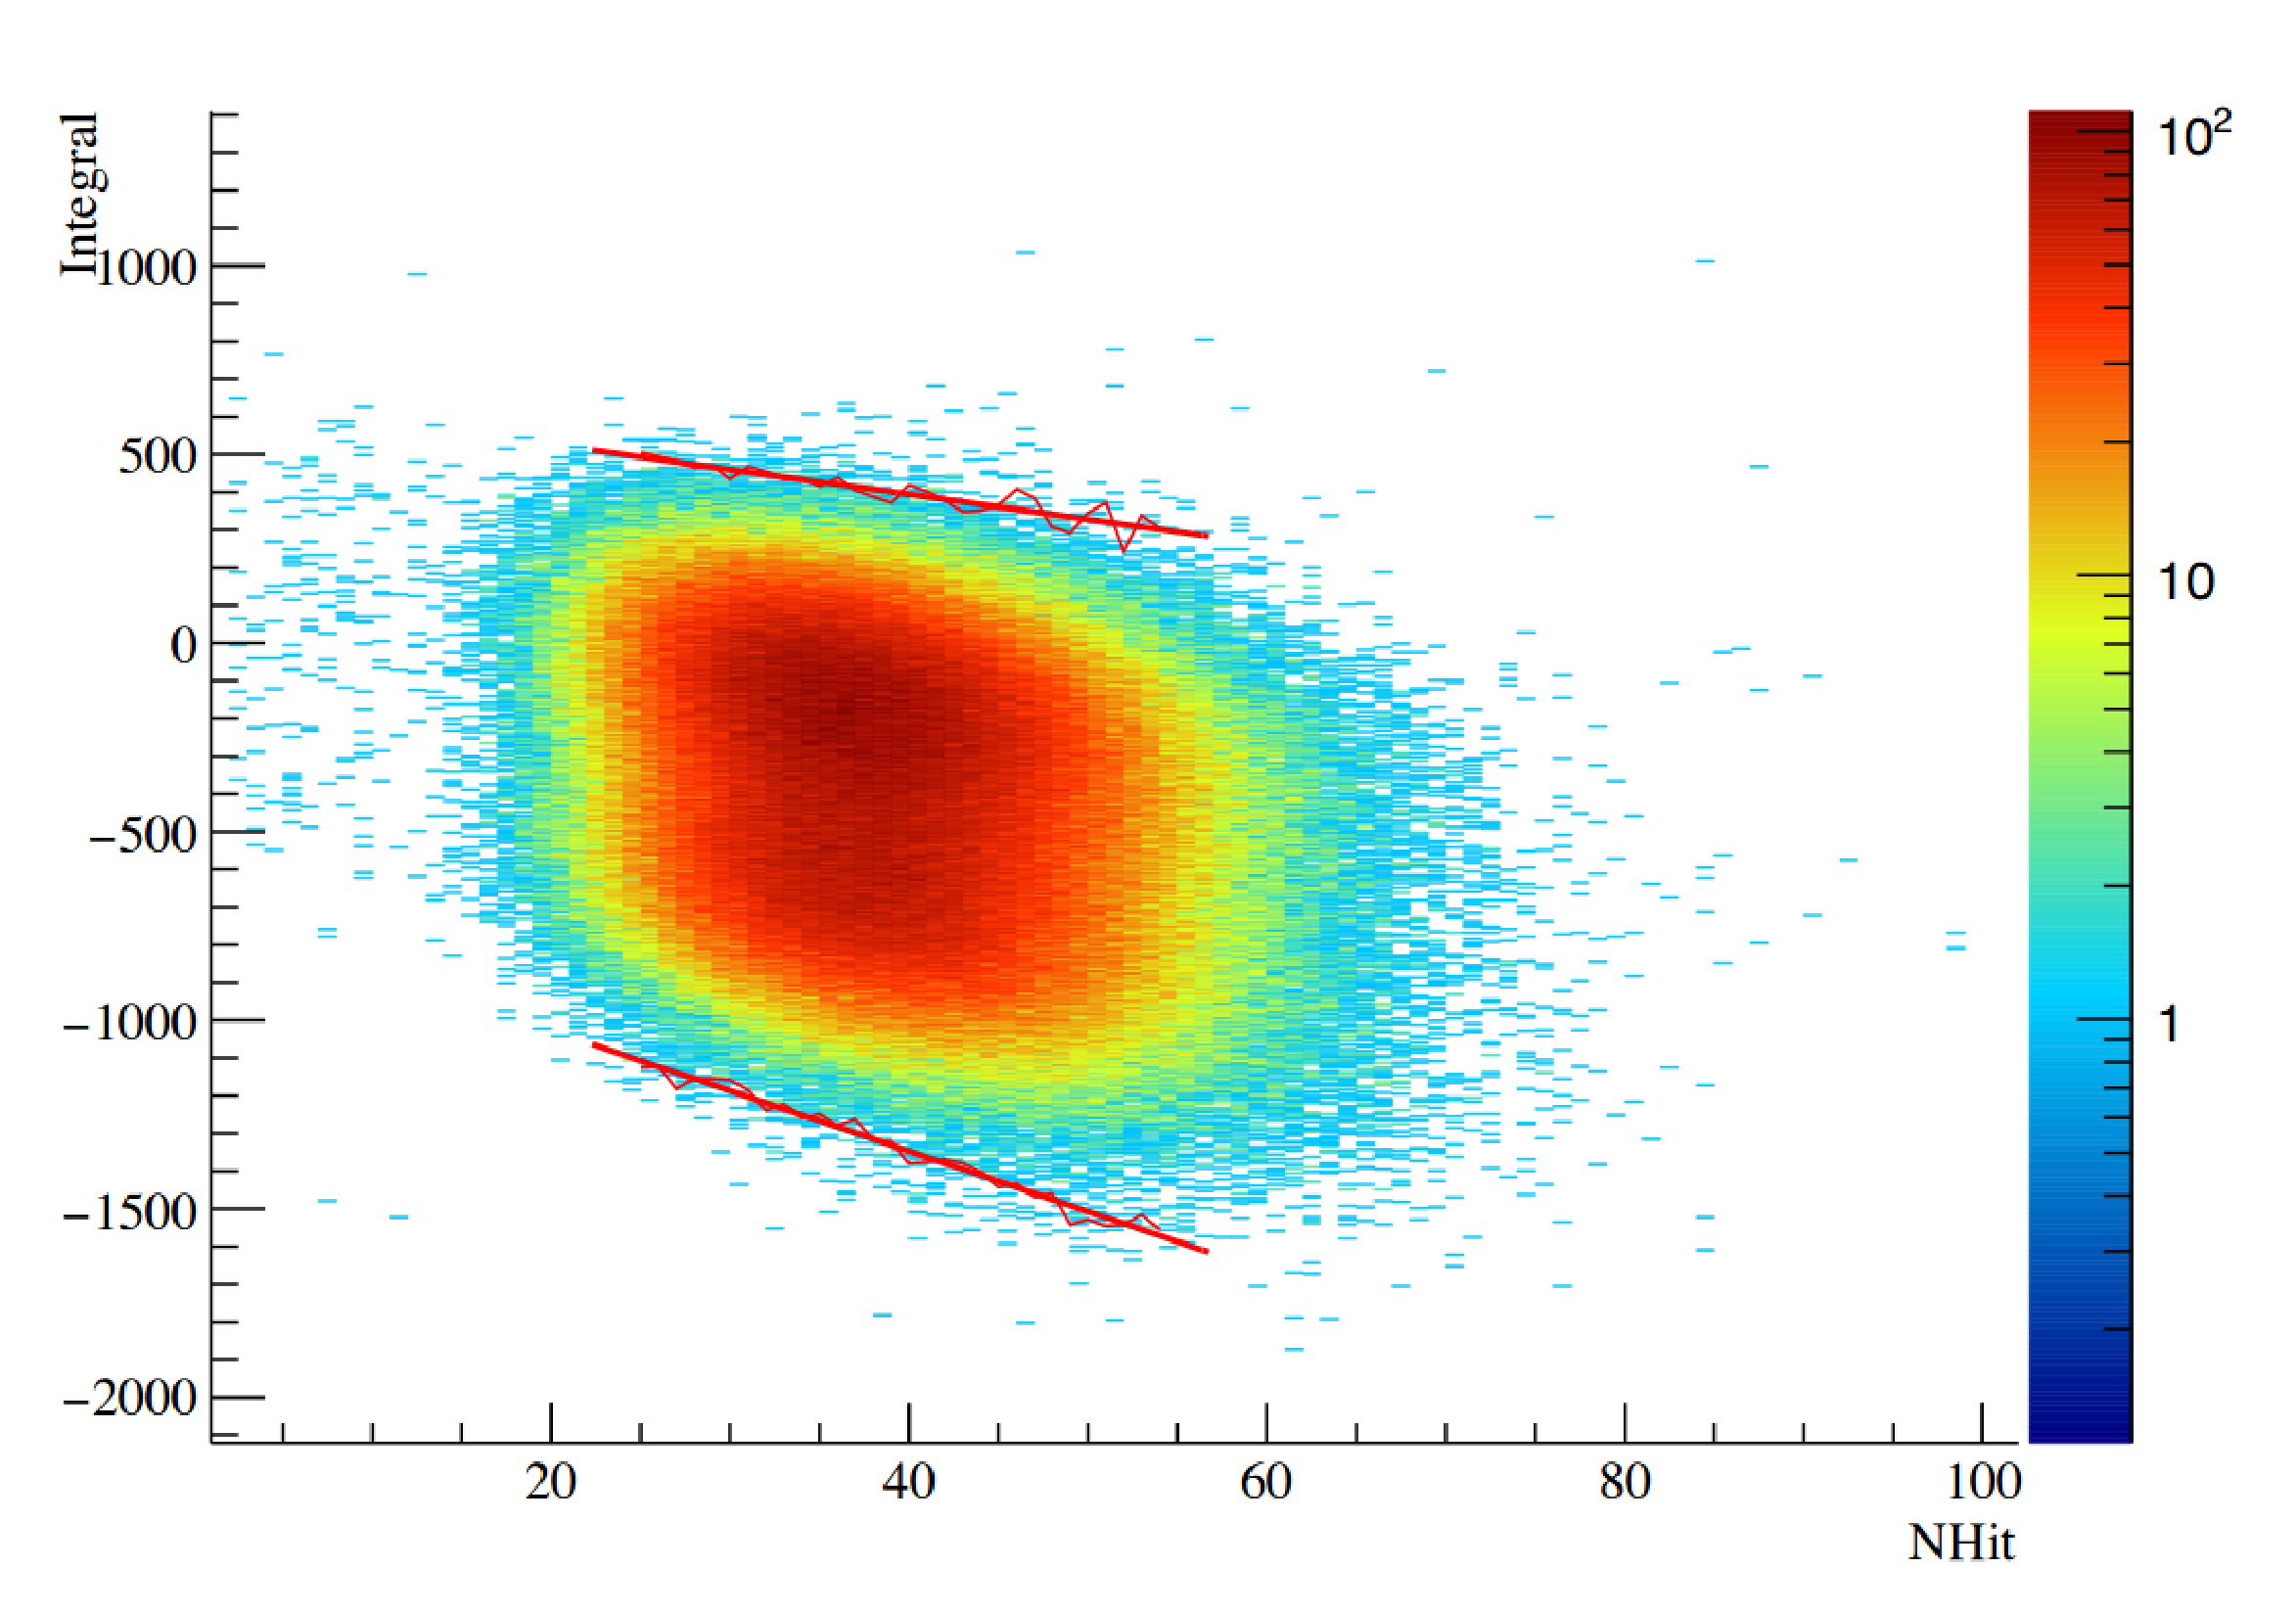
\includegraphics[width=\textwidth]{caen_n16}
        \caption[]{}
    \end{subfigure}

    \begin{subfigure}[b]{0.50\textwidth}
        \centering
        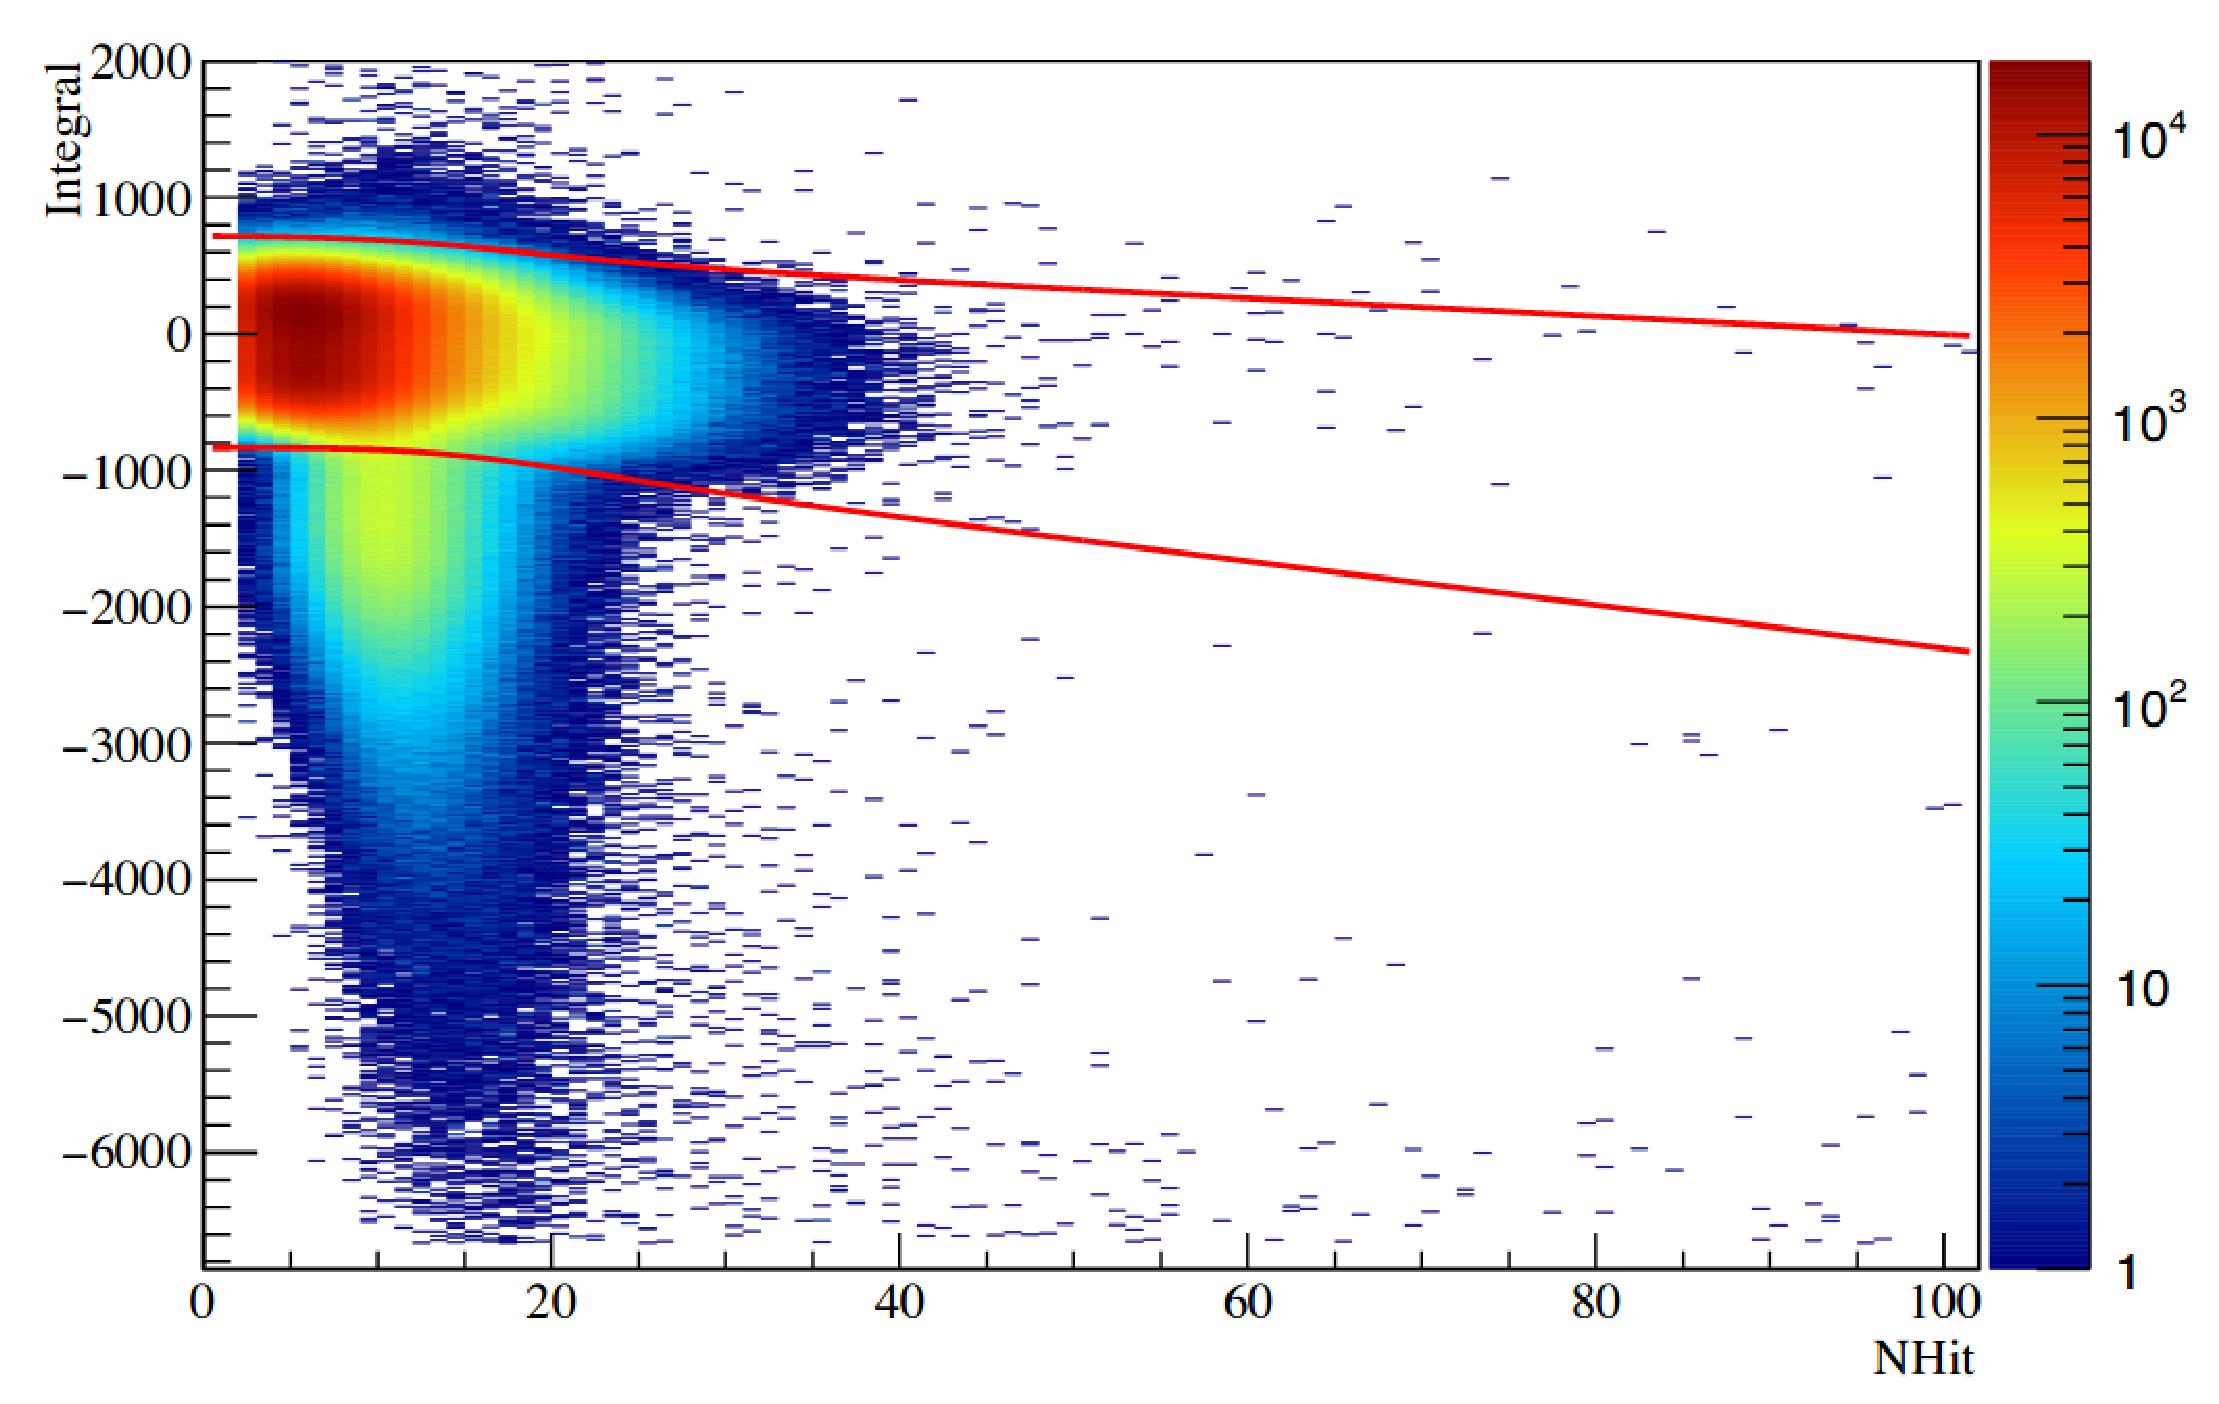
\includegraphics[width=\textwidth]{caen_physics}
        \caption[]{}
    \end{subfigure}
    \caption[]{Distribution of CAEN integral for $PULSE\_GT$ (a), $\ce{^{16}N}$ (b), and
    standard physics triggered (c) events. Integral values are in ADC counts
    and Z-axis values are counts. The thin red lines indicate the 99\% inclusion
    values and the thick red lines indicate the best fit functions.}
    \label{fig:caen_inclusion}
\end{figure}

For both regions the value of the integral or peak height that include
99\% of the events at each nhit is found. Then the parameters of
Eqn.~\ref{eqn:cc_threshold} that best fit those points is determined.
Then Eqn.~\ref{eqn:cc_threshold} with the best fit upper and lower
parameters to include 99\% of the calibration data become the threshold
values for rejecting flasher events.
The 99\% criteria was chosen arbitrarily to ensure that the fraction of
``good'' events rejected by this cut was similar to that of other data
cleaning cuts.
Figure~\ref{fig:caen_inclusion} shows how the ESUMH CAEN trace integral is distributed
in the two calibration datasets and for standard physics data taking.



%TODO move this shit to an appendix
%\subsection{ZeroZero Cut}
%The GTID for the FEC is stored in a ripple counter, it's often the case that
%when the bottom two bits of the counter rollover the event that gets recorded in
%the FEC memory gets corrupted.
%When this happens the builder cannot put the corrupted hits into the event correctly,
%and the hits will effectively be discarded.
%This means that event the detectors effective photon detection efficiency is lower
%for events that have a GTID with $00$ in the bottom two bits.
%Rather than correct for this inefficiecy in reconstruction, events with GTID
%ending in $00$ are discarded. This corresponds to a random pre-scale
%on our by a factor of $\frac{1}{256}$.
%\subsection{Crate Isotropy Cut}
%The Crate Isotropy Cut is designed to remove events that are isolated
%in one or a few electronics crates.
%Events originating from light within the detector are unlikely to have any
%preference in electronics space.
%However hits caused by electrical noise that was created near the electronics
%can show a very distinct preference for one crate.
%The criteria for this cut is that fraction of hits in any single
%is greater that $70\%$ and that the fractions of hits within
%that crate are either $80\%$ within adjacent FECs or $70\%$ within
%adjacent channels.
%%\subsection{Flasher Geometry Cut}
%%\subsection{ITC Timespread Cut}

\section{Analysis Cuts}
\label{sec:analysis_cuts}
The dataset of events passing all data cleaning cuts is further reduced by
requiring all events pass cuts on reconstructed quantities.
The cuts are designed to minimize the number of events in the dataset from
non-solar interactions.

Necessarily, the first of these cuts is the requirement that the reconstruction
fits produce to a valid position, time and energy.
The reconstruction algorithms can fail to converge if an event occurs in an
optically complicated region of the detector, \textit{e.g.} near the detector
neck. The fitting algorithms rely on the assumption that the majority of
the produced light will travel directly from the event vertex to PMT array.
For events in optically complicated regions this assumption is not a good one.
These regions modelled in simulation, so the Monte Carlo simulation estimate of
the efficiency of reconstruction to produce valid fits for solar neutrino events
is used.

A cut, called the ``trigger efficiency'' cut,  is placed on the number of
in-time nhits in each event.
This cut ensures the dataset occupies a region where the detector trigger
efficiency is well understood and near 100\%.
This cut ensures the analysis is minimally effected by uncertainties
associated with the detector's trigger.
As mentioned in Sec.~\ref{sec:dataset}, the detector trigger threshold were adjusted
part way through data-taking. The in-time nhit cut was adjusted to
account for this.
For the first trigger period all events were required to have an in-time
Nhit greater than or equal to $23$; for the second trigger period this
threshold was reduced to $10$.
This cut is similar to an energy cut because nhit is the best energy estimator
for an event. But, as discussed below, events passing the analysis energy cut
are very unlikely to fail the trigger efficiency cut.

The next analysis cut is a fiducial volume (FV) cut that requires all events
be within $5.3$\,m of the center of the detector.
This cut is designed to reduce the background from radioactive decays within
the AV or from the water outside the AV\@.
During the hot-spot time period the FV cut was modified to require any events in the
top half of the detector ($z > 0$) fall within a radius of $4.2$\,m,
events in the bottom half of the detector were still subject to the standard
$5.3$\,m FV cut.
The more restrictive cut was in place for 13\% of the dataset livetime.
%Figure {XXX} shows the expected distribution of background events from AV and external water backgrounds compared to the distribution for solar neutrino events.

The time residual, defined in equation~\ref{eqn:tres} for a PMT hit is an extremely
useful quantity because in general light that travels directly from an
interaction will have a very small time residual.
Light that is produced by another source, or reflects off of a detector component
between production and detection will have a larger time residual.


The fraction of hits that satisfy
\begin{equation}
    -2.5 < t_{res} < 5
\end{equation}
is known as the ``In-time ratio'' (ITR).
%The expected distribution in ITR for electrons is shown in figure XXX.

The quantity $\beta_{14}$ is used to quantify how isotropic the hits
in an event is. It is defined as
\begin{equation}
    \beta_{14} = \beta_{1} + 4\beta_{4}
\end{equation}
where
\begin{equation}
\beta_{\ell} = \frac{2}{N(N-1)}\sum_{i=1}^{N-1}\sum_{j=i+1}^{N}P_{\ell}(\cos\theta_{ij})\text{.}
\end{equation}
$P_{\ell}$ is the $\ell^{\text{th}}$ Legendre Polynomial and
$\theta_{ij}$ is the angle subtended by the vectors pointing
from the reconstructed position of the event to the $i^{\text{th}}$ and
$j^{\text{th}}$ hit PMT\@.

Cuts are placed on the ITR and $\beta_{14}$ value for each event.
These cuts aim to remove events
that have an ITR or $\beta_{14}$ 
that is inconsistent with the event originating from Cherenkov light produced
by a solar neutrino event.
The ITR of events is required to be greater than $55$\% and the $\beta_{14}$
value must between $-0.12$ and $0.95$.
These cuts are similar in purpose to the data cleaning cuts, as they attempt to
remove events that are produced by sources other than Cherenkov light within
the detector.

The final analysis cut is on the reconstructed kinetic energy of each event.
The energy region for this analysis is $5.0 < T_{\mathrm{e}} < 15.0$\, MeV.
This region is chosen to minimize contamination from atmospheric neutrino
interactions, and radioactive decays within the detector.
Additionally, the only solar neutrino flux that is significant across this energy range
are the neutrinos from the $\ce{^{8}B}$ solar reaction.
Neutrinos from the $hep$ interaction also fall within the same energy range,
however their flux is expected to be much lower than that of the $\ce{^{8}B}$
neutrino flux that their presence can be largely neglected.

In principle the lower energy threshold could be lowered or removed to
increase the efficiency for solar neutrino events, however,
the rate of backgrounds from radioactive decays increases rapidly at lower
energies. So no additional sensitivity to the solar neutrino interaction
rate would be gained with a lower energy threshold.
The $5$\,MeV threshold was chosen as the lowest energy from which a solar
signal could still be resolved.
%A summary of all cuts and their criteria, where applicable, is given in Table~\ref{tbl:event_selection}.

%\begin{table}
%    \centering
%  \begin{tabular}{c  c}
%      Energy & FV & Data Cleaning & ITR & $\Beta_{14}\\
%    \end{tabular}
%    \caption{Cuts}
%\label{tbl:event_selection}
%\end{table}


\chapter{Analysis}
\label{sec:analysis}
\section{Signal Extraction}
Once an MC simulated dataset and a detector dataset are selected, the analysis
of those events is performed.
The first steps of the analysis is to bin all events
in a two-dimensional histogram of reconstructed energy and $\cos\theta_{\mathrm{sun}}$.
Events are distributed across $N_{\theta}$ equal width bins in $\cos\theta_{\mathrm{sun}}$ from
\numrange{-1}{1} and
$N_{E}$ bins in energy from \numrange{5.0}{15.0}\,MeV.
For this analysis $N_{\theta}$ is 40 and $N_{E}$ is 6.
From \numrange{5.0}{10.0}\,MeV $5$ bins of width $1$\,MeV are used and
a single bin from \numrange{10.0}{15.0}\,MeV is used.
Simulated and detected events are placed into separate histograms.

Simulated $\nu_{e}$ and $\nu_{\mu}$ events are histogrammed separately,
but given different weights in their respective histogram according to the expected survival probability
for each event.
The weight for a $\nu_{e}$ event with neutrino energy $E_{\nu}$ is given by,
\begin{equation}
    w_{\mathrm{e}} = P_{\mathrm{ee}}(E_{\nu})\text{,}
\end{equation}
and the weight for a $\nu_{\mu}$ event is given by,
\begin{equation}
    w_{\mathrm{\mu}}= P_{\mathrm{e\mu}} = 1 - P_{\mathrm{ee}}(E_{\nu})\text{.}
\end{equation}

As mentioned in Sec~\ref{sec:simulation} the effective flux of the solar
simulations are much larger to than the expected flux of the detected dataset;
this scaled flux is the same as if the simulated dataset had a much higher livetime
but a standard flux value.
So the simulated histograms are
scaled to by $\frac{t_{live}}{t_{sim}}$ to make the effective simulated
livetime match the livetime of the detector dataset.
An additional scaling is done to the simulated histograms to account
for the data cleaning, this is needed because data cleaning
is not applied to simulated events.
The data cleaning rejection rate was determined to be $1.2\%$, so the
simulated histograms are scaled by a factor of $0.988$.

Once these scales are applied the $\nu_{e}$ and $\nu_{\mu}$ histograms
respectively  represent the expected distribution and event rate for the charged current
and neutral current interactions in the dataset for the nominal $\ce{^{8}B}$
solar neutrino flux used in simulation.
The $\nu_{e}$ and $\nu_{\mu}$ histograms are then combined by
simply adding their bin contents together to get the expected
mixed flavor elastic scattering interaction rate as a function
of $T_{\mathrm{e}}$ and $\cos\theta_{\mathrm{sun}}$.
Applying additional scaling to this combined histogram is done to represent
a hypothesized scaling to the overall solar neutrino flux.
So the rate of solar neutrino events is given by
\begin{equation}
    R_{\nu}(\cos\theta_{\mathrm{sun}}, T_{\mathrm{e}}) =
    S\phi(R)
    \label{eqn:solar_rate}
\end{equation}

Equation~\eqref{eqn:solar_rate} is modified slightly to include a parameter
related to the detector angular resolution, $\delta_{\theta}$,
\begin{equation}
R_{\nu}(\cos\theta_{\mathrm{sun}}, T_{\mathrm{e}}) \rightarrow
    R_{\nu}(\cos\theta_{\mathrm{sun}}, T_{\mathrm{e}}, \delta_{\theta})\text{.}
\end{equation}
This modification is discussed more in Sec~\ref{sec:angular_systematics}.

No simulation or measurements were done for the expected backgrounds for this analysis,
so a simple background model is adopted.
It is assumed that the direction of any background event will be uncorrelated
with the position of the sun, this is what makes $\cos\theta_{\mathrm{sun}}$ such a
useful variable in this analysis.
The distribution of background events is given by
\begin{equation}
    R_{\mathrm{B}}(\cos\theta_{\mathrm{sun}}, T_{\mathrm{e}}) =
    R_{\mathrm{B}}(T_{\mathrm{e}}) = \frac{1}{N_\theta}n_{\mathrm{B}}(T_{\mathrm{e}})
\end{equation}
Where $n_{\mathrm{b}}(T_{\mathrm{e}})$ is number of background events in the
histogram energy bins corresponding to the energy $T_{\mathrm{e}}$.
The number of background events in each energy bin are not known \textit{a~priori}
and are treated as a nuisance parameter in the remainder of the analysis.

The total expected events in each bin can be expressed by
\begin{equation}
    R(\cos\theta_{\mathrm{sun}}\text{, }T_{\mathrm{e}}) =
    R_{\mathrm{B}}(T_{\mathrm{e}}) + R_{\nu}(\cos\theta_{\mathrm{sun}}\text{, }T_{\mathrm{e}}\text{, }\delta_{\theta})\text{.}
    \label{eqn:event_rate}
\end{equation}

The unknown parameters of this rate are the 6 background rates and the solar
rate and $\delta_{\theta}$.
A fit to data is performed for equation~\eqref{eqn:event_rate} to extract
those parameters.
Goodness-of-fit is evaluated using a likelihood given by
\begin{align}
    \mathcal{L}(S&, \bold{B}, \delta_{\theta} | \bold{n}, \mu_{\theta}, \sigma_{\theta}) = \nonumber\\
    &\mathcal{N}(\delta_{\theta}, \mu_{\theta}, \sigma_\theta)
    \prod_{j=0}^{N_E}\prod^{N_{\theta}}_{i=0} \text{Pois}\left(n_{ij},\, B_{j} + S\,p_{ij}(\delta_{\theta})\right)\text{.}
    \label{eq:ll}
\end{align}
The parameters $\mu_{\theta}$ and $\sigma_{\theta}$ are respectively the best
fit and the constraint on $\delta_{\theta}$ from the $\ce{^{16}N}$ source
analysis.
$\text{Pois}\left(k, \lambda \right)$ is the value of the Poisson distribution
at the value $k$ for a rate parameter $\lambda$.

Equation~\eqref{eq:ll} can be modified to fit for the solar rate in individual
energy bins, rather than constraining the solar rate to be the same across
all energy bins. This is done by replacing the product over energy bins,
$\prod_{j=0}^{N_E}$, with the selection of $j=0\text{, }1\text{, }$\textit{etc.}
Fitting for a solar rate in each bin allows for a spectral measurement of the
solar neutrino flux, as opposed to an integrated flux measurement.

\section{Systematics}
Systematics associated with event reconstruction, livetime, mixing parameters,
and trigger efficiency are considered for this analysis.
The event reconstruction systematics are uncertainties on the energy reconstruction
scale and resolution, position reconstruction resolution and scale, and the
resolution of the direction reconstruction.
The uncertainties on each of these values and how they were determined is
discussed in Sec~\ref{sec:calib}.

Each systematics is treated in the same, or a similar, way, to propagate
their effect to the flux result.
The systematics are propagated through the analysis by modifying the
relevant quantities on reconstructed monte-carlo events according to the
one-$\sigma$ uncertainty.
The PDFs that result from the modified events are used in the analysis to extract
a flux result.
The difference between the systematically adjusted flux result and the standard
result is taken to be the one-$\sigma$ systematic uncertainty.
How each variable is modified, and any deviations from this process of
propagating systematics is detailed below.
All systematics are treated as uncorrelated, that is variables are modified according to
only one systematic at a time.

\subsection{Energy Resolution}
The energy resolution uncertainty is determined primarily from the $\ce{16}N$ analysis.
The systematic uncertainty on the energy resolution was determined to be $\delta_{\sigma} = +1.8\%, -1.6\%$. %TODO
To create the energy resolution systematic's modified PDFs the reconstructed
energy of the MC simulated events is mapped to a normalized Gaussian distribution with a
mean value of the event's energy and a
variance given by
\begin{equation}
  \sigma^{2} = \sigma_{E}^{2}\left(\left(1 + \delta_{\sigma}\right)^2 - 1\right)\text{.}
  \label{eqn:systmatic_esmear}
\end{equation}
This process of mapping a single energy value to a Gaussian distribution is referred to as ``smearing''.
Here $\sigma_{E}$ is given by $\sqrt{E}$ to match the functional form used in the fit for the systematics,
Eqn~\ref{XXX}.
The idea behind this smearing is to compensate for the possibility that our monte-carlo simulation could have
a systematically smaller energy resolution than occurs in real data.
So by applying a smearing the monte-carlo energy resolution is artificially deteriorated, and the uncertainty
on the resolution is accounted for.
A similar process does not exists to account for the possibility that the monte-carlo simulation has a poorer
energy resolution than data taken from the real detector; there's no way to ``un-smear'' the reconstructed MC
event energy.
So, to account the effect of an over-estimated energy resolution the error on the result is assumed to be symmetric.
As a penalty for this assumption the larger uncertainty between the positive and negative uncertainty on the
energy resolution is used.

If the smeared event passes all cuts then each energy binned

\subsection{Energy Scale}
Systematically varied PDFs for the energy scale PDF is generated by simply modifying the reconstructed
kinetic energy of each event according to
\begin{equation}
  T^{\prime}_{e} = (1+\delta_{E})T_{e}\text{.}
\end{equation}
At all points in the analysis afterwards $T^{\prime}_{e}$ is used instead of $T_{e}$.

\subsection{Fiducial Volume}
Uncertainty on the fiducial volume comes primarily from systematics associated
with the position reconstruction.
If the position reconstruction is more likely to pull an event towards the
middle of the detector
in MC simulation than in data, it will result in an over prediction of the
number of events that will pass the FV cut.
This possibility is accounted for by shifting the reconstructed position of
simulated events according to the uncertainty, the fiducial volume cut is
applied to those shifted positions.  Shifting the events results in modified
PDFs, those PDFs are used in the fit for the solar event rate, the difference
between the best fit value extracted with the modified PDFs and the best fit
value from the standard PDFs is taken to be the systematic uncertainty.
\subsection{Angular Resolution}
The angular resolution uncertainty is treated differently from other
uncertainties because the distribution of events in $\cos\theta_{sun}$ is
directly related to the direction resolution.  To minimize the impact the
angular resolution has on the result it is used as one of the parameters in the
fit to the $\cos\theta_{sun}$ solar neutrino distribution, and constrained by
the results of the $\ce{^{16}N}$ analysis.

The angular resolution systematic is applied using the formula given in
~\ref{sec:angular_syst},
\begin{equation}
    \cos\theta^{\prime} = 1 + (\cos\theta - 1)(1+\delta_{\theta})\text{.}
    \label{eqn:angular_syst_map}
\end{equation}
Where $\theta$ is the angle between the true event direction and the reconstructed
event direction, and $delta$ is the angular resolution systematic uncertainty.
Using~\eqref{eqn:angular_syst_map} has the unfortunate downside producing
unphysical values for $\cos\theta^{\prime}$ for values of $\cos\theta$ near
$-1$. For values of $\cos\theta^{\prime}$ below $-1$ the value is instead replaced
with a random value drawn from a uniform distribution $\left[-1\text{, }1\right]1$.
The logic behind this choice is that when an event reconstructs with a direction
that's nearly $180^{\circ}$ from the correct value, then the reconstruction
has likely failed to such a degree that the reconstructed values are uncorrelated
with the true values, and so drawing from a uniform random distribution preserves
that uncorrleated nature without adding any additional bias.

Once the systematically varied value for $\cos\theta$ is determined, the new angle
needs to be transformed into a corresponding direction vector for the particle.
To do this first a vector that is normal to the plane spanned by the reconstructed
and true direction vector is found by taking the cross-product between those vectors,
\begin{equation}
    \vec{v}_{\mathrm{norm}} = \vec{d}_{\mathrm{true}} \cross \vec{d}_{\mathrm{recon}}\text{.}
\end{equation}
Then $\vec{d}_{\mathrm{recon}}$ is rotated around $\vec{v}_{\mathrm{norm}}$
such that the rotated vector $\vec{d}^{\prime}_{\mathrm{recon}}$ now has an angle
of $\theta^{\prime}$.
The direction $\vec{d}^{\prime}_{\mathrm{recon}}$ is then used in the
analysis to generate event distrubtions in $\cos\theta_{sun}$.

Following this procedure PDFs for $\cos\theta_{sun}$ are generated for many differnt
values of $\delta_{\theta}$, producing $P(\cos\theta_{sun}, \delta_{\theta})$.
The constraint on $\delta_{\theta}$ produced by the $\ce{^{16}N}$ analysis
are included in this two-dimension PDF\@.
$P(\cos\theta_{sun}, \delta_{\theta})$ is used in the remaineder of the analysis
treating $\delta_{\theta}$ as a nuisance parameter.

\subsection{Mixing Parameters}
The central values and uncertainties of the neutrino mixing parameters, $\Delta
m^{2}_{21}$, $\theta_{12}$ and $\theta_{13}$ is taken from Ref.~\citep{pdg_globalfit}.
\begin{table}
    \centering
    \begin{tabular}{c c c}
        Parameter & Value & Uncertainty\\
        $\Delta m^{2}_{21}$ & $7.37\times10^{-5} \mathrm{MeV}/\mathrm{c}^{2}$ & +0.17, -0.16\\
        $\theta_{12}$ & $33.02^{\circ}$ & 0.537, -0.455 \\
        $\theta_{13}$ & $8.41^{\circ}$ & -- \\
        $\Delta m_{31}$ & $2.5e-3\times10^-3\mathrm{MeV}/\mathrm{c}^{2}$ & -- \\
    \end{tabular}
    \caption{A summary of the mixing parameters and their uncertainties as used in 
    propagation of systematic uncertainties. Values from from Ref~\citep{pdg_globalfit}.}
\label{tbl:mixing_values}
\end{table}
The values and uncertainties for the mixing parameters
are summarized in Table~\ref{tbl:mixing_values}.
A survival probability curve is generated for each of the mixing parameters
shifted by their positive and negative one-sigma uncertainty.
These systematically adjusted PDFs are used in the analysis replacing the
standard survial probability curve to propagate the uncertainties to the
flux result.
\subsection{Trigger Efficiency}
The uncertainty on the trigger efficiecy is described in Sec~\ref{sec:trigeff}.
PDFs for $\cos\theta_{sun}$ are generated using the more pessimistic
trigger efficiecy curves measured by the laserball and TELLIE\@.
Simulated events that have an in-time nhit that is predicted by the nhit-monitor
to be 100\% efficient are de-weighted to match the laserball/TELLIE efficiecy
measurement..
The PDFs that result from the de-weighted events are used as the systematically
adjusted PDFs to account propagate the trigger efficiecy uncertainty to the
flux result.
\subsection{Livetime}
Uncertainty on the livetime comes primarily from orphaned events in the detector.
Orphaned detector events are disucssed in~Sec.~\ref{TODOXXX}.
When an orphaned event ocurrs all information about that event is lost including
the time it ocurred and\ldots%TODO! Find documentation from Aobo.


\section{Results}
Figure~\ref{fig:costheta} shows the distribution of events in $\cos\theta_\text{{sun}}$
for events over the entire energy range of $5$ to $15$\,MeV and the fit to that distribution.\
The fit gives a solar event rate of \InteractionRate\
 and background rate of \BackgroundRate.\
Performing a similar fit in each individual energy bin yielded a best fit solar flux
as a function of energy.\
The fits were combined, in accordance with Eq.~\ref{eq:ll}, yielding an overall best fit flux of
\begin{equation*}
    \Phi_{ES}= 2.53^{+0.31}_{-0.28}\text{(stat.)}^{+0.13}_{-0.10}\text{(syst.)}\times10^6\,\text{cm}^{-2}\text{s}^{-1}\text{.}
\end{equation*}
This value assumes the neutrino flux consists purely of electron flavor neutrinos.\
The result agrees with the elastic scattering flux published by Super-K,
$\Phi_{ES}$=\fluxunits{\SuperKRate}~\cite{superk4}, combining statistical and
systematic errors.\

\figuremacro{residual_plot.pdf}{0.5}{spectrum}{
    (Top) The extracted solar neutrino elastic scattering event rate as a
    function of reconstructed electron kinetic energy $T_{e}$.\
    (Bottom) The same, as a fraction of the expected rate.\
    The red and blue lines show the MC simulation predicted spectrum normalized
    to the best fit flux and the SNO flux measurement~\cite{sno_combined}, respectively.\
    The uncertainty on the SNO result includes reported uncertainty combined with
    mixing parameter uncertainties.\
    The black points are the results of the fits to the $\cos\theta_\text{{sun}}$
    distribution in each energy bin,
    with error bars indicating the combined statistical and systematic
    uncertainty, including energy-correlated uncertainty.\
    A horizontal dash is placed on each error bar indicating the statistics
    only uncertainty; for all points the statistical error is dominant and the systematic
    error bar is not visible above the dash.}

\begin{table}
\begin{center}
\begin{tabular}{l c}
\hline
\hline
Systematic & Effect \\
\hline
Energy Scale & 3.9\% \\
Fiducial Volume & 2.8\% \\
Angular Resolution & 1.7\% \\
Mixing Parameters & 1.4\% \\
Energy Resolution & 0.4\% \\
\hline
Total & 5.0\%\\
\hline
\hline
\end{tabular}
\caption{Effect of each systematic uncertainty on the extracted solar neutrino
         flux. Systematic uncertainties with negligible effects
         are not shown. For asymmetric uncertainties, the larger is shown.}
\label{table:systematics}
\end{center}
\end{table}

Including the effects of solar neutrino oscillations, using the neutrino mixing
parameters given in Ref.~\cite{pdg2016} and the solar production and electron
density distributions given in Ref.~\cite{bs05op} gave a best fit solar flux
of
\begin{equation*}
    \Phi_{\ce{^{8}B}}= 5.95^{+0.75}_{-0.71}\text{(stat.)}^{+0.28}_{-0.30}\text{(syst.)}\times10^{6}\text{cm}^{-2}\text{s}^{-1}\text{.}
\end{equation*}
This result is consistent with the \beight flux as measured by the SNO experiment,
$\Phi_{\ce{^{8}B}}$=\fluxunits{\SNOFlux}~\cite{sno_combined}, combining statistical
and systematic uncertainties.\
Figure~\ref{spectrum} shows the best fit solar neutrino \beight event rate in each
energy bin along with the predicted energy spectrum scaled to the best fit
flux, and scaled to the flux measured by SNO. Each statistical error bar on the
measured rate is affected by both the solar neutrino and background rates in that
energy bin.\
Table~\ref{table:systematics} details how each systematic uncertainty affects this result.\

\begin{figure}[htbp]
    \centering
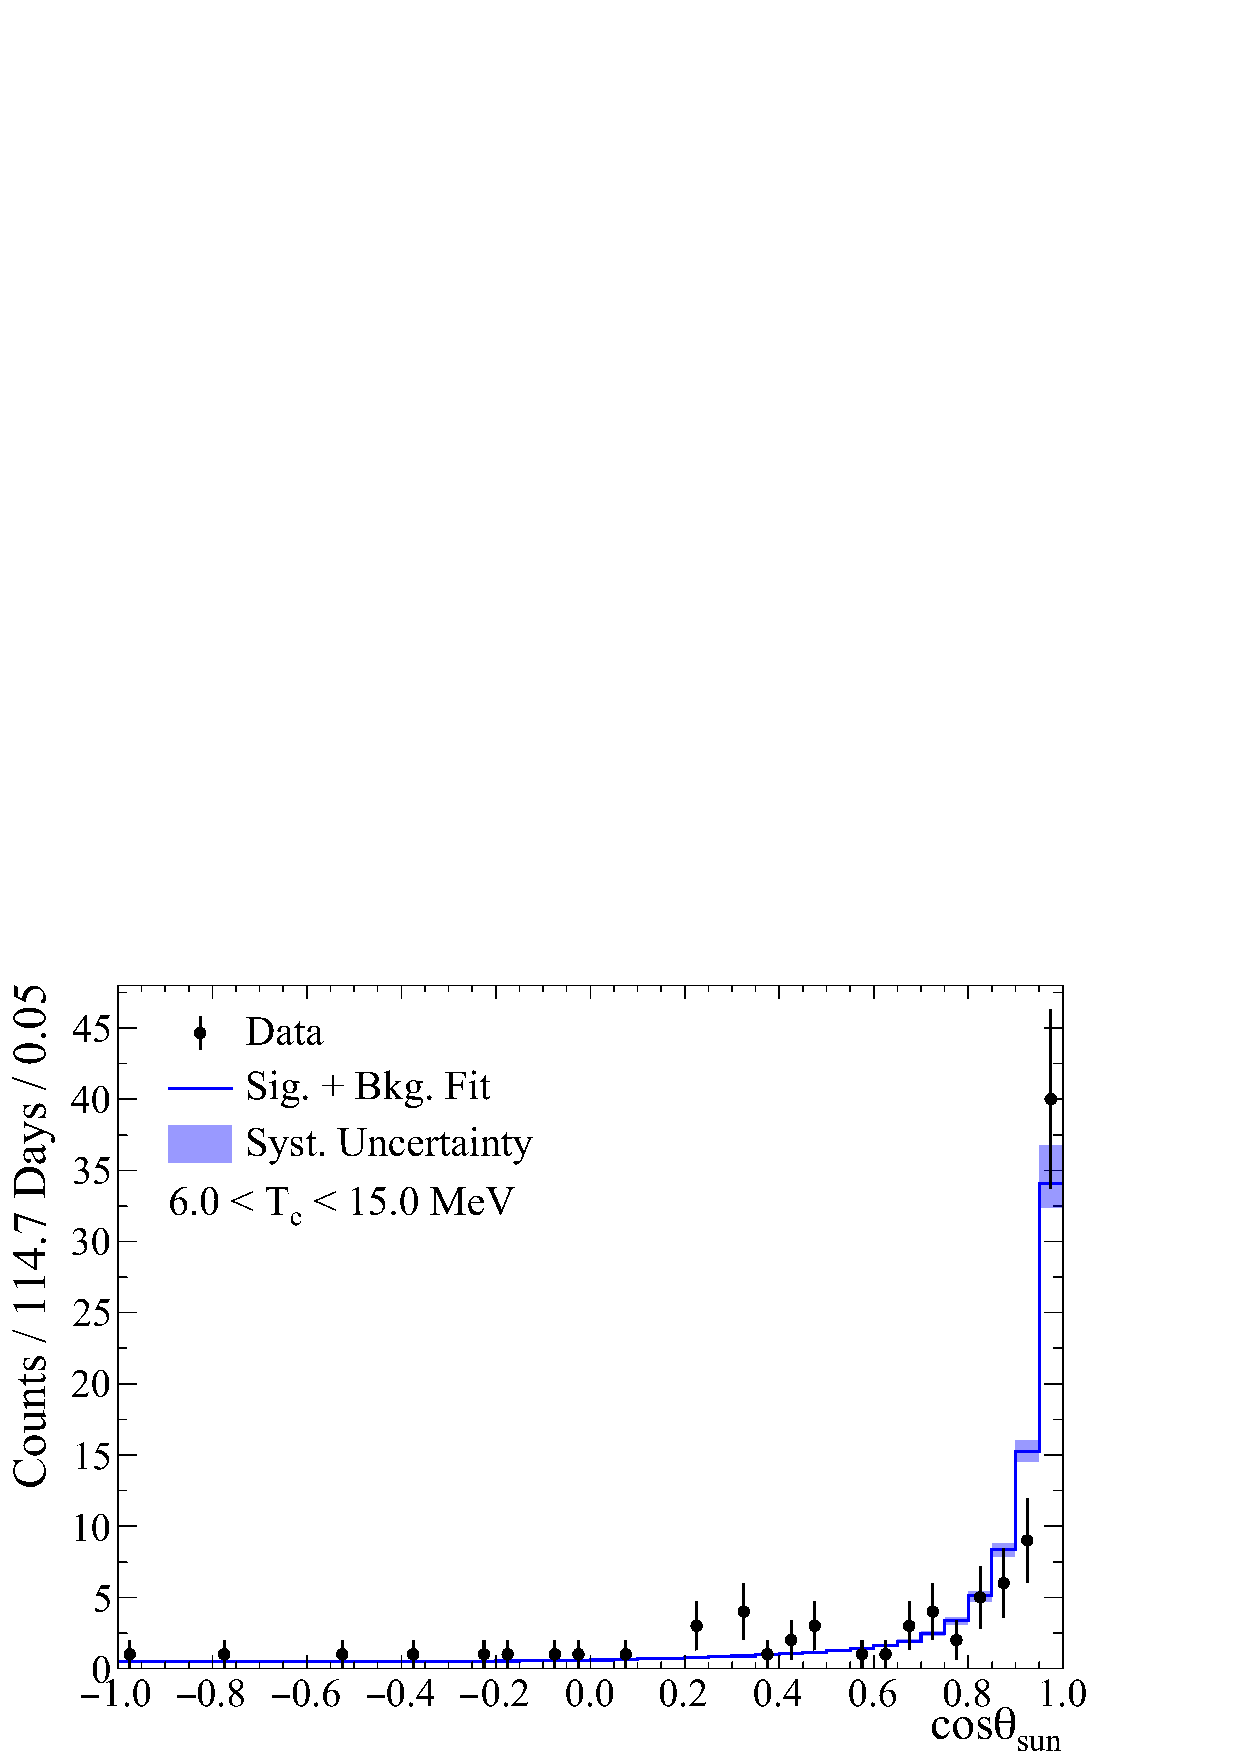
\includegraphics[width=0.5\textwidth]{figures/cos_theta_6mev.pdf}%
\caption{Distribution of event directions with respect to solar direction for
    events with energy in \numrange[range-phrase=--]{6.0}{15.0}\,MeV.}
\label{fig:cos_theta_six}
\end{figure}

The upper five energy bins, \numrange[range-phrase=--]{6.0}{15.0}\,MeV, were an
extremely low background region for this analysis.\
There was very little background contamination from
cosmogenically produced isotopes due primarily to depth of the detector.\
The comparatively high rate of backgrounds in the \numrange[range-phrase=--]{5.0}{6.0}\,MeV bin
comes primarily from decays of radioactive isotopes, such as radon, within the detector.\
Figure~\ref{fig:cos_theta_six} shows the distribution in $\cos\theta_\text{{sun}}$ of events at
energies above 6~MeV, illustrating the low background rate.\
In that energy region the best fit background rate was \LowBackgroundRate, much
lower than the measured solar rate in that energy range, \HighEnergySolarRate.\
For the region above 6~MeV, this is the lowest
background elastic scattering measurement of solar neutrinos in a water
Cherenkov detector.\

